\documentclass[12pt]{amsart}
\usepackage[dvipsnames]{xcolor}
\usepackage{fullpage,graphicx,amsmath,amsfonts, amssymb,enumitem, hyperref, nicefrac,esint}
\usepackage[longnamesfirst]{natbib}
\title{Random walk on sphere packings and Delaunay triangulations in arbitrary dimension}
\author{Ahmed Bou-Rabee}
\address{
	Ahmed Bou-Rabee \\
	Department of Mathematics \\
	University of Pennsylvania \\
	David Rittenhouse Laboratory \\
	209 South 33rd Street \\
	Philadelphia, PA 19104 \\
	Email: ahmedmb@gmail.com
}

\author{Ewain Gwynne}
\address{
	Ewain Gwynne \\
	Department of Mathematics \\
	University of Chicago \\
	Eckhart Hall \\
	5734 S University Ave \\
	Chicago IL, 60637 \\
	Email: ewain@uchicago.edu
}
\subjclass[2020]{Primary 60G50; Secondary 60K37, 65M08}



%% fixes hyperlink colors
\hypersetup{
	colorlinks=true,
	linkcolor=NavyBlue,
	urlcolor = RoyalBlue,
	citecolor = PineGreen
}




\newcommand{\ewain}[1]{{\color{blue}{#1}}}
\newcommand{\ahmed}[1]{{\color{purple}{#1}}}
\newcommand{\td}[1]{\textbf{\color{red}{[#1]}}}

%Equation numbers by section
\numberwithin{equation}{section}

\DeclareMathOperator{\ones}{\mathbf 1}
\DeclareMathOperator{\sgn}{\mathop{\bf sgn}}
\DeclareMathOperator{\R}{\mathbb{R}}
\DeclareMathOperator{\C}{\mathbb{C}}
\DeclareMathOperator{\Z}{\mathbb{Z}}
\DeclareMathOperator{\N}{\mathbb{N}}
\DeclareMathOperator{\Q}{\mathbb{Q}}
\DeclareMathOperator{\A}{\mathbb{A}}
\DeclareMathOperator{\symm}{{\mbox{\bf S}}}
\DeclareMathOperator{\diam}{{\mathop{diam}}}
\DeclareMathOperator{\SLE}{{\mbox{SLE}}}

\DeclareMathOperator{\nullspace}{{\mathcal N}}
\DeclareMathOperator{\range}{{\mathcal R}}
\DeclareMathOperator{\Rank}{\mathop{\bf Rank}}
\DeclareMathOperator{\Tr}{\mathop{\bf Tr}}
\DeclareMathOperator{\diag}{\mathop{\bf diag}}
\DeclareMathOperator{\card}{\mathop{\bf card}}
\DeclareMathOperator{\rank}{\mathop{\bf rank}}
\DeclareMathOperator{\conv}{\mathop{\bf conv}}
\DeclareMathOperator{\prox}{\mathbf{prox}}
\DeclareMathOperator{\per}{\mbox{per}}
\DeclareMathOperator{\prev}{\mbox{prev}}



\DeclareMathOperator{\Var}{\mathop{\bf Var{}}}
\DeclareMathOperator{\Cov}{\mathop{\bf Cov{}}}
\DeclareMathOperator{\Prob}{\mathop{\bf Prob}}
\DeclareMathOperator{\Co}{{\mathop {\bf Co}}} % convex hull
\DeclareMathOperator{\dist}{\mathop{\bf dist{}}}
\DeclareMathOperator{\argmin}{\mathop{\rm argmin}}
\DeclareMathOperator{\argmax}{\mathop{\rm argmax}}
\DeclareMathOperator{\epi}{\mathop{\bf epi}} % epigraph
\DeclareMathOperator{\Vol}{\mathop{\bf vol}}
\DeclareMathOperator{\dom}{\mathop{\bf dom}} % domain
\DeclareMathOperator{\intr}{\mathop{\bf int}}
\DeclareMathOperator{\sign}{\mathop{\bf sign}}

\newcommand{\cf}{{\it cf.}}
\newcommand{\eg}{{\it e.g.}}
\newcommand{\ie}{{\it i.e.}}
\newcommand{\etc}{{\it etc.}}
\newcommand{\etal}{\textit{et al}. }
\DeclareMathOperator{\len}{\mathop{len}}
%%additional commands



%%theorems
\newtheorem{theorem}{Theorem}[section]
\newtheorem{prop}[theorem]{Proposition}
\newtheorem{fact}[theorem]{Fact}
\newtheorem{cor}[theorem]{Corollary}
\newtheorem{lemma}[theorem]{Lemma}
\newtheorem{claim}{Claim}
\newtheorem{remark}[theorem]{Remark}
\newtheorem{definition}[theorem]{Definition}
\newtheorem{problem}[theorem]{Problem}
\newtheorem{conj}[theorem]{Conjecture}

\newtheorem{theoremA}{Theorem}[section]
\renewcommand{\thetheoremA}{\Alph{theoremA}}


\newtheorem{assumptionD}{Assumption}
\renewcommand{\theassumptionD}{\Alph{assumptionD}}
\setcounter{assumptionD}{3}

%% interior and closure
\newcommand{\cl}{\mathbf{cl}}
\DeclareMathOperator{\inte}{\mathbf{int}}

%% redefine P to refer to probability
\renewcommand*{\P}{\mathbb P}
% \DeclareMathOperator{\E}{\mathop{\mathbb E{}}}


\renewcommand*{\S}{\mathbb S}
\DeclareMathOperator*{\osc}{osc}


%to stop the bib warning
\renewcommand{\Bbb}{\mathbb}

%divergence
\renewcommand{\div}{\mathop{\bf div}}

\newcommand{\indc}{{\boldsymbol{1}}}
\newcommand*{\Zd}{\ensuremath{\mathbb{Z}^d}}
\newcommand*{\Rd}{\ensuremath{\mathbb{R}^d}}
\newcommand*{\supp}{\ensuremath{\mathrm{supp\,}}}
\newcommand{\cu}{\square}
\newcommand{\size}{\mathrm{size}}
\newcommand{\G}{\mathcal{G}}

\newcommand{\V}{\mathcal{V}}
\newcommand{\E}{\mathcal{E}}
\newcommand{\eps}{\varepsilon}
\newcommand{\ep}{\varepsilon}
\newcommand{\CLap}{\boldsymbol{\Delta}}
\newcommand{\Cnabla}{\boldsymbol{\nabla}}
\newcommand{\proj}{\boldsymbol{\mathrm{proj}}}
\newcommand{\projone}{\boldsymbol{\mathrm{proj}^{(1)}}}
\newcommand{\projtwo}{\boldsymbol{\mathrm{proj}^{(2)}}}
\newcommand{\projj}{\boldsymbol{\mathrm{proj}^{(j)}}}

\newcommand{\aDelta}{\hyperref[eq:geometric-laplacian]{{\Delta^{\mathcal{G}}_{\cond}}}}
\newcommand{\cond}{\hyperref[eq:geometric-laplacian]{\mathbf{a}}}
\newcommand{\anabla}{\hyperref[eq:anabla]{{\nabla^{\mathcal{G}}_{\cond}}}}
\newcommand{\D}{\hyperref[eq:dir.energy]{\mathcal{D}}}

\newcommand{\GCU}{\hyperref[eq:graph-closure]{\widehat{U}}}
\newcommand{\Qe}{\hyperref[eq:qeset]{Q_e}}
\newcommand{\Lyone}{\hyperref[eq:line-project]{L_y^{(1)}}}
\newcommand{\Lyj}{\hyperref[eq:line-project]{L_y^{(j)}}}

\DeclareMathOperator{\vol}{\mathbf{vol}}
\DeclareMathOperator{\dvol}{\mathbf{d vol}}

\newcommand{\B}{\mathbb{B}}

\DeclareMathOperator{\hm}{\mathop{hm}}
\DeclareMathOperator{\hmn}{\mathop{hm^{n}}}


\DeclareMathOperator{\dPr}{\mathop{d^{Pr}}}


\newcommand{\GVor}{\mathcal{G}^{\mathrm{Vor}}}
\newcommand{\VVor}{\mathcal{V}^{\mathrm{Vor}}}
\newcommand{\EVor}{\mathcal{E}^{\mathrm{Vor}}}


\newcommand{\red}[1]{\textcolor{red}{#1}}
\newcommand{\blue}[1]{\textcolor{blue}{#1}}


\begin{document}

\begin{abstract}
We prove that random walks on a family of tilings of~$d$-dimensional Euclidean space, with a canonical choice of conductances, converge to Brownian motion modulo time parameterization. 
This class of tilings includes Delaunay triangulations (the dual of Voronoi tesselations)
and sphere packings. 
Our regularity assumptions are deterministic and mild. For example, our results apply to Delaunay triangulations with vertices sampled from a $d$-dimensional Gaussian multiplicative chaos measure. 
As part of our proof, we establish the uniform convergence of certain finite volume schemes for the Laplace equation, with quantitative bounds on the rate of convergence. In the special case of two dimensions, we give a new, short proof of the main result of~\cite{gurel2020dirichlet}.%Gurel-Gurevich--Jerison--Nachmias (2020).
\end{abstract}
\maketitle 

\vspace{-0.6in}


\tableofcontents

\section{Introduction}
\label{sec:intro}

\begin{figure}
	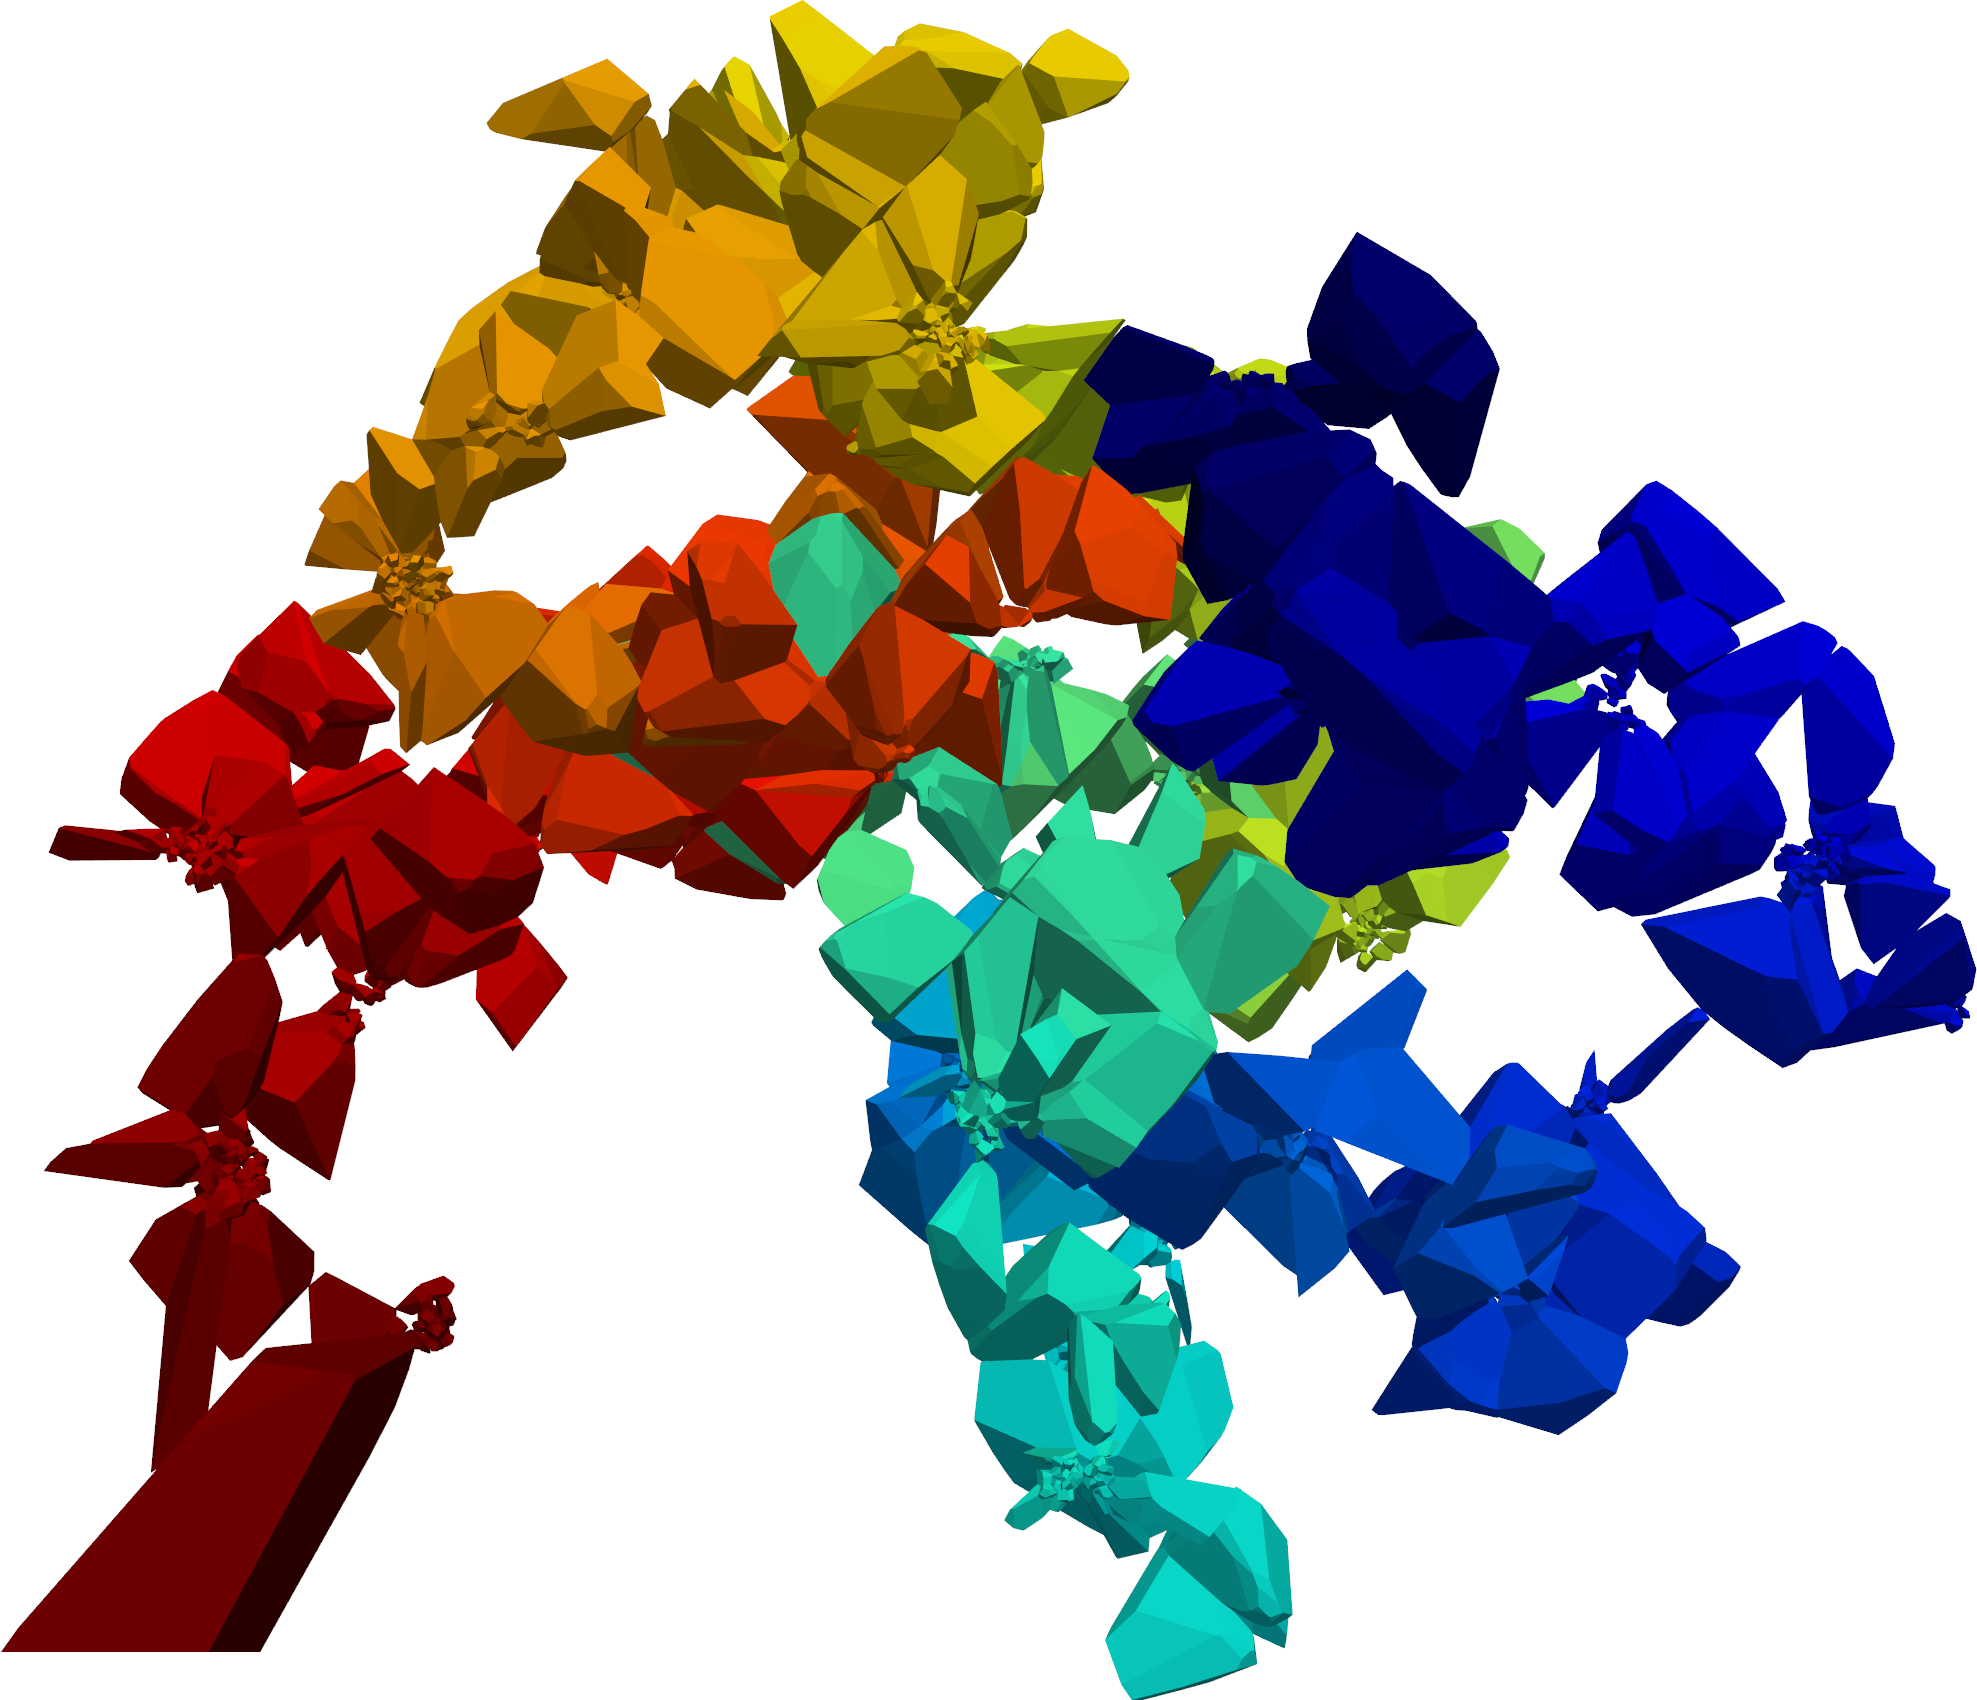
\includegraphics[width=0.79\textwidth]{Figures/x2.png}
	\caption{The trace of random walk on the Voronoi tessalation of $2^{19}$ points sampled from a Gaussian multiplicative chaos measure on a cube with parameter~$\gamma =1$. The random walk is stopped upon exiting the cube and the cells of the tessalation are colored according to the order in which they are visited.}
\end{figure}

In this paper, we consider a class of graphs embedded in $\Rd$, called \emph{orthogonal tilings}, which come equipped with a canonical choice of conductances on their edges (defined in Section~\ref{subsec:main-results}). This class includes tangency graphs of sphere packings as well as $d$-dimensional Delaunay triangulations (the dual graphs of Voronoi tesselations). We show that under nearly minimal regularity assumptions, random walks on these graphs converge to Brownian motion modulo time change, equivalently, discrete harmonic functions converge to their continuum counterparts (Theorems~\ref{theorem:convergence-of-rw-trace} and~\ref{theorem:convergence-of-the-dirichlet-problem}). Several motivations drive this work, and these are discussed in detail in Sections~\ref{subsec:prior} and~\ref{subsec:universality}; to summarize:
\begin{itemize}
\item Orthogonal tilings in~$d=2$ have been studied in part to establish universality of statistical mechanics models, see, for example, the ICM survey,~\cite{smirnovicm}. Our work may be viewed as the first step in this program in~$d \geq 3$. 
\item We obtain a higher-dimensional analog of the results of~\cite{gurel2020dirichlet}, which gives the convergence of discrete harmonic functions on planar orthodiagonal lattices to their continuum counterparts  (see also~\cite{MR1692623},~\cite{chelkaksmirnov}, \cite{skopenkov2013boundary}, and~\cite{werness2015discrete} for earlier results). In the special case when $d=2$, we also obtain a short new proof of the main result of~\cite{gurel2020dirichlet}. 
\item Theorem~\ref{theorem:convergence-of-the-dirichlet-problem} can be viewed as a uniform convergence statement for a class of finite volume approximation schemes for the Dirichlet problem. Such approximation schemes are widely used in numerical analysis, see, for example the textbook~\cite{eymard2000finite}. For the class of approximation schemes considered in this paper, convergence was previously only known in $L^2$, which is not sufficient to get convergence 
of the associated random walk. 
\item Theorems~\ref{theorem:convergence-of-rw-trace} and~\ref{theorem:convergence-of-the-dirichlet-problem} apply to highly inhomogeneous tilings, including certain discretizations of higher-dimensional analogs of Liouville quantum gravity (LQG). The statement that random walk on such discretizations converges to Brownian motion modulo time change can be viewed as a higher-dimensional analog of scaling limit results for random walk on discretizations of LQG in two dimensions~\cite{GMS-Tutte, GMSInvariance}, although the setup and proofs in the present paper are quite different.  
\item Our results provide some evidence that sphere packings and Delaunay triangulations are discrete analogs of conformally flat Riemannian metrics, which suggests that such graphs could possibly play a role analogous to planar maps in higher-dimensional random conformal geometry.  
\end{itemize}



\subsection{Main results}
\label{subsec:main-results}

Let~$\mathcal{D}$ be a subset of~$\Rd$, cover~$\mathcal{D}$ by closed, convex polytopes~$\{P_v\}$ with disjoint interiors, and associate each polytope~$P_v$ with a vertex~$v$ in its interior.  Denote the set of such vertices by~$\V$ and declare that $v,w \in \V$ 
% CORRECTION 1: Make the codimension-one contact convention explicit.
are joined by an edge if $P_v \cap P_w$ has dimension $d-1$ (the contact need not be a full facet of both cells). Assume that each compact subset of~$\mathcal{D}$ intersects finitely many polytopes. We call the resulting graph $\G = (\V,\E)$ a \emph{tiling graph} of~$\mathcal{D}$.  An~\emph{orthogonal} tiling graph satisfies the additional property that for each edge~$(w,v) \in \E$ the vector~$(w-v)$ is orthogonal to the hyperplane containing~$P_w \cap P_v$. 
As we observe in Section~\ref{subsec:natural-examples} below, examples of orthogonal tilings include Voronoi tessellations and tangency graphs of sphere packings.




In this paper we investigate the large scale behavior of random walk on orthogonal tilings. The random walk~$\{X_t\}_{t \geq 0}$ we consider is discrete time and time homogeneous with transition probabilities~$p$ determined by the geometry of the graph: for an edge $(w,v) \in \E$, we set 
\begin{equation} \label{eq:conductance} 
p(w,v) := \frac{\cond(w,v)}{\cond(w)},   \,  \, \,    \text{where}  \,  \, \,   
\cond(w,v) :=  \frac{\vol_{d-1}(P_w \cap P_v)}{\|w - v\| } \,  \, \,  \, \text{and} \,  \, \,  \, \cond(w) := \sum_{(w,v) \in \E} \cond(w, v) .
\end{equation}
Here, $\vol_{d-1}$ denotes $d-1$-dimensional Lebesgue measure. See Figure~\ref{fig:polytope-neighbors}.
\begin{figure}
	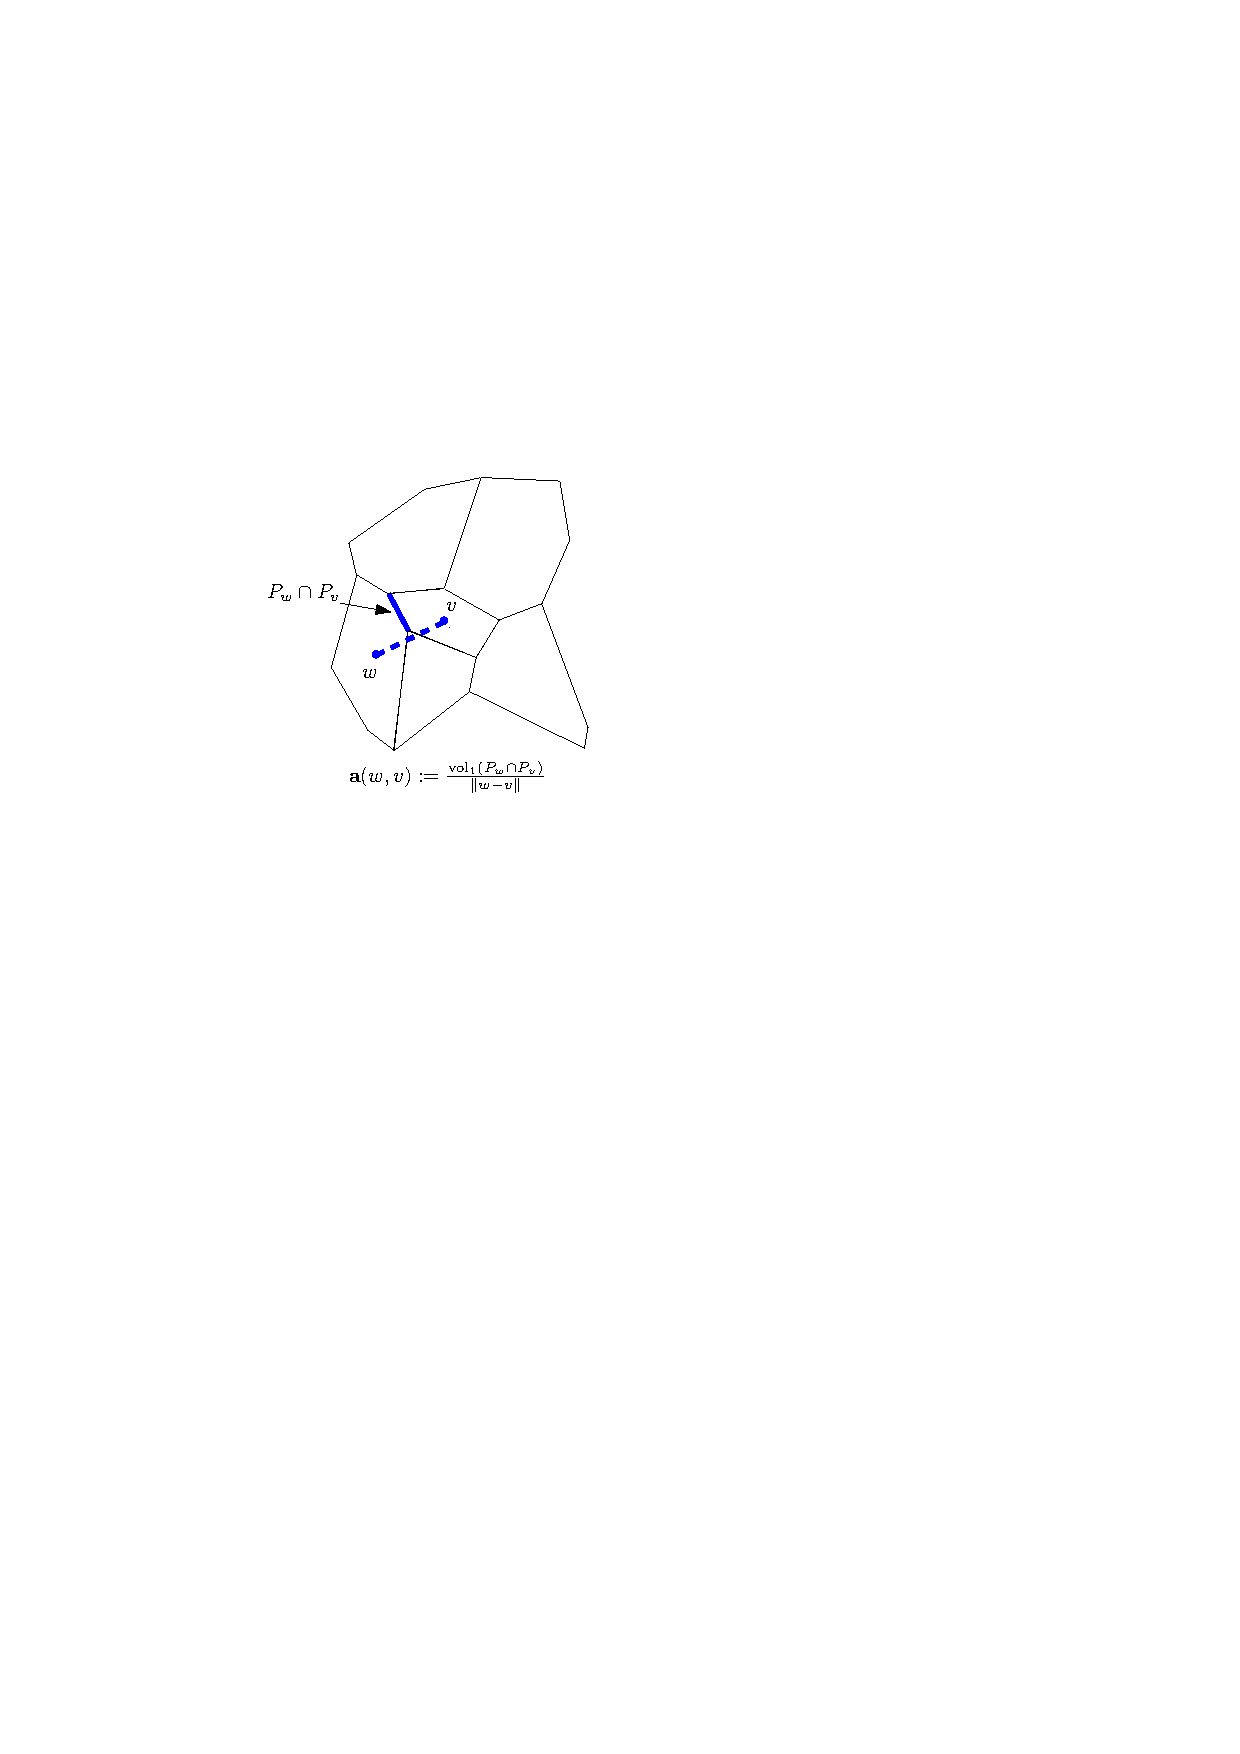
\includegraphics[width=0.4\textwidth]{Figures/polytope-neighbors.pdf}
	\caption{A polytope~$P_v$ and some of its neighbors in an orthogonal tiling. The edge between~$v$ and~$w$ (blue dots) is a blue dotted line and the facet~$P_w \cap P_v$ is a thick blue line. The conductance~$\cond(w,v)$ is the length of the facet divided by the Euclidean distance~$\|w-v\|$.} \label{fig:polytope-neighbors}
\end{figure}

 These probabilities ``tilt" the random walk so that 
% CORRECTION 4: The martingale assertion applies up to the first incomplete cell.
its Euclidean position, stopped at the first vertex with an incomplete cell, is a discrete-time martingale, see Lemma~\ref{lemma:linear-lie-in-kernel} and~\cite[Proposition 6.4]{MR4425348}. In fact, simple random walks on orthogonal tilings do not necessarily converge to Brownian motion modulo time change, even under very strong regularity assumptions --- see Theorem~\ref{theorem:counter-example} below. 
 

The main result of this paper gives the convergence of $\{X_t\}_{t\geq 0}$ to Brownian motion modulo time parametrization. 
We recall the definition of the topology on curves modulo time parametrization from~\cite[Section 2]{AB1999}.
Let~$T_1,T_2 > 0$ and let~$\phi_1: [0,T_1] \to \Rd$ and~$\phi_2:[0,T_2] \to \Rd$ be two continuous 
curves. We define 
\begin{equation}
	\label{eq:cmp-topology}
	d(\phi_1, \phi_2) := \inf_{\psi} \sup_{t \in [0,T_1]} | \phi_1(t) - \phi_2(\psi(t))| \, , 
\end{equation}
where the infimum is taken over all increasing homeomorphisms~$\psi:[0,T_1] \to [0,T_2]$. 




\begin{theoremA}[Convergence of random walk] \label{theorem:convergence-of-rw-trace}
	Let~$U \subset \Rd$ be a bounded, Lipschitz \footnote{We need to assume the domain is Lipschitz because we need that Brownian motion started near the boundary exits the domain close to its starting point. Without this condition, the random walk could exit the domain much earlier than the Brownian motion.} 
% CORRECTION 1: The main convergence results require an ambient collar.
domain such that~$\overline{U}\subset \intr\mathcal{D}$ and let~$\{\G_n\} = \{(\V_n, \E_n)\}$ 	be a sequence of orthogonal tilings of~$\mathcal{D}$. For~$z \in \mathcal{D}$, let~$z^{n}$ be the nearest
	vertex in~$\G_n$ to~$z$ with ties broken in lexicographical ordering. Assume that  
	\begin{equation}
		\label{eq:smallness}
	 \lim_{n \to \infty} \left( \eps_n + \sup_{z \in \mathcal{D}} \|z^{n} - z\| \right) = 0  , \quad \text{where} \quad
	 \eps_n := \sup_{v \in \V_n} \diam(P_v)  
	\end{equation}
	and at least one of the following three conditions is satisfied:
	\begin{enumerate}[label = (\Roman*)]
		\item planarity,~$d = 2$; or \label{item:planarity}
		\item the volume of the smallest tile in~$\G_n$ is at least~$exp( -o(\eps_n^{-1}))$; or \label{item:vol}
		\item there exists $\alpha> 0$ such that the diameter of each tile~$P_v$ in~$\G_n$ is at most \\ $O(\max_{(v,w) \in \E_n} \|w-v\|^{\alpha} \vol_{d-1}(P_w \cap P_v)^{\alpha})$, where the max is over all edges incident to $v$. 
		  \label{item:diam}
	\end{enumerate}
	Then, for each~$z \in U$, as~$n \to \infty$, the linearly interpolated random walk~$\{X_t\}$
	started at~$z^{n}$ and stopped upon exiting~$U$ 
	converges in law to standard Brownian motion started at~$z$ and stopped upon exiting~$U$ with respect to the metric on curves viewed modulo time parametrization~\eqref{eq:cmp-topology}. Moreover, the convergence is uniform over all choices of $z$.
\end{theoremA}



The hypothesis~\eqref{eq:smallness} is close to necessary for the conclusion of Theorem~\ref{theorem:convergence-of-rw-trace} to hold. 
The hypotheses~\ref{item:vol} and~\ref{item:diam} are quite mild and are true for essentially any models one might be interested in, even discretizations of rough, fractal geometries (see Proposition~\ref{prop:min-max-edge-length}). However, we do not know whether it is necessary to have one of these two hypotheses for $d\geq 3$ (see Problem~\ref{problem:hypotheses}).

Hypothesis~\ref{item:vol} can be replaced by a slightly weaker hypothesis concerning the diameters of the connected components of the set of small tiles of $\G_n$, see Theorem~\ref{theorem:generaldim}. This weakened hypothesis is similar to~\cite[Assumption 1.2]{CLM}. We emphasize that in Hypothesis~\ref{item:diam}, we allow any $\alpha > 0$. For $\alpha \not=1/d$, the ratio $\|w-v\|^{\alpha} \vol_{d-1}(P_w \cap P_v)^{\alpha} / \mathrm{diam}(P_v)$ is not scale invariant, so the bound we require is much weaker than a uniform control over the geometry of the tiling at all scales. 
 \smallskip

The macroscopic features of a discrete time Markov process are closely tied to the large scale behavior of its generator, see, \eg, \cite[Theorem 19.25]{MR4226142}. 
% CORRECTION 4: Normalize the discrete-time generator correctly.
An operator with the same harmonic functions as the generator of~$X_t$ is
\begin{equation}
	\label{eq:geometric-laplacian}
	\aDelta h(v) = \sum_{(w,v) \in \E}  \cond(w,v)( h(w) - h(v))
	\quad \mbox{where}  \quad 	\cond(w,v) :=  \frac{\vol_{d-1}(P_w \cap P_v)}{\|w - v\| } , \, 
\end{equation}
% CORRECTION 4: Give the positive vertex factor relating the two Laplacians.
as in~\eqref{eq:conductance}. The discrete-time generator itself is $\cond(v)^{-1}\aDelta$ at $v$.
Theorem~\ref{theorem:convergence-of-rw-trace} is roughly equivalent to the statement that~$\aDelta$-harmonic functions are approximated uniformly, at large scales, by continuum harmonic functions. 

In what follows, we write~$\V_n[U]$ and~$\partial \V_n[U]$ for the set of vertices of $\G_n$ in the interior of~$U$ and those which share an edge with a vertex in the interior, respectively. 
\begin{theoremA}[Convergence of the Dirichlet problem] \label{theorem:convergence-of-the-dirichlet-problem}
% CORRECTION 1: The same ambient collar is needed in both parts of Theorem B.
	Let~$U$ be a bounded domain with $\overline U\subset\intr\mathcal D$ and let~$h_C$ be a function which is harmonic on~$U$. Assume that at least one of the following 
	two conditions hold:  
	\begin{enumerate}[label = (\alph*)]
		\item $h_C$ is harmonic in a neighborhood of~$\overline{U}$; or \label{item:cont-neighborhood}
		\item $h_C$ is continuous on~$\overline{U}$ and $U$ is Lipschitz and~$\overline{U} \subset \mathcal{D}$. \label{item:hypb}
	\end{enumerate}
	 If~$\G_n$ satisfies~\eqref{eq:smallness} and one of \ref{item:planarity}, \ref{item:vol}, or \ref{item:diam} in Theorem~\ref{theorem:convergence-of-rw-trace}, 
	then the discrete harmonic extension~$h^{n}_D$ of~$h_C$ to~$\V_n[U]$, defined by, 
% CORRECTION 2: Sample boundary data at a nearest point of the compact set closure U.
\footnote{In case~\ref{item:hypb}, set the boundary value at $v$ equal to $h_C(\pi_U(v))$, where $\pi_U(v)$ is any nearest point of $\overline U$. Such a point exists by compactness and belongs to $\partial U$ when $v\notin U$. In case~\ref{item:cont-neighborhood}, use $h_C(v)$ for all sufficiently large $n$.}
	\[	
	\left\{	
	\begin{aligned}
		&  \aDelta h^{n}_D = 0 & \mbox{in} & \ \V_n[U] \\
		& h^{n}_D = h_C  & \mbox{on} &  \ \partial \V_n[U]    \, ,
	\end{aligned}
	\right.
	\]
	converges uniformly to~$h_C$,

	\begin{equation}
		\label{eq:convergence-of-d-general}
	\lim_{n \to \infty} \sup_{z \in \V_n[U]} |h^{n}_D(z) - h_C(z)| = 0  \, .
	\end{equation}
\end{theoremA}	
\noindent In fact, we obtain a quantitative bound on the rate of convergence under Assumption~\ref{item:cont-neighborhood} in~\eqref{eq:convergence-of-d-general}, see Theorems~\ref{theorem:2d},~\ref{theorem:generaldim}, and~\ref{theorem:generaldim-decay} below. 



\subsection{Examples}
\label{subsec:natural-examples}

\subsubsection{Sphere packings}

A \emph{sphere packing} is a collection of~$d$-dimensional spheres in~$\R^d$ with disjoint interiors. The spheres are not required to have the same radii. A \emph{sphere-packed graph}, $\G = (\V,\E)$, is the tangency graph of a sphere packing. Each vertex~$v \in \V$ is associated to a sphere~$S_v$ with~$v$ as its centerpoint, and for each edge~$(v, w) \in \E$ there is a unique 
hyperplane~$R_{v,w}$ which is tangent to both~$S_v$ and~$S_w$ at the unique point of $S_v\cap S_w$. A vertex~$v$ is \emph{covered} if 
% CORRECTION 19: A circumscribed polytope is an intersection of halfspaces.
the intersection of the closed halfspaces containing $v$ bounded by the hyperplanes~$\{R_{v,w}\}_{(v,w) \in \E}$ is a bounded $d$-dimensional polytope $P_v$ containing $v$. A sphere-packed graph is~\emph{covering} if every vertex is covered. A sphere packing~\emph{covers} a domain~$U$ 
% CORRECTION 19: Bounded circumscribed cells alone need not form a tiling.
if every vertex is covered and the associated polytopes form a locally finite tiling of a neighbourhood of $U$, with codimension-one contacts precisely the tangency pairs. The tiling requirement is an additional condition; boundedness of the circumscribed polytopes alone does not imply it. 
It is immediate from the definitions that a locally finite sphere packed graph which covers a domain is an orthogonal tiling of that domain. 



\subsubsection{Voronoi tesselations and Delaunay triangulations}

The~\emph{Voronoi tesselation} of a locally finite set of points~$S \subset \Rd$, is the partition of~$\Rd$
into cells~$\{\mathcal{C}_s\}_{s \in S}$ such that every point in the tile~$\mathcal{C}_s$ is closer
to~$s$ than any other point~$s' \in S$, 
\[
\mathcal{C}_s = \{y \in \Rd: \|s - y\| \leq \|s' - y\| \quad \forall s' \in S  \} \, . 
\]
Equivalently, see, \eg ,\cite[Section 1]{mollerLectures}, the cell~$\mathcal{C}_s$ is the intersection, 
over all~$s'\in S$ with~$s' \neq s$ of the closed halfspace 
containing~$s$ and bounded by the bisecting hyperplane of~$s$ and~$s'$, 
\begin{equation}
	\label{eq:half-space-definition-of-cells}
	\mathcal{C}_s = \bigcap_{s' \in S : s' \neq s} \{ y \in \Rd:  (y - \frac{1}{2}(s + s')) \cdot (s-s') \geq 0 \} \, . 
\end{equation}
Consequently, cells are closed~$d$-dimensional convex sets; and for any two neighbors~$s,s'$, the
vector~$(s-s')$ is orthogonal to the~$(d-1)$-dimensional facet~$\mathcal{C}_s \cap \mathcal{C}_{s'}$.
If the cells are finite we denote the orthogonal tiling induced by the Voronoi tesselation of a point set~$S \subset \Rd$ by~
\begin{equation}
	\label{eq:voronoi-tiling-graph}
	\GVor(S) = (\VVor(S), \EVor(S)) \, .
\end{equation}
% CORRECTION 19: A degenerate Voronoi dual need not be a triangulation.
This is the~\emph{Delaunay graph}; in general position it is the graph of the Delaunay triangulation.

Let $U\subset \Rd$ be a bounded domain. Let~$\mu$ be a Radon measure defined in a neighborhood of $\overline U$
which satisfies, for some exponents~$\beta^{\pm} > 0$, for all sufficiently small~$r \in (0,1)$, the bound 
\begin{equation}
	\label{eq:holder-assumption}
	r^{\beta^{+}} \leq \mu(B_r(z)) \leq r^{\beta^{-}} \,  \ 
% CORRECTION 3: The Poisson estimates need mass bounds in a fixed collar.
\quad \forall z \in W ,\qquad W\text{ open},\quad\overline U\subset W , 
\end{equation}
	where~$B_r(s)$ is the Euclidean ball of radius~$r$ centered at~$s \in \Rd$. 
The following proposition implies that Hypothesis~\ref{item:vol} is satisfied  by~$\GVor(\Lambda_m)$,
where~$\Lambda_m$ is a Poisson point process of intensity~$m \mu$, for large~$m$ almost surely.
\begin{prop}
	\label{prop:min-max-edge-length}
	Let~$U$ be a bounded domain.
	With probability one, for all sufficiently large~$m$, the cells of the Voronoi tesselation of~$\Lambda_m$
	which intersect~$U$ satisfy, 
	\begin{equation}
		\label{eq:cells-are-contained-in-balls}
	B_{m^{-8/\beta^-}}(s) \subset \mathcal{C}_s \subset B_{m^{-1/(3\beta^+)}}(s) \qquad \forall s \in \Lambda_m  \mbox{ with~$\mathcal{C}_s \cap U \neq \emptyset$} \, .
	\end{equation}
% CORRECTION 3: Only the cells in a fixed neighbourhood are needed for the Poisson application.
	In particular,the conclusions of Theorem~\ref{theorem:convergence-of-the-dirichlet-problem} and, if~$U$ is Lipschitz, Theorem~\ref{theorem:convergence-of-rw-trace}, hold as $m\to\infty$. Here the tiling consists of the Voronoi cells meeting a fixed bounded neighbourhood $\mathcal D$ of $\overline U$ with $\overline{\mathcal D}\subset W$; the walk is stopped on leaving $U$. No boundedness of all the cells of the global point process is asserted.
\end{prop}



\begin{remark} \label{remark:gmc}
% CORRECTION 3: The GMC application is local inside the field domain.
	Let $\Phi$ be a log-correlated Gaussian field on a domain $W \subset \Rd$, let $U$ be a bounded domain with $\overline U\subset W$, and let $\gamma \in (0,\sqrt{2d})$. Let $\mu = ``e^{\gamma \Phi(x)} \,dx_1\dots dx_d"$ be the associated Gaussian multiplicative chaos (GMC) measure. It follows from standard estimates for GMC that there exists $\beta^\pm = \beta^\pm(d,\gamma)> 0$ such that 
% CORRECTION 3: State the GMC mass estimate on compact subsets of the field domain.
a.s.~\eqref{eq:holder-assumption} holds on any fixed neighbourhood of $\overline U$ whose closure is a compact subset of $W$, for all sufficiently small $r\in (0,1)$ (how small is random). For example, this can be deduced from~\cite[Theorem 3.26]{berestycki2024gaussian} and a union bound argument. Hence, Proposition~\ref{prop:min-max-edge-length} applies to GMC measures on domains in $\Rd$.
	%Expected number of balls with $\mu(B_r(z)) > r^\beta$ is at most $r^{(d+\gamma^2/2) q -\gamma^2 q^2/2 - q \beta - d}$ for any $q \in (0, 2d/\gamma^2)$. There exists a value of $q$ for which the exponent is positive provided $\beta < d  -\sqrt{2d}\gamma  + \gamma^2/2$. 
\end{remark}




\subsubsection{Orthodiagonal maps}
\label{subsection:orthodiagonal}
\begin{figure}
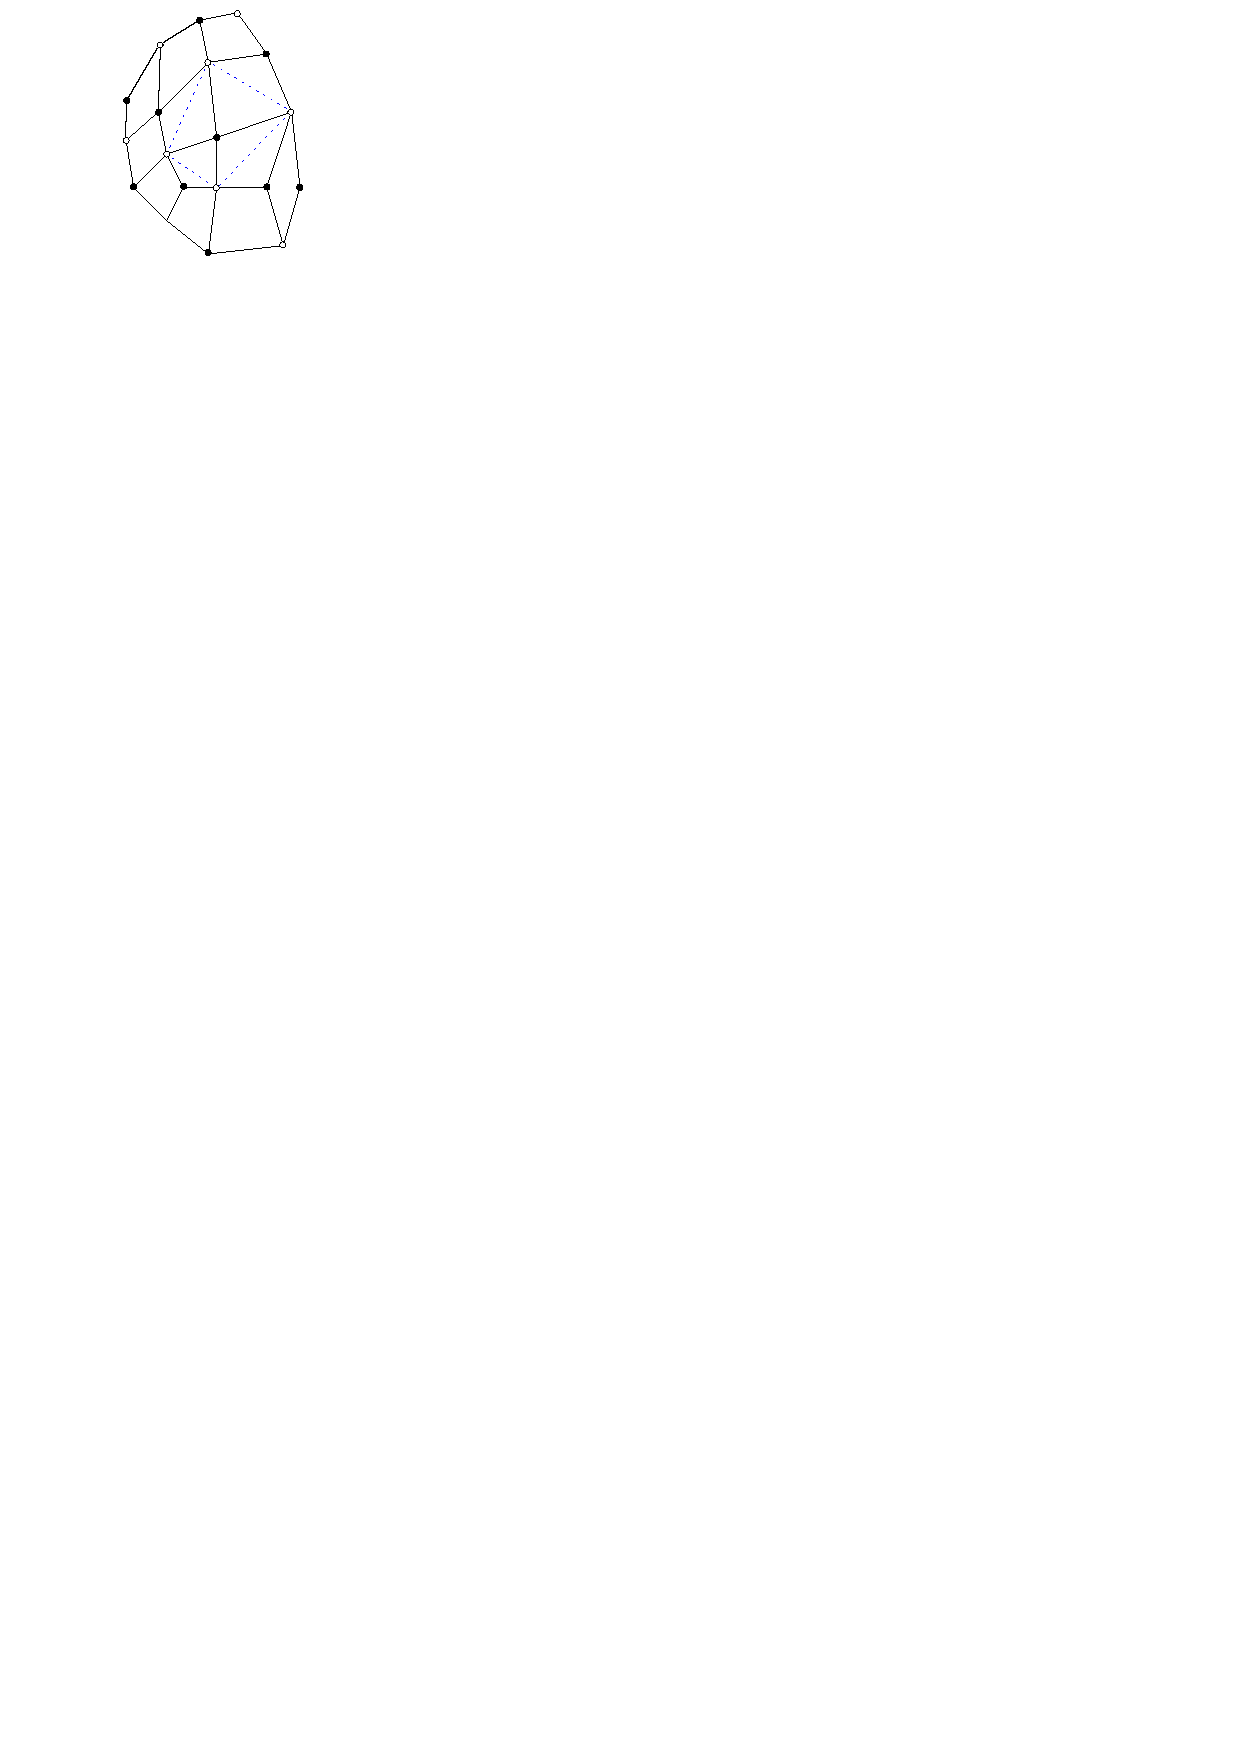
\includegraphics[width=0.3\textwidth]{Figures/orthodiagonal2.pdf}
\caption{An orthodiagonal map. The vertices in~$\V^{\bullet}$ ($\V^{\circ}$) are black (white) and the edges~$\E$ are black lines.
The polytope corresponding to the center vertex is outlined in dotted blue.
 } 
\label{fig:orthogonal-diagonal}
\end{figure}



An \emph{orthodiagonal} map is a finite connected planar graph in which each edge is a straight line segment, each inner face is a quadrilateral with orthogonal diagonals; and the boundary of the outer face is a simple closed curve. An orthodiagonal map 
can be expressed as~$\G = ([\V^{\bullet}, \V^{\circ}], \E)$, where~$\V^{\bullet}, \V^{\circ}$ is a bipartition of the vertices of the graph. 
The vertices~$\V^{\bullet}$ induce a graph~$\G^{\bullet} = (\V^{\bullet}, \E^{\bullet})$ where there is an edge between two vertices~$v_1, v_2 \in \V^{\bullet}$, if they lie on the same inner face of~$\G$. The vertices~$\V^{\circ}$ similarly induce a graph~$\G^{\circ} = (\V^{\circ}, \E^{\circ})$. Isoradial graphs, discussed at the beginning of Section~\ref{subsec:universality} below, can be represented as an orthodiagonal map, see~\cite[Section 2.2]{gurel2020dirichlet}.

The conductance of an edge~$(v_1, v_2)$ corresponding to the inner face of a quadrilateral $(v_1, w_1, v_2, w_2)$ is given by 
\[
\mathbf{a}(v_1, v_2) := \frac{ \|w_1 - w_2\|}{\|v_1 -v_2\|} \, . 
\]
It was shown in~\cite{gurel2020dirichlet} that functions~$f: \V^{\bullet} \to \R$ which are~$\mathbf{a}$-discrete harmonic, that is, which satisfy,
\[
\sum_{(v, w) \in \E^{\bullet}} \mathbf{a}(v, w) (f(v) - f(w)) = 0  \, , 
\]
are close to continuous harmonic functions (in the sense of Theorem~\ref{theorem:convergence-of-the-dirichlet-problem}). 

When every quadrilateral in~$\G$ is convex,~$\G^{\bullet}$ can be represented as an orthogonal tiling. Each vertex~$v \in \V^{\bullet}$
which is not on the outer face of~$\G$ has a polytope~$P_v$ with edges given by the opposite diagonals of the quadrilaterals
containing~$v$ --- that is for each internal face~$(v, w, v', w')$ of~$\G$ with~$v' \in V^{\bullet}$ and~$w,w' \in V^{\circ}$  the edge~$(w, w')$ --- see Figure~\ref{fig:orthogonal-diagonal}. It is straightforward to see for each~$v, v' \in \V^{\bullet}$ that~$\mathbf{a}(v, v')$ coincides
with the conductance defined in~\eqref{eq:geometric-laplacian} and that convexity of each quadrilateral ensures~$v$ is contained in the interior of~$P_v$ and that~$P_v$ is a simple, convex polygon.


% Enumerate the vertex~$v$'s neighbors~$v_1, \ldots, v_n \in \V^{\bullet}$ in counterclockwise order. For~$j = 1, \ldots n$, each neighbor~$v_j$ is a vertex on the quadrilateral~$(v, w_j, v_j, w_{j+1})$ where~$(w_j, w_{j+1}) \in \E^{\circ}$ is fully contained in the quadrilateral 
%(this is where convexity is used) and~$w_{n+1} := w_1$. Since each edge~$(w_j, w_{j+1})$ is contained in the corresponding quadrilateral, the path~$(w_1, w_2, \ldots, w_n, w_1)$ defines a simple polygon. To see that the polygon is convex, identify each vertex with its point in~$\C$
%and observe that~$\arg(\frac{w_{j+1} - w_j}{w_j - w_{j-1}}) \in (0,\pi)$. Indeed, by orthogonality,~$(w_{j+1}-w_j) = i \lambda_j (v_{j}  -v)$
%for some~$\lambda_j > 0$. Since~$\lambda_j$ is real, we have that~$\arg(\frac{w_{j+1} - w_j}{w_j - w_{j-1}}) = \arg(\frac{v_{j+1} - v}{v - v_{j-1}})$. Using that~$v_1, \ldots, v_n$ are in counterclockwise order around~$v$ and each quadrilateral is convex, we have that~$ \arg(\frac{v_{j+1} - v}{v - v_{j-1}}) \in (0,\pi)$. Selecting this polygon to be~$P_v$, it is clear from the above construction~$\cond(v, v_i) = \mathbf{a}(v, v_i)$. 



We describe how to adapt our proof to the case where non-convex quadrilaterals are allowed in Remark~\ref{remark:orthodiagonalmaps} below.




\subsection{Prior work and proof idea}
\label{subsec:prior}

The equation~\eqref{eq:geometric-laplacian} is a~\emph{finite volume scheme} on~$\G_n$ and it is well known that the convergence in Theorem~\ref{theorem:convergence-of-the-dirichlet-problem} holds (with no additional assumptions on~$\G_n$) in~$L^2$, see, \eg, \cite[Theorem 9.3]{eymard2000finite}. Briefly, a finite volume scheme is a numerical method for solving divergence-form elliptic partial differential equations. The domain is partitioned into ``control volumes'' and integrating the equation by parts
on each volume leads to a finite set of constraints. In the case of the Laplacian on orthogonal tilings this gives the operator~$\aDelta$. 

 Our main contribution can be thought of as an~$L^2$ to $L^{\infty}$ estimate for the operator~$\aDelta$ under very weak regularity assumptions on the graph.  As discussed above, these weak assumptions allow the result to apply to highly inhomogeneous random graphs arising from approximations of random fractal geometries. 

$L^2$ to $L^\infty$ estimates are established in previous work when~$\aDelta$ is \emph{uniformly elliptic}, that is, when~$\cond$ is bounded uniformly from above and below, see for example~\cite[Proposition 5.3]{delmotte} for an interior~$L^2$ to $L^{\infty}$ estimate for discrete harmonic functions. The main difficulty in proving Theorem~\ref{theorem:convergence-of-the-dirichlet-problem} is that, in general, the operator~$\aDelta$ is not uniformly elliptic~\emph{at any scale}. 

We prove~\eqref{eq:convergence-of-d-general} by an iteration of an~$L^2$ bound (Proposition~\ref{prop:energy-bound}) and a Poincar\'e type inequality (Lemma~\ref{lemma:ptype-inequality}). The proof, although distinctly different, is reminiscent of the Campanato-type large-scale regularity iteration originating in~\cite{armstrongsmart} and exposited in~\cite[Chapter 4]{AKMBook}. The idea there, which has become a cornerstone of the theory of elliptic homogenization, is that if the solution 
of a heterogeneous equation can be approximated by a harmonic function across a wide range of scales, it should be as regular as harmonic functions.

Here our ``harmonic approximation'', Proposition~\ref{prop:energy-bound}, has an error 
that depends on the continuum harmonic function all the way up to the boundary. Since our graphs are possibly very irregular, there is no immediate way to ``mollify away'' this error. This prevents us from applying the iteration in~\cite{armstrongsmart}. 

Instead, we fix the continuum harmonic function and iterate the discrete approximation. We first show, by the~$L^2$ estimate and a Poincar\'e-type inequality, that the discrete harmonic function,~$h_D$, is pointwise close to the continuum one,~$h_C$, on a dense set of columns (Proposition~\ref{prop:energy-poincare-bound}). The remaining ``bad'' set where~$|h_D - h_C|$ is large has small measure. By Proposition~\ref{prop:energy-poincare-bound} again, the discrete harmonic extension of~$h_C$ to the bad set is close to~$h_C$ on a set of even larger measure. Repeating this, using one of assumptions \ref{item:vol} or \ref{item:diam} in Theorem~\ref{theorem:convergence-of-rw-trace} to close the loop, yields the pointwise bound. 

When~$d=2$, the case which has received the most attention in previous literature, closeness on a dense set of columns and the maximum principle immediately imply the pointwise bound everywhere, yielding a short proof of Theorem~\ref{theorem:convergence-of-the-dirichlet-problem}. This two dimensional result slightly improves~\cite[Theorem 1.1]{gurel2020dirichlet} in that we do not require the domains to be simply connected. 


Earlier work in dimension two, for instance~\cite{MR1692623},~\cite{chelkaksmirnov}, \\ \cite{skopenkov2013boundary}, and~\cite{werness2015discrete}, imposed various assumptions on the graph which ensure that the operator~$\aDelta$ is uniformly elliptic. A similar result for finite volume schemes of a convection diffusion equation in dimensions two and three was also proved (again under assumptions implying uniform ellipticity) in~\cite[Corollary 1]{MR1863279}.



\subsection{Universality and random geometry} 
\label{subsec:universality}
A special case of orthogonal tilings in two dimensions are \emph{isoradial graphs}, graphs which have an embedding into~$\R^2$ so that every face~$F$ of the graph lies on a circle of radius 1 with center in the interior of~$F$.  The term was coined in~\cite{kenyon2002} and a theory of discrete analytic functions on these graphs was developed in~\cite{duffin} and later, independently in~\cite{mercat}. 

Convergence of the Dirichlet problem on isoradial graphs,~\cite{chelkaksmirnov}, was used in a companion paper,~\cite{MR2957303}, to prove
convergence of the critical Ising model, thus establishing~\emph{universality} for the model. 
In an ICM survey~\cite{smirnovicm} asked if these results generalize to other two-dimensional graphs and higher dimensions; in particular, our work addresses~\cite[Questions 1 and 12]{smirnovicm}. This question was also highlighted again in~\cite[Problem 5.9]{skopenkov2013boundary}. 
Several other models have been studied on isoradial graphs including critical dimers, loop-erased random walk, spanning trees, the random-cluster model, and bond percolation; see the survey~\cite{MR3372861} and the papers~\cite{MR3252428, MR3201923,MR3621833, MR3858924}. An interesting next step would be to consider these models for~$d \geq 3$
on orthogonal tilings, see Problem~\ref{problem:lerw} below.

This paper can also be seen as a contribution towards understanding higher-dimensional analogues of discrete conformal geometry and~\emph{Liouville quantum gravity} (LQG). Roughly speaking, LQG is a theory of random geometry in two dimensions which describes the scaling limit of discrete random surfaces, such as uniform triangulations of the sphere, see the surveys~\cite{GwynneSurvey, MR4680280} and the book~\cite{berestycki2024gaussian}. 

There has been recent interest in establishing a corresponding theory in~$d \geq 3$, see, for example,~\cite{schiavo2021conformally, cercle2022, ding2023tightness}. These works study a notion of continuum random geometry in higher dimensions, which is described by a random Riemannian metric tensor of the form $g = e^{\gamma \Phi} g_0$, where $\gamma \in (0,\sqrt{2d})$ is a parameter, $\Phi$ is a log-correlated Gaussian field on a $d$-dimensional manifold (or a minor variant thereof), and $g_0$ is a fixed smooth background metric. If we take $g_0$ to be the flat metric, then (at least at a heuristic level) the random metric tensor $g$ is \emph{conformally flat}, meaning that it is a scalar function times the flat metric. It remains open to determine the correct discrete analog of this continuum theory (analogous to random planar maps in~$d=2$). See, \eg,~\cite[Section 1.2]{ding2023tightness}. The results of this paper contribute to this problem in two respects.


A natural approach to finding a discrete analog of LQG in $d$ dimensions is to search for a class of graphs embedded in $\mathbb R^d$ which satisfy a discrete analog of ``conformal flatness". In~\cite{curienbenjamini} sphere packings were studied partly to understand higher dimensional quantum gravity and it was asked,~\cite[Question 2]{curienbenjamini}, if being representable as the tangency graph of a sphere packing is a discrete analog of being ``conformally flat''. Theorem~\ref{theorem:convergence-of-rw-trace} may be viewed as positive evidence for this, since it implies that the scaling limit of random walk on sphere packings is Brownian motion modulo time change, \ie, in the scaling limit there is no directional bias depending on where the walk is in space.

 Gaussian multiplicative chaos (GMC),~\cite{kahane1985chaos,rhodes2014gaussian,berestycki2024gaussian}, provides the analogue of the LQG area measure in~$d \geq 3$. Voronoi tessellations with centers sampled according to a Poisson point process with respect to GMC (trivially) converge to GMC in the large sample size limit. Thus, Proposition~\ref{prop:min-max-edge-length} and Remark~\ref{remark:gmc} give the convergence to Brownian motion (modulo time change) for random walk on certain embedded random graphs which approximate higher-dimensional analogs of LQG. The first papers to establish this sort of result in two dimensions were~\cite{ GMS-Tutte, GMSInvariance} which prove the convergence of random walk on \emph{mated-CRT maps}, a family of random planar maps known to converge to Liouville quantum gravity. The setting and proof of this result, however, are quite different from the present paper. The proof uses both planarity and the randomness of the environment (whereas here we have a fixed, deterministic environment in arbitrary dimension). Moreover, there are no conductances on the edges of the mated-CRT map, so the random walk is not a martingale (although the proofs show that it is approximately a martingale at large scales). See also Problem~\ref{problem:higherdim-invariance}.







\subsection{Open questions}
We mention some possible directions for future research motivated by our work. 
\begin{problem} \label{problem:lerw}
	What can be said about other statistical mechanics models, \eg, loop-erased random walk, uniform spanning tree, percolation, Ising model, dimers, discrete Gaussian free field, etc., on orthogonal tilings for $d\geq 3$?
\end{problem}


The paper~\cite{GMSInvariance} proves that random walk converges to Brownian motion modulo time change in certain random planar environments which are not stationary with respect to translations, but are instead only ``translation invariant modulo scaling". It is plausible that this result could be extended to dimension $d\geq 3$ if one assumes that the edge conductances scale by $\Lambda^{d-2}$ when one scales space by $\Lambda$, see~\cite[Section 1.5]{GMSInvariance}. It appears that the main obstacle to proving such an extension is transferring from an $L^2$ bound for discrete harmonic functions to an $L^\infty$ bound (this corresponds to Lemma 2.19 in \cite{GMSInvariance}, the proof of which strongly uses planarity).


\begin{problem} \label{problem:higherdim-invariance}
Can the techniques of this paper be used to prove a higher dimensional analogue of \cite{GMSInvariance}?
\end{problem}




A consequence of Theorem~\ref{theorem:convergence-of-rw-trace} is that random walk on Voronoi tessellations with centers sampled from a $d$-dimensional Gaussian multiplicative chaos measure converges to Brownian motion modulo time change. 
The paper~\cite{GB-LBM} proves that random walk on mated-CRT maps converges in law with respect to the uniform topology to \emph{Liouville Brownian motion}, the natural LQG time change of Brownian motion. It would be interesting to establish an analog of this result for the Voronoi tessellations considered in this paper.  

\begin{problem} \label{problem:convergence-to-lqg}
Determine the scaling limit of random walk on Voronoi tessellations with centers sampled from $d$-dimensional GMC viewed as a parametrized path which spends one unit of time in each cell.
\end{problem}


Instead of giving the walk its natural parametrization, we could alternatively seek a time parametrization which makes it converge to standard Brownian motion. To be consistent with Brownian scaling, we need to parametrize so that if we scale space by $\Lambda$, the amount of time spent in each polytope scales like $\Lambda^{2 }$. 

\begin{problem}
	Consider random walk on an orthogonal tiling graph parameterized so that the amount of time
	it spends at each polytope is proportional to the volume of the polytope to the power $2/d$.
	Does this random walk converge to standard Brownian motion? 
\end{problem}




\begin{problem} \label{problem:hypotheses}
For $d\geq 3$, either show that the conclusion Theorem~\ref{theorem:convergence-of-rw-trace} is true without assumption \ref{item:vol} or \ref{item:diam}; or give an explicit counterexample to show that at least one of these assumptions is necessary. 
\end{problem}



\subsection{Paper outline} 
We start in Section~\ref{sec:prelims} with discrete PDE estimates, geometric bounds for orthogonal tilings, and the aforementioned~$L^2$ estimate for~$\aDelta$-harmonic functions. All of the results contained in the section are standard but included for the reader's convenience. In Section~\ref{sec:iteration} we prove Theorem~\ref{theorem:convergence-of-the-dirichlet-problem} under Hypothesis~\ref{item:cont-neighborhood} and at least one of Assumptions~\ref{item:planarity},~\ref{item:vol}, or~\ref{item:diam}. 
Then, in Section~\ref{sec:rw-convergence} we use this to prove Theorem~\ref{theorem:convergence-of-rw-trace} and subsequently deduce Theorem~\ref{theorem:convergence-of-the-dirichlet-problem} under Hypothesis~\ref{item:hypb}. In fact, there we prove a ``black box'' statement asserting, roughly, that whenever one has convergence of the Dirichlet problem, one has convergence of the associated random walk. In Section~\ref{sec:verifying-assumptions} we prove Proposition~\ref{prop:min-max-edge-length}, which verifies that our results apply to graphs derived from Gaussian multiplicative chaos measures. 
Finally, in Section~\ref{sec:counter-example} we give an example of a sphere packing in~$d \geq 3$ for which simple random walk (with unit conductance)
does not converge to Brownian motion modulo time parameterization. 


\subsection*{Conventions and notation}
\begin{itemize}
	\item For a set~$U \subset \Rd$, we denote the~$d$-dimensional Lebesgue measure by $\vol_{d}(U)$
	and we denote its Euclidean diameter by~$\diam(U)$.
	\item For a point~$v \in \Rd$,~$\|v\|$ is the Euclidean norm.
	\item For a point~$v \in \Rd$ and~$r > 0$, we write~$B_r(v)$ for the Euclidean ball of radius~$r$ centered at~$v$. When~$v=0$, we write~$B_r$. 
% CORRECTION 4: Specify edge counting, complete cells, and zero-duration curves once.
	\item Unless explicitly mentioned, we henceforth fix a set~$\mathcal{D}$ and an orthogonal tiling~$\G$ of~$\mathcal{D}$ and denote the set of edges and vertices by~$\E$ and~$\V$ respectively.
        A cell $P_v$ is called complete if
        $\partial P_v=\bigcup_{w\sim v}(P_v\cap P_w)$, with finitely many neighbours.
        In Sections~\ref{sec:prelims}--\ref{sec:iteration}, every active vertex set $A$, including $A=\V[U]$, is assumed to consist of complete cells. Lemmas~\ref{lemma:discrete-divergence-theorem}, \ref{lemma:dual-variational-principle}, and~\ref{lemma:gradient-energy-estimate} do not require completeness; Lemma~\ref{lemma:geometry-bound} is an identity for one edge. Lemma~\ref{lemma:linear-lie-in-kernel} is asserted at complete cells. This permits a cell to meet $\partial\mathcal D$ in a set of lower dimension. Cells contained in $\intr\mathcal D$ are complete: local finiteness and coverage imply that each relative interior point of a facet is covered on its other side, and the finite union of the resulting closed contacts covers the facet.
        Scalar energy and geometric-mass sums count each undirected edge once. The sums in Lemmas~\ref{lemma:discrete-divergence-theorem} and~\ref{lemma:dual-variational-principle} explicitly count both orientations; halving both sides of the latter gives its undirected form.
        Signed sums and divergences on a finite vertex set have finite incident edge sets. Nonnegative energy and mass sums may take extended real values when the index set is infinite. Suprema of nonnegative quantities over empty sets are zero, and $\eps\log(\eps^{-1})$ at $\eps=0$ is its continuous value zero.
        A stopped path of duration zero is the constant curve; curves at distance zero in~\eqref{eq:cmp-topology} are identified. 
	We also denote, for~$e = (w,v) \in \E$, 
	\[
	H_e := P_w \cap P_v \, . 
	\]
	\item In an abuse of notation, we identify vertices~$v \in \V$
	with their location in~$\Rd$ and the edge~$(w,v) \in \E$ with 
	the straight line between~$w$ and~$v$. We also denote the length of the edge~$e = (w,v) \in \E$, by~$\|e\| := \|w - v\|$. 
	
	
	\item 
	The induced subgraph of a domain~$U \subset \Rd$ is~$\G[U]$. It is defined as the set of vertices contained in the interior of~$U$ 
	together with the edges connecting pairs of vertices in that subset --- see Figure~\ref{fig:induced-subgraph}. The edges and vertices of an induced subgraph are~$\E[U]$ and~$\V[U]$ respectively. 
	
	\item The set of edges connecting pairs of vertices in a set~$A$ is denoted by~$\E[A]$. 
	The set of edges in~$\E$ with at least one vertex in~$A$ is~$\E[\overline{A}]$ and~$\partial \E[A] = \E[\overline{A}] \setminus \E[A]$.
	In an abuse of notation, we consider~$\E$ to be a set of both directed and undirected edges. 
	
	
	\item 
	The sets~$\partial U$,~$U^{\circ}$, and~$\overline U$ denote the boundary, interior, and closure of~$U$, a subset of~$\Rd$. 
	\item For a collection of vertices~$A \subset \Rd$, we write~$\partial A$ for the set of vertices in~$\V \setminus A$ which share an edge with a vertex in~$A$
	and~$\overline A = A \cup \partial A$. 
	
	
	\item  
	For a domain~$U \subset \Rd$ we define the set
	\begin{equation}
		\label{eq:graph-closure}
		\GCU :=  \bigcup_{v \in \overline{\V[U]}} P_v  \, , 
	\end{equation}
	as the set of polytopes with vertices in or adjacent to~$U$.
	


	

	
	\item A \emph{vector field}~$\theta$ is a function~$\theta: \E[A] \to \R$ which is antisymmetric:
	~$\theta(w,v) = - \theta(v,w)$ for every~$(w,v) \in \E[A]$. 

	
\end{itemize}

\begin{figure}
	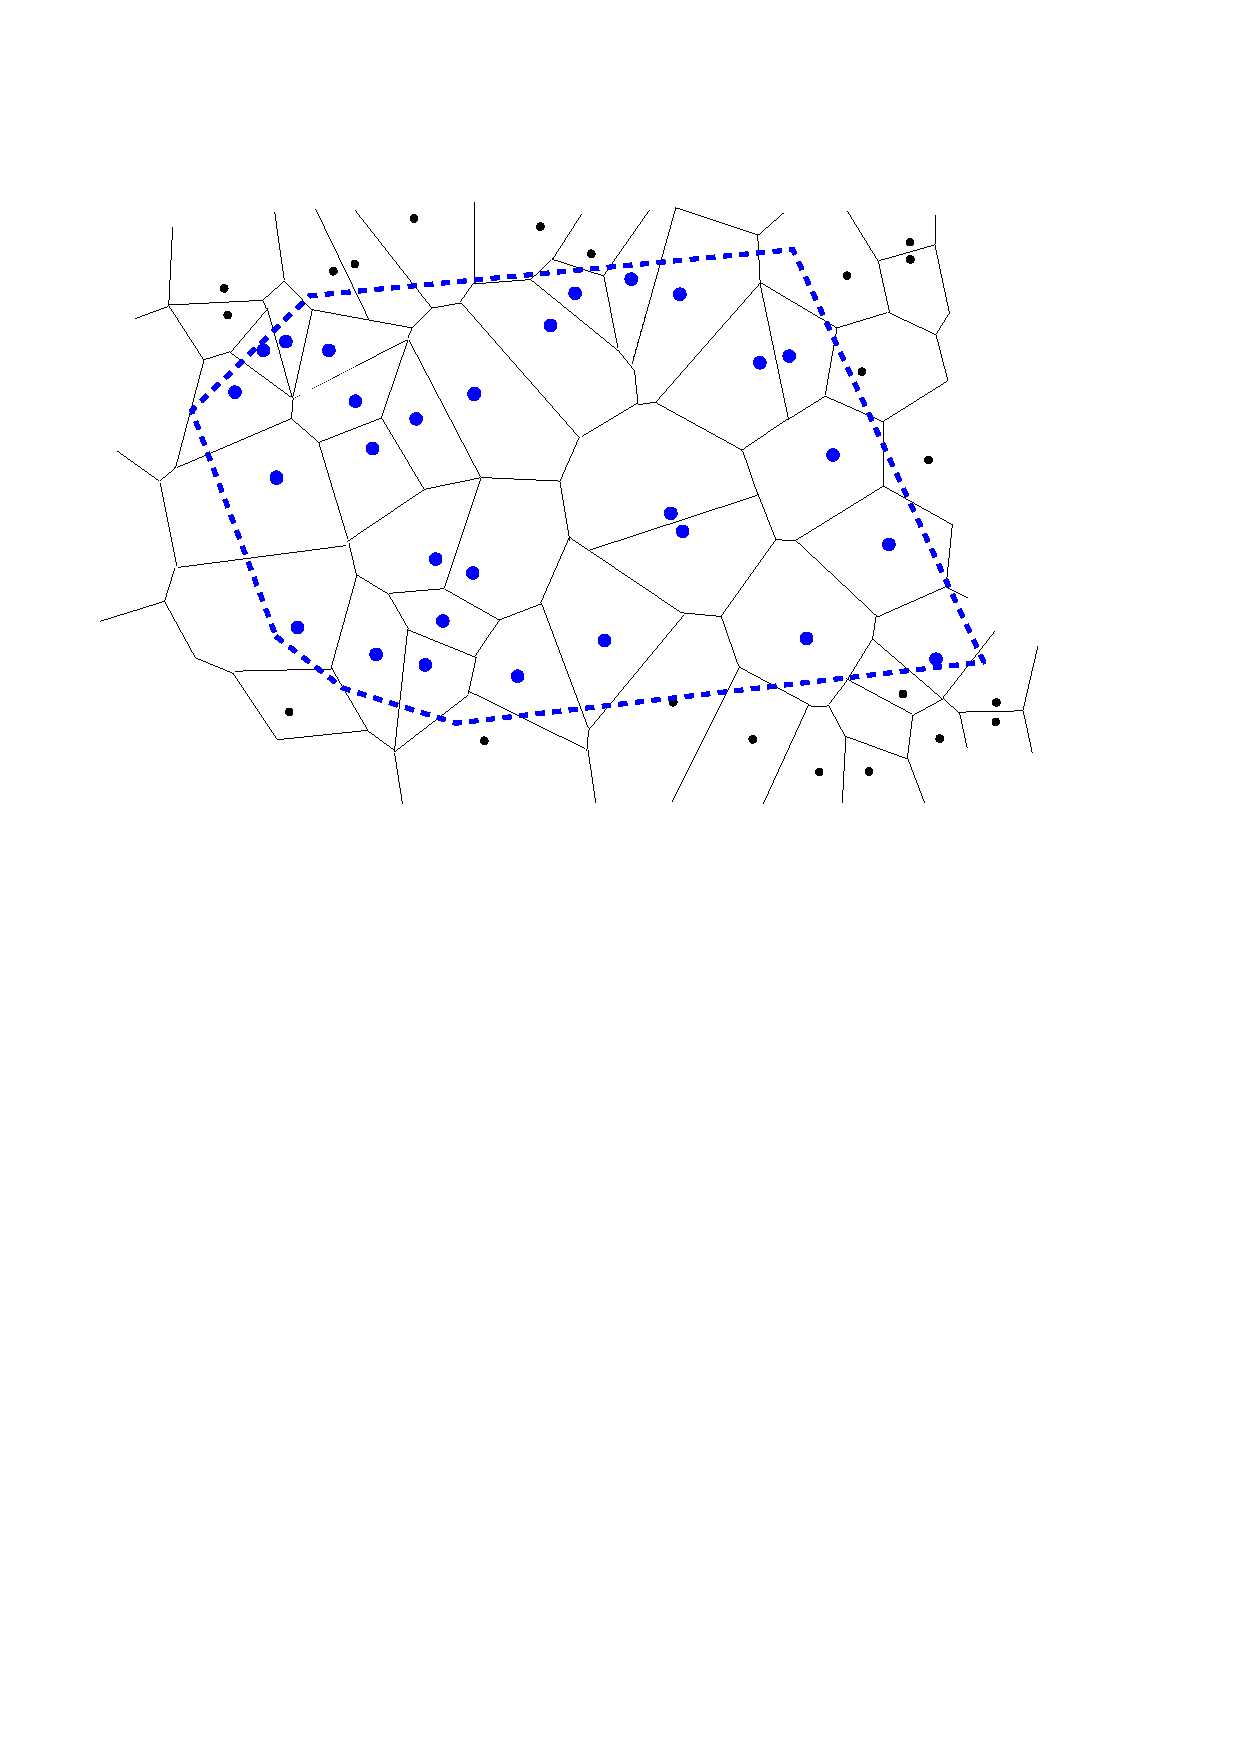
\includegraphics[width=0.5\textwidth]{Figures/induced-graph.pdf}
	\caption{The domain~$U$ is outlined in dashed blue and the vertices of the induced subgraph~$\G[U]$ are blue dots.}
	\label{fig:induced-subgraph}
\end{figure}



\subsection*{Acknowledgments}
Thank you to Gioacchino Antonelli, Scott Armstrong, Bill Cooperman, and Marianna Russkikh for useful discussions and suggestions.
Thank you to Leonardo Bonanno, Jeanne Boursier, Martina Neuman, and the anonymous referee for helpful comments on an earlier
version of this article. 
A.B. was partially supported by NSF grant DMS-2202940. E.G. was partially supported by NSF grant DMS-2245832.





% CORRECTION 18: List the substantive corrections without renumbering the published results.
% CLOSE 9: Update the correction record to state the adopted analytic repairs.
\section*{Corrections to the published version}
The statements retain their published numbering. The following changes specify the geometry, analytic constants, and proof details. For each changed statement we say whether the published version is false, with a counterexample, or open; the other changes concern only proofs or conventions.
\begin{enumerate}
\item The convergence theorems use a neighbourhood of $\overline U$ inside the ambient tiling. The local estimates require that the active cells have no unshared part of a facet. Without these conditions the published statements are false: on a square grid of a rectangle, the walk cannot leave through sides where the cells have facets shared with no other cell, and the discrete solutions there do not converge. The same grid, or two unit squares, shows that Lemmas 2.2 and 3.1, Propositions 2.6 and 3.2 and Theorems 3.3, 3.6 and 3.7 need this facet condition. The position of the walk is a martingale up to the first vertex with an incomplete cell. Codimension-one contacts are understood as in the published flux computations, without requiring full common facets.
\item Boundary data in Theorem B(b) are evaluated at nearest points of $\overline U$. The point specified in the published footnote need not exist, so the published prescription is not always defined. The mass bounds in Proposition 1.1 are imposed in a fixed neighbourhood of $\overline U$, and its tiling is localized there. The published version is false: for the Lebesgue measure restricted to $U$, the extreme cells of the finite Poisson process are unbounded and meet $U$. Remark 1.2 on Gaussian multiplicative chaos is correspondingly local, on compact subsets of the field domain.
\item The finite-degree condition and edge-counting conventions are explicit; without finite degrees the sums in Lemma 2.1 are not defined. The quadratic energy is the square of a seminorm. Lemma 2.5 covers selected cells: its published first inclusion is false, since a small ball inside one square of a grid contains no site. The pyramid map in Lemma 2.4 is corrected to match its Jacobian. The Poincar\'e proof in Lemma 3.1 treats separate components of a line's intersection with the cells.
\item In the sphere-packing example, circumscribed cells are intersections of halfspaces. Their forming a tiling is a separate condition: for example, equal spheres on a nonrectangular rhombic lattice can have bounded circumscribed cells with overlapping interiors. The discrete-time generator is the displayed conductance Laplacian divided by the total conductance at the vertex. A degenerate Voronoi dual is called a Delaunay graph, since its faces need not be simplices.
\item Propositions 2.6 and 3.2 use a constant controlling the cell Hessian and the finite Taylor remainders between adjacent vertices. A Hessian bound along the edge segments is sufficient but is not required. A slit-domain harmonic function gives a counterexample to the published energy bound; a thin reflected Voronoi configuration also refutes the published column bound. The two propositions need the finite Taylor inequality only at one active endpoint of each edge. The three quantitative theorems use the smaller constant $M_U^\circ$ in~\eqref{eq:internal-taylor-constant}, testing only edges with both endpoints active. The cell Hessian alone bounds each normalized boundary flux discrepancy by $M_0\eps^2$. These are revised quantitative statements; no claim is made that the two proposition counterexamples disprove the cell-only versions of the three theorems. Whether the three theorems hold with the published cell Hessian constant alone is open.
\item The displayed planar bound uses a quadratic comparison term and the boundary correction $3M_0\eps^2$, with no local oscillation or between-vertices Lipschitz hypothesis. Optimizing gives an $\eps^{2/3}$ rate, and hence the stated $\eps^{1/2}$ rate, on the explicit small-mesh range $\eps\le1/2$. With a constant uniform over all meshes the published rate is false: for large $\eps$, a product tiling with a large central cell has an error of order $\eps$. This replaces the published linear $L$ term. Whether the published linear bound holds is not settled here. The higher dimensional bounds retain $CMK\eps\log(\eps^{-1})+DL$ and $CM\eps\log(\eps^{-1})$, with $M=M_U^\circ\vee1$. Their iteration uses internal fluxes, includes all boundary contributions, and uses the geometric-decay product $C_0 4^{-\alpha i}$.
\item Proposition 4.2 is localized to balls with closure in the neighbourhood in Assumption D. Without this the published statement is false: a walk that is simple random walk only near a distant point satisfies Assumption D, while the harmonic measure of the unit ball is a point mass. The conventions of Assumption D on test functions and on the choice of solutions are made explicit; the assumption is unchanged. Its proof and the ball coupling in Theorem 4.1 include exit localization and boundary stopping. The proofs transferring these estimates to Theorems A and B specify the fixed collar, the choice $K\geq1$, and boundary-data approximation. Their conclusions are unchanged apart from the ambient collar and the boundary-data convention.
\item The grid tests in Lemma 5.1 include the necessary neighbourhood of $U$. The published part (a) is false: if $U$ contains no grid point its hypothesis is empty, while two sites in $U$ at distance less than $r$ violate its conclusion. In part (b) the published radius $2k$ fails for every $d\ge13$ (a counterexample follows the proof); the lemma is stated with dimension-dependent constants $\delta(d)$ and $R(d)$. For $d\le3$ the proof keeps the published radius $2k$; for $4\le d\le12$ the published radius also suffices with a smaller $\delta$, by a separate rounding argument not needed here. The unchanged polar bound in Lemma 5.2 is proved directly. The Poisson proof uses bounded overlap and also treats cells whose sites lie outside $U$; its exponents are unchanged.
\item Theorem 6.1 retains its statement. In dimensions at least four the small spheres are placed at even coordinates beyond the third, and a harmonic function proves non-convergence. The published count of neighbours at the interface does not hold for all its small spheres, so only the proof changes.
\end{enumerate}

\section{Preliminaries}
\label{sec:prelims}
Here we collect, for completeness, some standard preliminary results that are essentially contained in, \eg, the textbooks~\cite{eymard2000finite, Telcs2006, droniou2018gradient}.


\subsection{Discrete PDE}
We write~$\CLap$ and~$\Cnabla$ for the continuum Laplacian and gradient on~$\Rd$. For a function~$f : \V \to \R$ the vector fields
~$\nabla^{\mathcal{G}} f$ and~$\anabla f$ are defined by,  for a directed edge~$e = (w,v)$, 
\begin{equation}
	\nabla^{\mathcal{G}} f(e) = f(w) - f(v)	
\end{equation}
and
\begin{equation}
	\label{eq:anabla}
\anabla f(e) = \cond(e)(f(w) - f(v)) \, . 
\end{equation}
 The~\emph{divergence} of a vector field~$\theta:\E \to \R$ is the scalar function 
\begin{equation}
	\label{eq:discrete-divergence}
(\div \theta)(v) := \sum_{ (w,v) \in \E } \theta(e) \, , 
\end{equation}
where the sum is over all the directed edges whose endpoint is~$v$. Observe that we can write 
\[
\aDelta h(v) = (\div \anabla h)(v) \, .  
\]


We first recall a version of the discrete divergence theorem. This holds for general graphs
and is well known, but we include a (short) proof. 
\begin{lemma} \label{lemma:discrete-divergence-theorem}
% CORRECTION 5: Finite degrees make the divergence identity well defined on a general graph.
		Let~$A \subset \V$ be a finite set of vertices of finite degree, and let~$f: \overline{A} \to \R$ be a function which is
	zero on~$\partial A$. Then, for any vector field~$\theta: \E[\overline{A}] \to \R$ we have that 
	\begin{equation}
		\label{eq:discrete-divergence-theorem}
	\sum_{v \in A} (\div \theta)(v) f(v) = - \frac{1}{2} \sum_{e \in \E[\overline{A}]} \theta(e) \nabla^{\mathcal{G}} f(e) \, . 
\end{equation}
\end{lemma}
\begin{proof}
	Each neighboring pair of vertices~$\{w,v\}$ appears twice in the sum on the right in~\eqref{eq:discrete-divergence-theorem}, once as~$\theta(w,v) (f(w) - f(v))$
	and again as~$\theta(v,w) (f(v)-f(w)) = \theta(w,v) (f(w)-f(v))$, by antisymmetry of~$\theta$. Consequently, since~$f \equiv 0$ on~$\partial A$, 
	\[
		\sum_{e \in \E[\overline{A}]} \theta(e) \nabla^{\mathcal{G}} f(e) =  \sum_{v \in A} -2 f(v) \sum_{(w,v) \in \E} \theta(w,v)  
		= \sum_{v \in A} -2 f(v) (\div \theta)(v) \, , 
	\]
	which completes the proof.
\end{proof}




The next lemma states that linear functions lie in the kernel of~$\aDelta$. In particular, like the usual Laplacian, the operator~$\aDelta$ has no drift.
% CORRECTION 4: The repaired comparison proofs use affine harmonicity.
This also gives the maximum principle and the quadratic comparisons used below. For a finite set $A$ of complete cells, every graph component of $A$ has an exterior neighbour: otherwise summing
     $\aDelta\|\cdot\|^2(v)=\sum_{w\sim v}\cond(v,w)\|w-v\|^2>0$
     over that component would give zero by cancellation. Hence every finite Dirichlet problem used below has a unique solution, and the associated walk exits almost surely (from each vertex a finite path of positive probability reaches the boundary; take the minimum of these probabilities).
A similar statement in the special case of sphere packings appears as~\cite[Proposition 6.4]{MR4425348}.
\begin{lemma} \label{lemma:linear-lie-in-kernel}
	For every~$p \in \Rd$ and ~$c \in \R$, denoting~$\ell_p(x) = p \cdot x + c$, 
% CORRECTION 4: Affine harmonicity holds at complete cells.
we have that $\aDelta \ell_p(v) = 0$ at every vertex with a complete cell. 
\end{lemma}
\begin{proof}
% CORRECTION 4: Use completeness in the cell flux proof.
	Let~$v \in \V$ have a complete cell and observe that by definition, 
	\begin{align*}
		\aDelta \ell_p(v) = \sum_{(w,v) \in \E} \frac{\vol_{d-1}(P_w \cap P_v)}{\|w - v\|} (\ell_p(w) - \ell_p(v))
		= 
				\sum_{(w,v) \in \E} \vol_{d-1}(P_w \cap P_v) \left( p \cdot \frac{(w-v)}{\|w - v\|} \right)\, . 
	\end{align*}
	By the (continuum) divergence theorem we have
	\[
	0 = \int_{P_v} \CLap \ell_p  = \int_{\partial P_v} \Cnabla \ell_p \cdot \nu
	= \int_{\partial P_v} p \cdot \nu 
	   \, , 
	\]
	where~$\nu$ denotes the outward pointing normal vector field to~$P_v$. By the definition of an orthogonal tiling, whenever $(w,v) \in \E$ we have $\nu = \frac{w-v}{\|w-v\|}$ on $P_v \cap P_w$. Therefore,
	\[
	\int_{\partial P_v} p \cdot \nu  = 	\sum_{(w,v) \in \E} \vol_{d-1}(P_w \cap P_v) \left( p \cdot \frac{(w-v)}{\|w - v\|} \right)\,.  
	\]
	Combining the previous three displays completes the proof. 
\end{proof}



We next recall the dual variational principle for the discrete Dirichlet problem. A continuum version of this appears in, for example, \cite[Section 8.7, Exercise 13]{evans2022partial}. Also see~\cite[Proposition 4.9]{gurel2020dirichlet}. This is only used in the proof of Proposition~\ref{prop:energy-bound} below.
 
\begin{lemma} \label{lemma:dual-variational-principle}
	Let~$A \subset \V$ be a finite set of vertices, and let~$f: \overline{A} \to \R$ be a function which is
	zero on~$\partial A$. Then, for any vector field~$\theta: \E[\overline{A}] \to \R$ with~$\div \theta = \div (\anabla f)$ on~$A$ we have
	\[
			\sum_{e \in \E[\overline{A}]}  \cond(e)^{-1} |\anabla f(e)|^2 \leq \sum_{e \in \E[\overline{A}]} \cond(e)^{-1}  \theta(e)^2       \, . 
	\]
\end{lemma}
\begin{proof}
	Define~$\theta_* := \anabla f$ and let~$\theta: \E[\overline{A}] \to \R$ be a vector field with~$\div(\theta) = \div(\theta_*)$ on~$A$
	and~$\theta \neq \theta_*$. 
	For~$t \in [0,1]$ define
	\[
	\phi(t) := \sum_{e \in \E[\overline{A}]} \cond(e)^{-1} [ \theta_*(e) + t(\theta(e) - \theta_*(e))]^2 \, ,
	\]
	and observe that it suffices to show that~$\phi$ is strictly increasing on the interval~$[0,1]$. We compute, for~$t \in (0,1)$, 
	\begin{align*}
		\phi'(t) &= 2 \sum_{e \in \E[\overline{A}]} \cond(e)^{-1}  (\theta(e) - \theta_*(e)) [ \theta_*(e) + t(\theta(e) - \theta_*(e))]  \\
		&= 2 \sum_{e \in \E[\overline{A}]}  (\theta(e) - \theta_*(e)) \nabla^{\mathcal{G}} f(e) + 2 t  \sum_{e \in \E[\overline{A}]} \cond(e)^{-1} (\theta(e) - \theta_*(e))^2  \\
		&> 2 \sum_{e \in \E[\overline{A}]}  (\theta(e) - \theta_*(e)) \nabla^{\mathcal{G}} f(e) \qquad \mbox{(since ~$\theta_* \neq \theta$)} \\
		&=  -4\sum_{v \in A}  (\div (\theta - \theta_*))(v) f(v) \qquad \mbox{(Lemma~\ref{lemma:discrete-divergence-theorem})} \\
		&= 0  \, , 
	\end{align*}
	where in the last step we used the assumption~$\div(\theta) = \div(\theta_*)$ on~$A$. 
\end{proof}

\subsection{Geometry}
\begin{figure}
	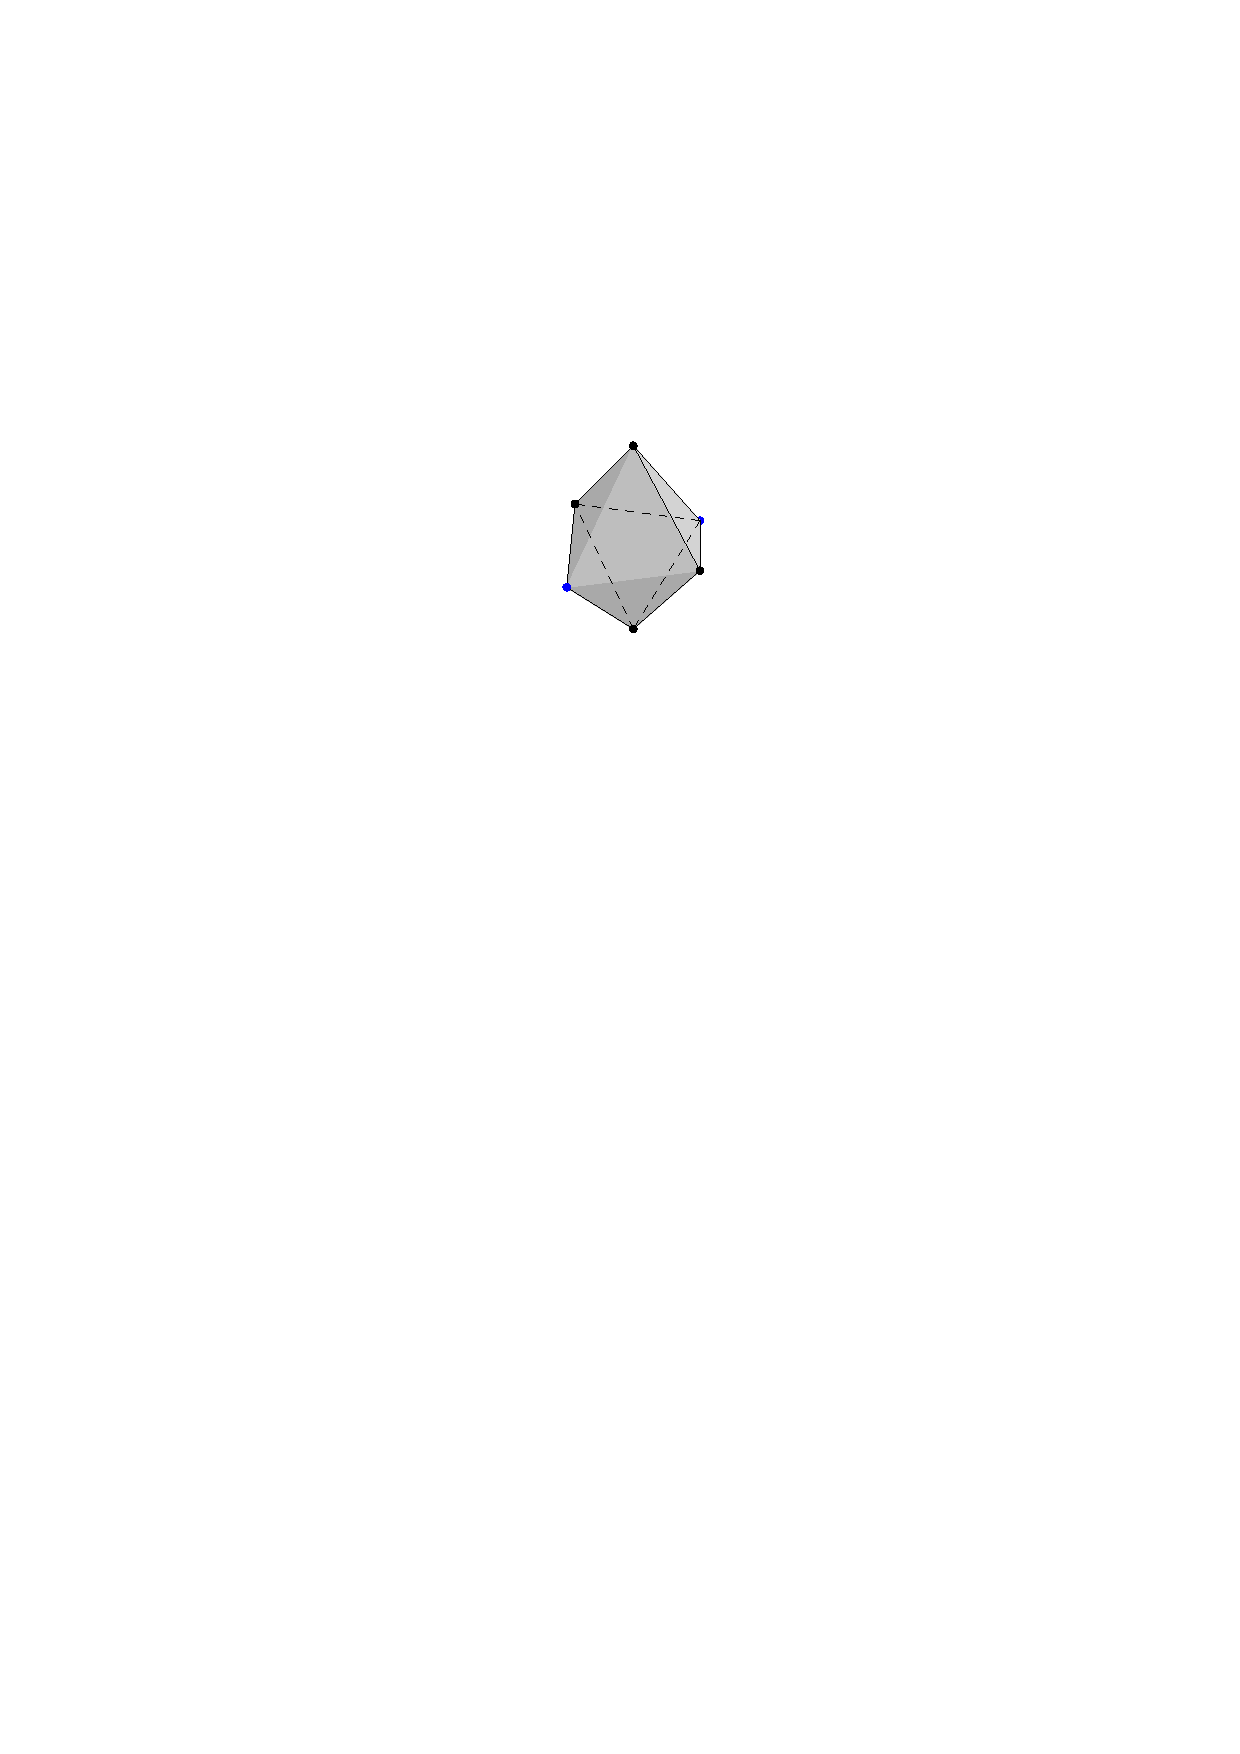
\includegraphics[width=0.25\textwidth]{Figures/threed-qeset.pdf}
	\caption{A dual polytope~$\Qe$ in three dimensions; the two vertices~$v$ and~$w$ are in blue and the extremal points of~$H_e$ are in black.}
	\label{fig:threed-qe}
\end{figure}

\begin{figure}
	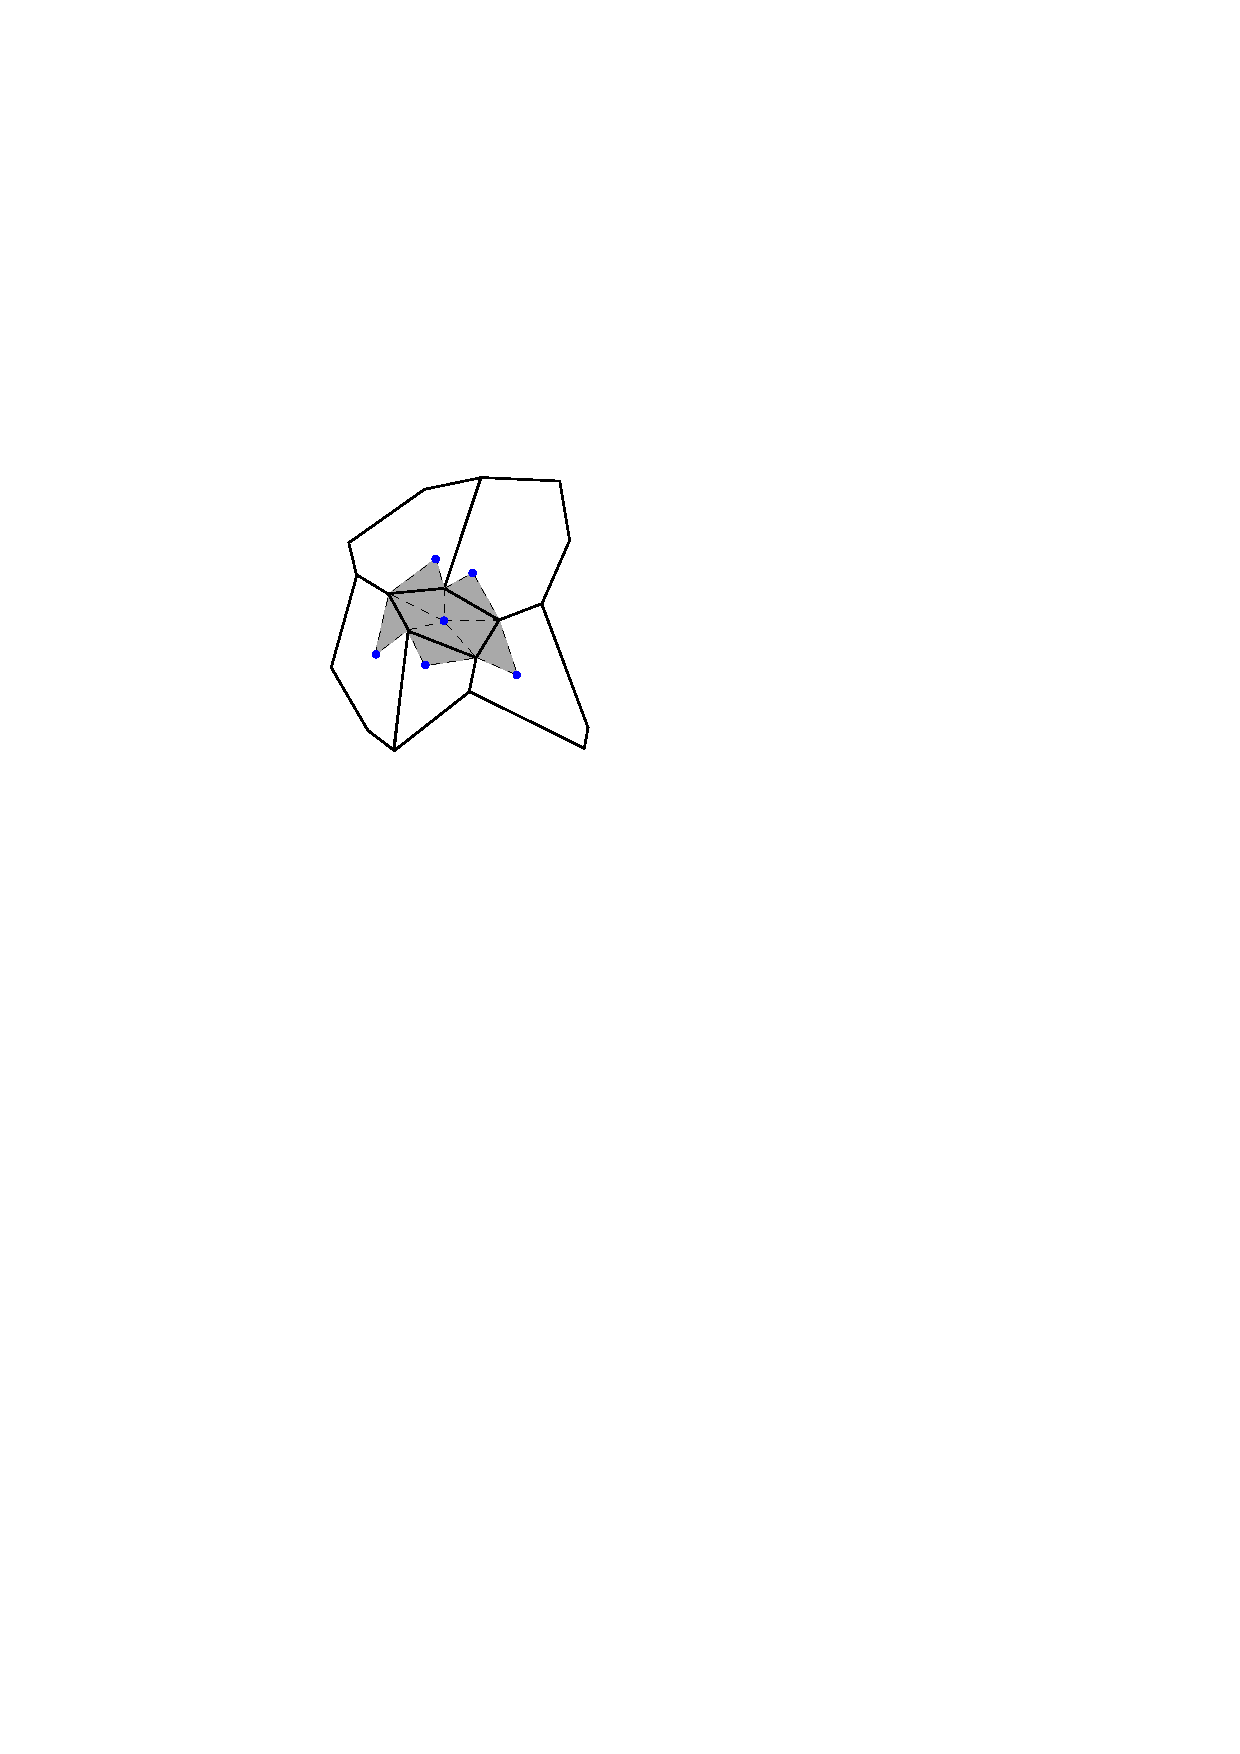
\includegraphics[width=0.25\textwidth]{Figures/qsets-nongab.pdf}
	\caption{A polytope and its neighbors are outlined in thick black and the vertices are blue dots. For each neighbor, the corresponding~$\Qe$ sets are outlined in dashed lines and filled in dark gray.}
	\label{fig:twod-qe}
\end{figure}




We consider the \emph{dual polytope} associated with the edge~$e = (w,v) \in \E$, 
\begin{equation}
	\label{eq:qeset}
\Qe := \conv( w, P_w \cap P_v) \cup \conv(v, P_w \cap P_v)   \, . 
\end{equation}
See Figures~\ref{fig:threed-qe} and~\ref{fig:twod-qe}.
This set appears in our arguments below and we will need to compute its volume. 
The following elementary identity may be deduced from~\cite[Lemma B.2]{droniou2018gradient} but we include a proof for convenience. 

	\begin{figure}
	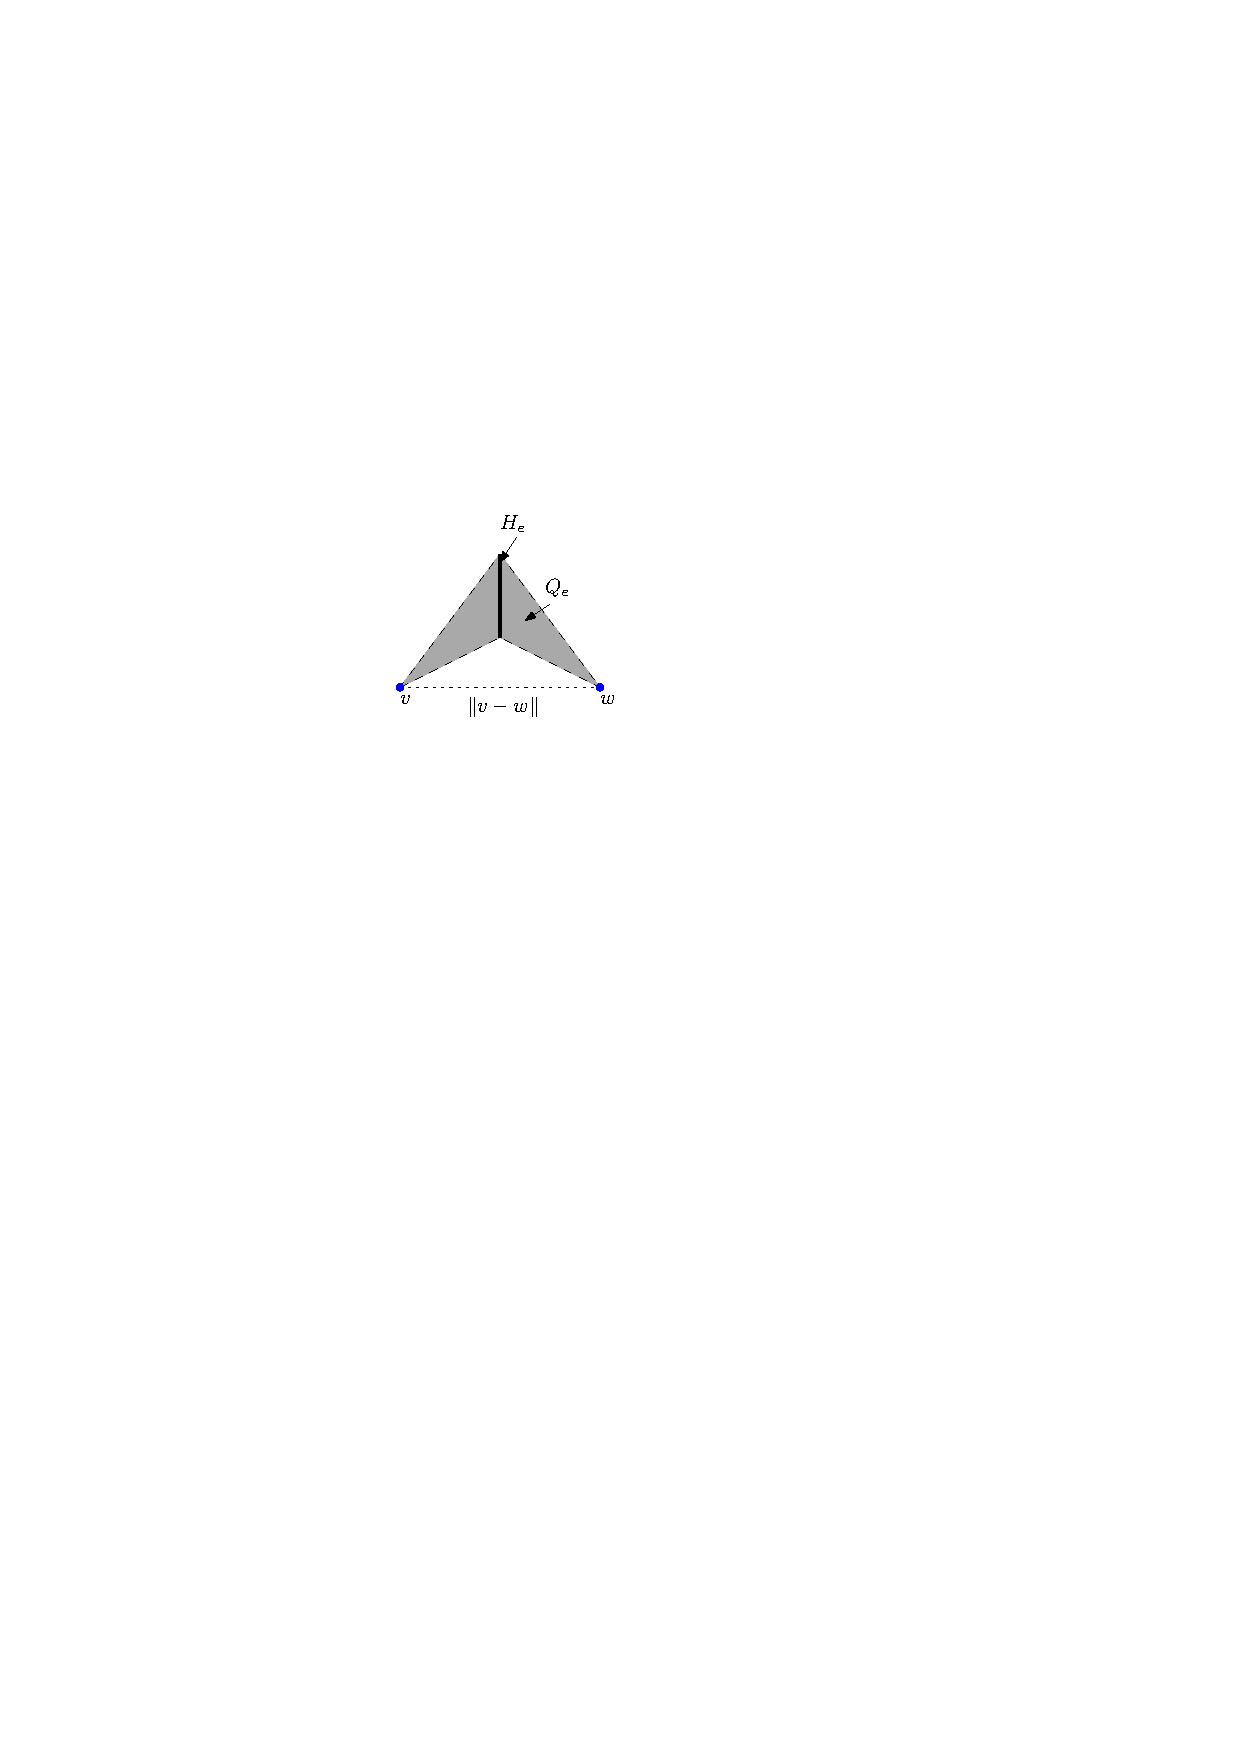
\includegraphics[width=0.25\textwidth]{Figures/non-gabriel-integrate.pdf}
	\caption{Visual aid to computing the volume of~$\Qe$ in the proof of Lemma~\ref{lemma:geometry-bound}. The points~$v,w$ are in blue, the set~$\Qe$ is in light gray outlined by dashed lines, the facet~$H_e$ is a thick black line, and the line between~$v$ and~$w$ is dotted black.}
	\label{fig:non-gabriel-integrate}
\end{figure}
\begin{lemma} \label{lemma:geometry-bound}
	For each edge~$e = (w,v) \in \E$ we have that 
	\[
	 \|w - v\| \vol_{d-1}(H_e)  = d  \vol_d(\Qe) \, . 
	\]
\end{lemma}
\begin{proof}
% CORRECTION 6: Allow the translation needed for the coordinate reduction.
	By a translation and an orthogonal transformation, we may assume that the facet~$H_e$ lies on the hyperplane~$x_1 = 0$
	and that~$w = (w_1, 0, \ldots, 0)$ and~$v = (-v_1, 0, \ldots, 0)$ for~$v_1, w_1 > 0$. In particular, we have
	\[
	 \conv(w, H_e) = \{ \theta x + (1-\theta) w \quad  \mbox{such that~$x \in H_e$ and~$\theta \in [0,1]$}\} \, . 
	\]
	See Figure~\ref{fig:non-gabriel-integrate}.

% CORRECTION 6: Use the correct parametrization of a contact pyramid.
			Identify $H_e$ with a subset of $\R^{d-1}$ in the plane $x_1=0$. The parametrization
        $\phi(t,x)=((1-t)w_1,tx)$, $0<t<1$, has absolute Jacobian $w_1t^{d-1}$. It is one-to-one on the interiors and covers $\conv(w,H_e)$ up to sets of measure zero. Thus
        \[
        \vol_d(\conv(w,H_e))
        =\int_0^1\int_{H_e}w_1t^{d-1}\,d\vol_{d-1}(x)\,dt
        =\frac{w_1}{d}\vol_{d-1}(H_e).
        \]
Similarly, we have that 
	\[
	\vol_{d}(\conv(v, H_e)) = \frac{1}{d} v_1 \vol_{d-1}(H_e) \, . 
	\]
	The previous two displays yield the claim. 
\end{proof}




We will also need to compare the~$d$-dimensional volumes of sets of polytopes which intersect~$U$.
\begin{lemma} \label{lemma:easy-global-qe-bounds}
	 Recall the definition of $\GCU$ for $U\subset \mathcal{D}$ from~\eqref{eq:graph-closure}. For every bounded set~$U \subset \mathcal{D}$
	\begin{equation}
		\label{eq:easy-bounds-geometric-sets}
% CORRECTION 7: The dual cells cover selected cells, rather than an arbitrary domain.
	   \bigcup_{v\in\V[U]}P_v \subset \bigcup_{e \in \E[\overline{U}]} \Qe \subset \GCU \, . 
\end{equation}
%	Moreover, if~$U$ is Lipschitz,  there exist constants~$C = C(d) > 0$ and~$\delta_0 = \delta_0(U, d) > 0$ such that with 
%	\[
%	\delta := \max_{v \in \overline{\mathcal{B}} } \left( \diam(P_v) \right)  \quad \mbox{where} \quad  \mathcal{B} := \{ v \in \V : P_v \cap \partial U \neq \emptyset \}
%	\]
%	we have, for all~$\delta< \delta_0$, the upper bound
%	\begin{equation}
%		\label{eq:boundary-layer-bound}
%	\vol_{d}(\GCU) \leq \vol_{d}(U) + C \delta \vol_{d-1}(\partial U)  \, . 
%	\end{equation}
\end{lemma}

\begin{proof}
	
	
% CORRECTION 7: Supply the facet coverage and disjointness used by the volume estimates.
For $x\in P_v\setminus\{v\}$, extend the ray from $v$ through $x$ to its first point $z$ on $\partial P_v$. Completeness gives a neighbour $w$ with $z\in H_{(w,v)}$, so $x\in\conv(v,H_{(w,v)})$. The marked point $v$ belongs to any such pyramid. This proves the first inclusion, and convexity of each cell proves the second. Distinct contact pyramids in a cell have disjoint interiors: the ray from the marked point meets only one relative interior of a contact, except on finitely many lower dimensional cones. Pyramids in different cells also have disjoint interiors. Consequently, for any set of incident edges,
\[
 \sum_e d\vol_d(Q_e)\leq d\vol_d\left(\bigcup_e Q_e\right)\leq d\vol_d(\widehat U).
\]
The first inequality is in fact an equality. These assertions apply to arbitrary sets of complete active cells, whether or not their union is a domain. Infinite families follow by countable additivity: there are at most countably many cells, since their disjoint nonempty interiors contain distinct rational points. 
%To prove~\eqref{eq:boundary-layer-bound} we first observe that 
%\[
%\GCU \setminus U \subset \bigcup_{v \in \overline{\mathcal{B}}} P_v
%\]
%and 
%\[
%\bigcup_{v \in \overline{\mathcal{B}}} P_v \subset \{ x \in \Rd:  \inf_{y \in \partial U} \|x-y\| < 4 \delta \} \, . 
%\]
%Since~$U$ is Lipschitz, by Weyl's tube formula (see, for example~\cite[Theorem 51]{morvanbook}) there exists a constant~$C(d)$ and~$\delta_0(U, d)$
%such that for all~$\delta < \delta_0$, 
%\[
%\vol_{d} \left( \{ x \in \Rd:  \inf_{y \in \partial U} \|x-y\| < 4 \delta \} \right)\leq  C \delta \vol_{d-1}(\partial U)  \, .
%\]
%Combining the previous three displays completes the proof. 
\end{proof}




% CORRECTION 8: Include only the finite Taylor remainders actually needed by the proofs.
\subsection{Convergence of the energy}
For a finite set of active vertices $A=\V[U]$, write
\[
 K_U:=\widehat U\ \cup\!\!\bigcup_{\{v,w\}\in\E[\overline U]}[v,w].
\]
For $h\in C^2(\widehat U)$ define the finite Taylor remainder constant
\begin{equation}\label{eq:taylor-constant}
 \begin{split}
 T_U(h)&:=\max_{v\in A,\,w\sim v}
 \frac{2|h(w)-h(v)-\Cnabla h(v)\cdot(w-v)|}{\|w-v\|^2},\\
 M_U(h)&:=\max\left\{\sup_{\widehat U}|\Cnabla^2h|,T_U(h)\right\}.
 \end{split}
\end{equation}
The maximum defining $T_U$ uses both orientations of internal edges, and only the active endpoint of a boundary edge. Here $C^2(\widehat U)$ means a $C^2$ extension to an open neighbourhood of the cell union; harmonicity is required only on that union. Hessian norms are operator norms. No values on the added segments of $K_U$ are required. If a $C^2$ extension to $K_U$ has Hessian norm at most $M$, Taylor's theorem gives $M_U(h)\leq M$. More generally the proofs need only the finite inequalities
\begin{equation}\label{eq:finite-taylor-condition}
 |h(w)-h(v)-\Cnabla h(v)\cdot(w-v)|\leq\tfrac M2\|w-v\|^2
 \quad(v\in A,\ w\sim v),
\end{equation}
together with the cell Hessian bound by $M$; $M_U(h)$ is the least such constant. The definitions and estimates apply to any finite active set, by replacing $\V[U]$ by that set.
% CLOSE 1: The quantitative theorems need finite Taylor control only on internal edges.
For the three quantitative theorems we use the smaller constant
\begin{equation}\label{eq:internal-taylor-constant}
\begin{split}
 M_0(h)&:=\sup_{\widehat U}|\Cnabla^2h|,\\
 T_U^\circ(h)&:=\max_{\substack{v,w\in A\\v\sim w}}
 \frac{2|h(w)-h(v)-\Cnabla h(v)\cdot(w-v)|}{\|w-v\|^2},\\
 M_U^\circ(h)&:=\max\{M_0(h),T_U^\circ(h)\}.
\end{split}
\end{equation}
The internal maximum uses both orientations and is zero when there are no internal edges. All estimates are valid with a larger constant than the one specified in their statements. Propositions~\ref{prop:energy-bound} and~\ref{prop:energy-poincare-bound} retain $M_U$; they need~\eqref{eq:finite-taylor-condition} only at one active endpoint of each edge of $\E[\overline U]$, with the Hessian bound on the cell of that endpoint. Theorems~\ref{theorem:2d}, \ref{theorem:generaldim}, and~\ref{theorem:generaldim-decay} use $M_U^\circ$; their proofs below remove every boundary-edge Taylor test. A $C^2$ extension with Hessian bounded by $M$ on the cells and the internal edge segments suffices for $M_U^\circ\le M$. Such uniform control is supplied by the fixed harmonic neighbourhood in the applications. These revised quantitative statements do not assert the corresponding estimates with $M_0$ alone. The counterexamples to the two propositions below are not asserted to disprove those stronger theorem statements.
 
Given a subset of vertices~$A$ with~$\overline{A} \subset \V$ and a function~$f: \overline{A} \to \R$, the~\emph{Dirichlet energy}
of~$f$ is defined as 
 \begin{equation} \label{eq:dir.energy}
	\D(f, A) :=  \sum_{e \in \E[\overline{A}]} \cond(e)^{-1} |\anabla f(e)|^2  \, . 
\end{equation} 
When~$U \subset \Rd$, we write
\[
\D(f, U) := \D(f, \V[U]) \,. 
\]
This definition of energy may also be thought of as 
% CORRECTION 4: The quadratic energy is the square of a seminorm.
the square of a discrete Sobolev seminorm adapted to the geometry of the orthogonal tiling graph, see, \eg,~\cite[Definition 9.3]{eymard2000finite}.

We show the energy of the difference of a continuum harmonic function and its discrete harmonic extension is small. This is well known in the finite volume literature, see for example,~\cite[Theorem 9.3]{eymard2000finite}.
\begin{prop}
	\label{prop:energy-bound}
	Let~$U$ be a bounded domain with~$\overline{U} \subset \mathcal{D}$ and suppose that~$h_C \in C^{2}(\GCU)$ satisfies~$\CLap h_C = 0$ on~$\GCU$ and let~$h_D: \overline{\V[U]} \to \R$ solve 
	\[
	\left\{
	\begin{aligned}
		&  \aDelta h_D = 0 & \mbox{in} & \ \V[U] \,,
		\\
		& h_D = h_C & \mbox{on} & \  \partial \V[U] \, . 
	\end{aligned}
	\right.
	\]
	Then, with
	\[
	\eps := \sup_{v \in \overline{\V[U]}} \diam(P_v)
% CORRECTION 8: Control the cell Hessian and finite edge Taylor remainders by one constant.
	\quad \mbox{and} \quad M := M_U(h_C) 
	\]
	we have the bound
	\begin{equation}
		\label{eq:dirichlet-energy-convergence-bound}
	\D(h_D - h_C, U) \leq 9  M^2 \eps^2 \sum_{e \in \E[\overline{U}]} d \vol_{d}(\Qe)   \, .
	\end{equation}
\end{prop}
\begin{proof}
	Consider the vector field~$\tilde \theta: \E[\overline{U}] \to \R$ defined by 
	\[
	\tilde \theta(w,v) = \int_{P_w \cap P_v} \frac{\Cnabla h_C(y) \cdot (w-v)}{\|w - v\|} \dvol_{d-1}(y)  \qquad \forall (w,v) \in \E[\overline{U}] \, ,
	\]
	and observe that, by the divergence theorem, for every~$v \in \V[U]$ 
	\begin{align*}
	(\div \tilde \theta)(v) &= \sum_{(w,v) \in \E} \tilde \theta(w,v) \\
	&= \sum_{(w,v) \in \E} \int_{P_w \cap P_v} \frac{\Cnabla h_C(y) \cdot (w-v)}{\|w - v\|}  \dvol_{d-1}(y)
	= \int_{P_v}\CLap h_C(x) \dvol_{d}(x)= 0 \, . 
	\end{align*}
	Define the vector field~$\theta: \E[\overline{U}] \to \R$ by
	\[
	\theta(w,v) := \tilde \theta(w,v) - \anabla h_C(w,v)  \quad \forall (w,v) \in \E[\overline{U}] \, . 
	\]
	Let~$f := h_D - h_C$ and observe that by the above two displays and the fact that~$h_D$ is discrete harmonic, we have that on~$\V[U]$, 
	\[
	\div(\theta) = \div(- \anabla h_C) = \div(\anabla h_D - \anabla h_C) =  \div(\anabla f) \, . 
	\]
	Consequently, since~$f$ is zero on~$\partial \V[U]$, we have by Lemma~\ref{lemma:dual-variational-principle} that
	\begin{equation}
		\label{eq:bound-on-d-by-flow}
	\D(f, U) \leq \sum_{e \in \E[\overline{U}]} \cond(e)^{-1} \theta(e)^2 \, , 
\end{equation}
	and so it suffices to bound the sum on the right. By definition of~$\anabla f$ we have 
	\begin{align*}
	\theta(w,v)  %&= \int_{P_w \cap P_v} \frac{\Cnabla h_C \cdot (w-v)}{\|w - v\|} - \anabla h_C \\
	&= \int_{P_w \cap P_v} \frac{\Cnabla h_C(y) \cdot (w-v) - (h_C(w) - h_C(v))}{\|w - v\|} \dvol_{d-1}(y) \, ,
	\end{align*}
	and so 
	\begin{align}
	&\cond(w,v)^{-1} \theta(w,v)^2  \notag \\
	&= \|w-v\| \vol_{d-1}(P_w \cap P_v) \times  \notag \\
	&\qquad  \left( \frac{1}{\vol_{d-1}(P_w \cap P_v)} \int_{P_w \cap P_v} \frac{\Cnabla h_C(y) \cdot (w-v) - (h_C(w) - h_C(v))}{\|w - v\|} \dvol_{d-1}(y) \right)^2  
	\label{eq:bound-on-conductance}
	\, . 
	\end{align}
% CORRECTION 8: Use the finite Taylor condition without assuming an extension along the segment.
For each undirected incident edge choose an endpoint $v\in\V[U]$. By~\eqref{eq:finite-taylor-condition} we have
	\[
% CORRECTION 8: Take the Taylor expansion at the active endpoint.
	|h_C(w) - (h_C(v) + \Cnabla h_C(v) \cdot (w - v))| \leq \frac{M}{2} \|w-v\|^2 
	\]	
	and the mean value inequality, 
	\[
	|(\Cnabla h_C(y) - \Cnabla h_C(y')) \cdot (w-v) | \leq M \ \|y-y'\| \  \|w-v\|  
% CORRECTION 8: Compare gradients inside one convex cell.
\qquad \forall y,y' \in P_v \, . 
	\]
	The previous two displays and the triangle inequality yield 
	\begin{equation}
	\label{eq:bound-on-flux-difference}
	\sup_{y \in P_w \cap P_v} \frac{|\Cnabla h_C(y) \cdot (w-v) - (h_C(w) - h_C(v))|}{\|w - v\|} \leq 3 M \eps \, . 
	\end{equation}	
	Combining~\eqref{eq:bound-on-d-by-flow},~\eqref{eq:bound-on-conductance}, and~\eqref{eq:bound-on-flux-difference} with Lemma~\ref{lemma:geometry-bound} completes the proof.
\end{proof}


\section{Iterating to get a pointwise bound} 
\label{sec:iteration}
In this section we prove Theorem~\ref{theorem:convergence-of-the-dirichlet-problem} under Hypothesis~\ref{item:cont-neighborhood}. We start by converting the energy estimate (Proposition~\ref{prop:energy-bound}) into a pointwise bound on columns (Proposition~\ref{prop:energy-poincare-bound})
using a Poincar\'e-type bound (Lemma~\ref{lemma:ptype-inequality}).

We then observe that this leads, by planarity, to a short proof when~$d=2$ (Theorem~\ref{theorem:2d}).
In higher dimensions, we use Hypotheses~\ref{item:vol} or~\ref{item:diam}
together with an iteration to prove the claims in Theorems~\ref{theorem:generaldim} or~\ref{theorem:generaldim-decay} respectively.


\subsection{Pointwise bound on columns}
\begin{figure}
	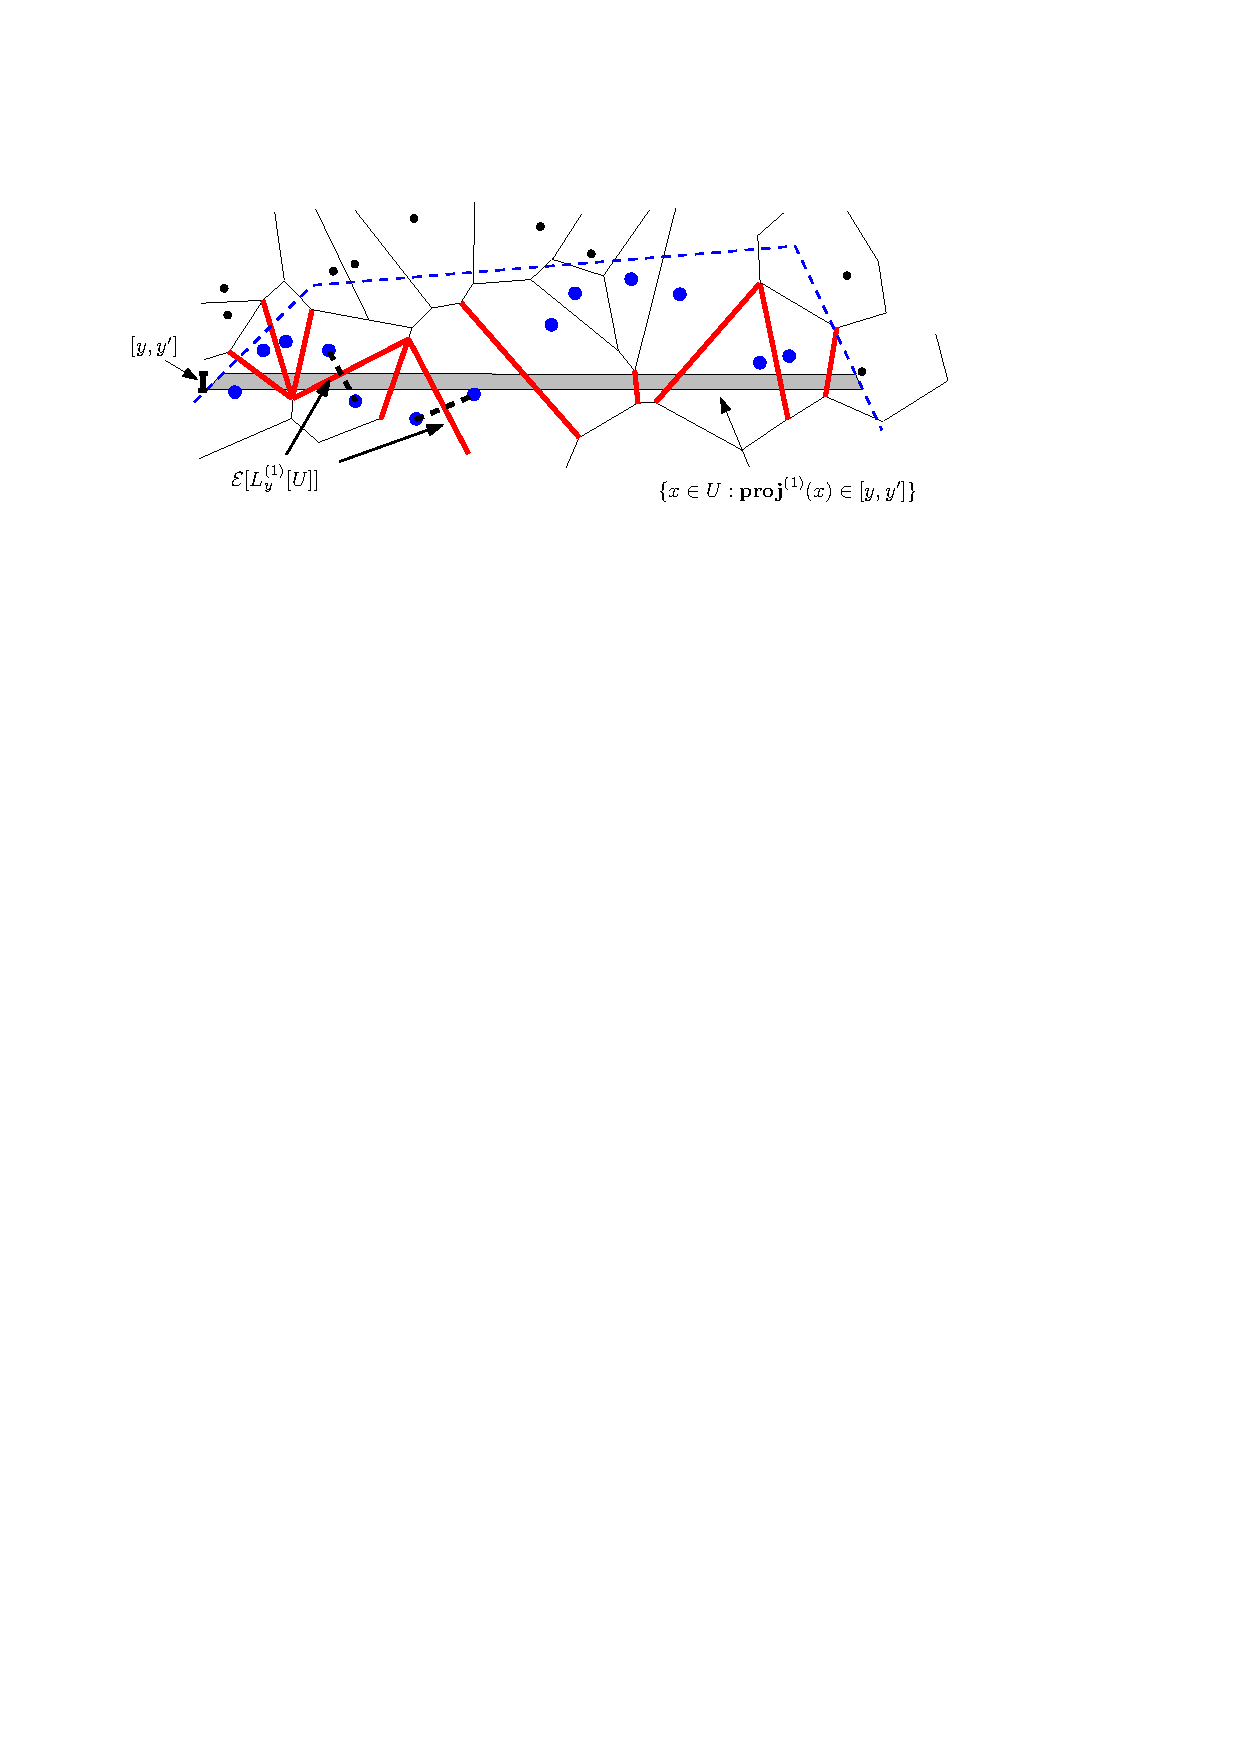
\includegraphics[width=0.7\textwidth]{Figures/induced-poincare.pdf}
	 \caption{Part of Figure~\ref{fig:induced-subgraph} is shown along with
		(red) facets which have projections intersecting a small (gray) interval~$[y,y']$. Two edges in~$\E[\Lyone[U]]$ are displayed.} 
			\label{fig:project-lines}
\end{figure}



We record a bound obtained from the proof of the Poincar\'e inequality. The discrete Poincar\'e inequality which this leads
to may be found in~\cite[Lemma 9.1]{eymard2000finite}. 


For~$x \in \Rd$ and~$j \in \{1, \ldots, d\}$ we write~$\projj(x)  = (x_1, \ldots, x_{j-1}, x_{j+1}, \ldots, x_d)$ for the orthogonal projection of~$x$ onto~$\R^{d-1}$ obtained by removing the~$j$th coordinate. For a domain~$U \subset \Rd$,~$j \in \{1, \ldots, d\}$, and~$y \in \R^{d-1}$, we write
\begin{equation}
	\begin{aligned}
	\label{eq:line-project}
	\E[\Lyj[U]] &= \{ e \in \E[\overline{U}] : y \in \projj(H_e) \} \\
	\Lyj[U] &= \{v \in \V[U]: v \mbox{ is an endpoint of~$e$ for some~$e \in \E[\Lyj[U]]$} \} \, ,
	\end{aligned} 
\end{equation}
for the set of edges (resp. endpoints of edges) adjacent to~$U$ with projected facets which intersect~$y$ --- see Figure~\ref{fig:project-lines}. 
Note that there can be edges in~$\E[\Lyj[U]]$ whose projections do not contain $y$.




\begin{lemma}[Poincar\'e-type inequality]
	\label{lemma:ptype-inequality}
	For every bounded domain~$U$ with~$\overline{U} \subset \mathcal{D}$, coordinate~$j \in \{1, \ldots, d\}$, and 
% CORRECTION 9: The zero boundary condition requires a function on the graph closure.
function~$f: \overline{\V[U]} \to \R$ which is zero on~$\partial \V[U]$ we have for every~$k > 0$
	\[
	\vol_{d-1}\left( y \in \projj(U): \max_{v \in \Lyj[U]} |f(v)| > k    \left( \D(f,U) \sum_{e \in \E[\overline{U}]} d   \vol_{d}(\Qe) \right)^{\! \!  \! \!\nicefrac12} \right) \leq k^{-1}  \, . 
	\]
\end{lemma}
\begin{proof}

	
	By interchanging summation and integration, 
	\[
		\int_{\projj(U)} \sum_{e \in \E[\Lyj[U]]} |\nabla^{\mathcal{G}} f(e)| \dvol_{d-1}(y)
		 \leq \sum_{e \in \E[\overline{U}]} |\nabla^{\mathcal{G}} f(e)| \vol_{d-1}(H_e)  \, . 
	\]
	Consequently, by the Cauchy–Schwarz inequality, 
	\begin{align*}
		&\int_{\projj(U)} \sum_{e \in \E[\Lyj[U]]} |\nabla^{\mathcal{G}} f(e)| \dvol_{d-1}(y) \\
		&\leq  \sqrt{\sum_{e \in \E[\overline{U}]} |\nabla^{\mathcal{G}} f(e)|^2 \cond(e)} \sqrt{ \sum_{e \in \E[\overline{U}]}    \cond^{-1}(e) \vol_{d-1}(H_e)^2	} \\
		&=  \sqrt{\sum_{e \in \E[\overline{U}]}  |\nabla^{\mathcal{G}} f(e)|^2 \cond(e)} \sqrt{ \sum_{e \in \E[\overline{U}]}   d \vol_{d}(\Qe)	} \, , 
	\end{align*}
	where in the last equality we used Lemma~\ref{lemma:geometry-bound}. This implies
	\begin{equation}
		\label{eq:bound-on-sums-of-gradients}
		\int_{\projj(U)} \sum_{e \in \E[\Lyj[U]]} |\nabla^{\mathcal{G}} f(e)| \dvol_{d-1}(y) \leq   \D(f,U)^{\nicefrac12}   \left( \sum_{e \in \E[\overline{U}]} d   \vol_{d}(\Qe)  \right)^{\! \!  \! \!\nicefrac12} \, . 
	\end{equation}
% CORRECTION 9: A generic line gives separate paths to the boundary, not one connected column.
			For almost every line parallel to the $j$th axis, its intersections with the finitely many active cells avoid all contacts of dimension at most $d-2$ and all facets parallel to the line. Each nonempty intersection with a cell is an interval of positive length. Starting in any active cell met by this line and following the line in the positive direction, completeness gives a succession of neighbouring cells until the line leaves the finite union of active cells. The last crossing leads to a vertex of $\partial\V[U]$, where $f=0$. Telescoping along this path gives
        \[
        \max_{v:\,y\in\projj(P_v),\ v\in\V[U]}|f(v)|
        \leq\sum_{e\in\E[\Lyj[U]]}|\nabla^{\mathcal G}f(e)|.
        \]
        Different components of the line's intersection with the active cells are treated separately; they need not be connected to one another. Empty maxima are zero. The same calculation as above, integrated over all $\R^{d-1}$, gives
        \[
        \int_{\R^{d-1}}\max_{v:\,y\in\projj(P_v),\ v\in\V[U]}|f(v)|\,dy
        \leq\left(\D(f,U)\sum_{e\in\E[\overline U]}d\vol_d(Q_e)\right)^{1/2}.
        \]
        This also proves the stronger version with the whole projection space in place of $\projj(U)$.

By the above two displays and Chebyshev's inequality, we have that, for all~$\delta> 0$
	\[
	\vol_{d-1} \left( y \in \projj(U): \max_{v \in \Lyj[U]} |f(v)| > \delta \right) \leq \delta^{-1}  \D(f,U)^{\nicefrac12}   \left( \sum_{e \in \E[\overline{U}]} d   \vol_{d}(\Qe)  \right)^{\! \!  \! \!\nicefrac12}  \, . 
	\]
	This completes the proof. 
\end{proof}



By combining the above inequality together with Proposition~\ref{prop:energy-bound} we obtain a pointwise bound on the 
difference between the discrete and continuous harmonic functions on an arbitrarily dense set of columns. 
\begin{prop}[Closeness on columns]
	\label{prop:energy-poincare-bound}
	Let~$U$ be a bounded domain with~$\overline{U} \subset \mathcal{D}$ and suppose that~$h_C \in C^{2}(\GCU)$ satisfies~$\CLap h_C = 0$ on~$\GCU$ and let~$h_D: \overline{\V[U]} \to \R$ satisfy 
	\[
	\left\{
	\begin{aligned}
		&  \aDelta h_D = 0 & \mbox{in} & \ \V[U] \,,
		\\
		& h_D = h_C & \mbox{on} & \  \partial \V[U] \, . 
	\end{aligned}
	\right.
	\]
	Then, with
	\[
	\eps := \sup_{v \in \overline{\V[U]}} \diam(P_v)
% CORRECTION 8: Control the cell Hessian and finite edge Taylor remainders by one constant.
	\quad \mbox{and} \quad M := M_U(h_C)
	\]
	we have for every~$k > 0$ and~$j \in \{1, \ldots, d\}$,
	\[
	\vol_{d-1} \left( y \in \projj(U): \max_{v \in \Lyj[U]} |h_D(v) - h_C(v)| > 3 k M \eps \sum_{e \in \E[\overline{U}]} d   \vol_{d}(\Qe)  \right) \leq k^{-1}  \, . 
	\]
\end{prop}
\begin{proof}
% CORRECTION 9: Record the full-projection version actually supplied by the line argument.
	This is immediate from Lemma~\ref{lemma:ptype-inequality} and Proposition~\ref{prop:energy-bound}. The same estimate holds with $\R^{d-1}$ in place of $\projj(U)$, and with columns defined by $y\in\projj(P_v)$, by the full-projection version proved above. 
\end{proof}

% CORRECTION 8: Give a direct counterexample to both cell-only analytic bounds.
\smallskip
\noindent\emph{The cell-only Hessian hypotheses in Propositions~\ref{prop:energy-bound} and~\ref{prop:energy-poincare-bound} do not suffice.}
Here is one counterexample to both, with all cells complete. For small $\alpha>0$ put $\beta=\alpha/3$ and $r_t=(\sin t,\cos t)$. Take sites $r_{-\alpha},r_{-\beta},r_\beta,r_\alpha$, their multiples by $5$, and $(0,\pm5)$. Denote the first four sites by $v,y,z,w$, respectively. Clip their Voronoi diagram to
\[
 Q_\alpha=[-10\alpha,10\alpha]\times[-50,50],
\]
and reflect the entire site pattern repeatedly across its sides. This gives a locally finite Voronoi tiling of $\R^2$ with bounded complete cells. Indeed inside $Q_\alpha$ each reflected site is no closer than its original progenitor, while each site's own reflections constrain its cell to this box. Thus the original cells are precisely the clipped cells.

Comparing squared distances, the facet $v|w$ is the downward ray from zero, of length $12/(5+\cos\alpha)$, and $v|y$ is the upward ray in direction $r_{-2\beta}$, of length $3/\cos\beta$. They are not cut by the vertical sides. The left side of $P_v$ has endpoints whose second coordinates tend to $-2$ and $3$ and length tending to $5$; across it the neighbour is $v^-=(-20\alpha+\sin\alpha,\cos\alpha)$. The cell does not meet the other box sides. Consequently
\[
 \alpha\cond(v,w)\to1,\qquad
 \alpha\cond(v,y)\to9/2,\qquad
 \alpha\cond(v,v^-)\to5/18.
\]
These follow by dividing the three facet lengths by $2\sin\alpha$, $2\sin\beta$, and $20\alpha-2\sin\alpha$, respectively. All other neighbours are original sites of norm $5$, so their edge lengths are at least $4$ and their conductances stay bounded.

The radial ray $\Gamma_\alpha=\{t r_\beta:t\geq1/4\}$ misses $P_v$ and all its neighbour cells. Inside the box its nearest sites are only $z$ and $5z$, changing at $t=3$. The cells of $v,z$ meet only at zero: their upper bisector is dominated by $y$ and their lower bisector by $w$. The cells of $v,5z$ are disjoint: membership in $P_v$ gives $x_1\leq0$ and $x_1\leq-x_2\tan(2\beta)$, while membership in $P_{5z}$ gives $x\cdot r_\beta\geq3$, forcing $x_2>0$ and then $x_1<0$. The site $5y$ is strictly closer than $5z$ there. The ray leaves the box through its right side at height tending to $30$ and thereafter lies to its right. The only neighbour of $v$ in another reflected box is $v^-$, whose cell lies to the left. This proves the assertion about the cut.

Set $c_\alpha=r_\beta/4$ and, on $\C\setminus\Gamma_\alpha$, define
\[
 h_\alpha(\zeta)=\Re\left[\frac4{15\sqrt{200}}(\zeta-c_\alpha)^{5/2}\right],
 \quad\arg(\zeta-c_\alpha)\in(\pi/2-\beta,\pi/2-\beta+2\pi).
\]
This is smooth and harmonic near the union of $P_v$ and its neighbour cells. That union lies in $[-30\alpha,10\alpha]\times[-50,50]$, so its Hessian operator norm, equal to $\sqrt{|\zeta-c_\alpha|/200}$, is at most $1$ for small $\alpha$. Direct evaluation gives
\[
 \begin{gathered}
 h_\alpha(w)-h_\alpha(v)\to J:=\frac{4\sqrt2}{15\sqrt{200}}(3/4)^{5/2}>0,
 \\
 h_\alpha(y)-h_\alpha(v)=O(\alpha),\quad
 h_\alpha(v^-)-h_\alpha(v)=O(\alpha).
 \end{gathered}
\]
The last two pairs approach the same side of the cut; the first pair approaches opposite sides. All remaining neighbour values stay bounded.

Choose
\[
 U_\alpha=(-\sin\alpha-\alpha/10,-\sin\alpha+\alpha/10)\times(-1/2,3/2).
\]
It contains exactly the site $v$. Its singleton harmonic extension therefore has error
\[
 f(v)=\frac{\sum_{u\sim v}\cond(v,u)(h_\alpha(u)-h_\alpha(v))}
                 {\sum_{u\sim v}\cond(v,u)}\longrightarrow\frac9{52}J>0.
\]
Meanwhile $\eps\leq105$ and, by disjointness of dual interiors,
$\Sigma_\alpha:=\sum_{e\in\E[\overline U_\alpha]}2\vol_2(Q_e)\leq2\vol_2(\widehat U_\alpha)\leq8000\alpha$.
The energy is $f(v)^2\sum_{u\sim v}\cond(v,u)$, which diverges like $\alpha^{-1}$, whereas the proposed cell-only energy bound tends to zero. For the column bound take $j=1$, $k=1$. The left facet's projection covers $(-1/2,3/2)$ for small $\alpha$, so every tested column contains $v$. The proposed threshold $3M\eps\Sigma_\alpha$ tends to zero; hence the bad set has length $2$, contradicting the proposed upper bound $1$. Counting both orientations only doubles $\Sigma_\alpha$ and gives the same contradiction.

%We require an elementary geometric fact about the projected sets. 
%\begin{lemma}
%	\label{lemma:sets-equal-to-closure}
%	Let~$U \subset \Rd$ be a bounded domain and let~$f: \overline{\V[U]} \to \R$. For any~$a > 0$, the set
%	\[
%	Y := \{y \in \proj(U): \max_{v \in \Lyj[U]} |f(v)| > a \}
%	\]
%	is a finite union of convex sets and satisfies~$\vol_{d-1}(Y) = \vol_{d-1}(\overline{Y})$.
%\end{lemma}
%\begin{proof}
%	Every point~$y \in Y$ lies on some~$(d-1)$ dimensional facet of a polytope,~$P_w \cap P_v$. Since the polytopes~$P_w,P_v$ are convex, so is the facet~$P_w \cap P_v = H_e$ and its projection~$\proj(H_e)$. As there are only a finite number of polytopes in~$\GCU$, the set~$Y$ is a finite union of convex sets and thus has Lipschitz boundary. This shows that~$\vol_{d-1}(Y) = \vol_{d-1}(\overline{Y})$ 
%\end{proof}
%



\subsection{Two dimensions}
We give a short proof of a strengthened version of the main result in~\cite{gurel2020dirichlet}.
Roughly, when~$d=2$, by taking~$k$ large enough, Proposition~\ref{prop:energy-poincare-bound} guarantees that there is a fine grid of ``good lines'' upon which the discrete and continuous harmonic functions~$h_D$ and~$h_C$ are close. On every rectangle formed by the grid, by smoothness,~$h_C$ is essentially constant. Thus, by the maximum principle,~$h_D$ is close to~$h_C$ everywhere. 
\begin{figure}
	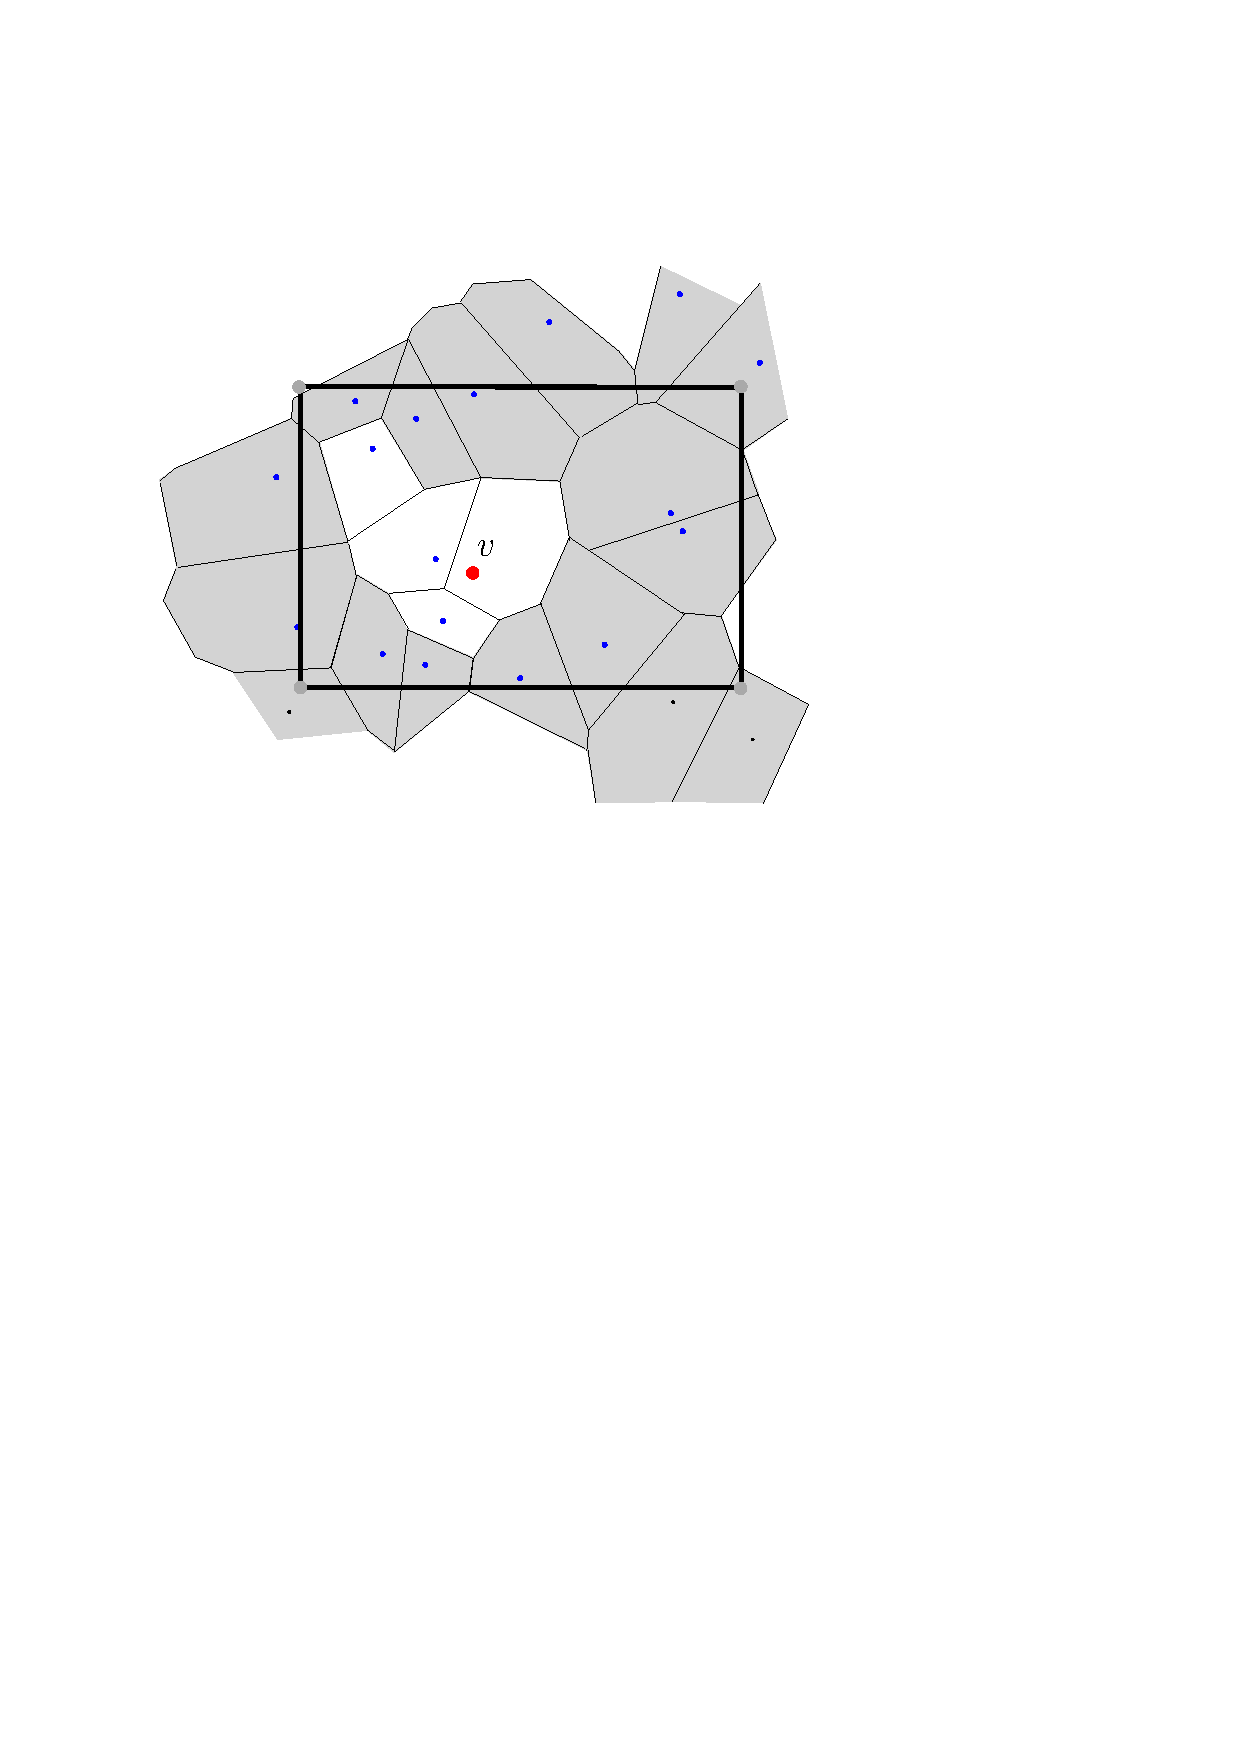
\includegraphics[width=0.5\textwidth]{Figures/small-good-square.pdf}
	\caption{Illustration of the proof of Theorem~\ref{theorem:2d}. The square~$S$ is outlined in black, the cells for which the discrete harmonic function is close to the continuum one are in light gray. }	\label{fig:small-good-square}
\end{figure}

% CLOSE 2: Boundary fluxes have a cell-only bound, permitting internal-edge Taylor control.
\paragraph{Internal-edge comparison.}
The following estimates will be used in all three quantitative theorems. Write $A=\V[U]$, $h=h_C$, $f=h_D-h$, $M_0=M_0(h)$, and $M\ge M_U^\circ(h)$. Use outward-index notation, so $\div\theta(v)=\sum_{w\sim v}\theta_{vw}$, and put
\[
 J_{vw}=\int_{H_{vw}}\Cnabla h(p)\cdot\frac{w-v}{\|w-v\|}\,dp,
 \qquad \theta_{vw}=J_{vw}-\cond(v,w)(h(w)-h(v)).
\]
These are the flux and discrepancy used in Proposition~\ref{prop:energy-bound}; in particular $\div\theta=\aDelta f$ on $A$.
For $p\in H_{vw}$, Taylor expansion at $p$ along the two segments inside $P_v$ and $P_w$ gives
\[
 |h(w)-h(v)-\Cnabla h(p)\cdot(w-v)|
 \le\frac{M_0}{2}\bigl(\|w-p\|^2+\|v-p\|^2\bigr).
\]
Averaging over the contact yields the cell-only bound
\begin{equation}\label{eq:cell-flux-bound}
 \frac{|\theta_{vw}|}{\cond(v,w)}
 \le\frac{M_0}{2}\bigl((\diam P_v)^2+(\diam P_w)^2\bigr).
\end{equation}
Also, integration of $\Cnabla h-\Cnabla h(v)$ along the broken segment $v,p,w$, parametrized by arclength, gives
\begin{equation}\label{eq:broken-taylor-bound}
 |h(w)-h(v)-\Cnabla h(v)\cdot(w-v)|
 \le\frac{M_0}{2}(\diam P_v+\diam P_w)^2.
\end{equation}
Indeed, at arclength $s$ the gradient difference is at most $M_0s$, and the integral of the constant gradient along the path is its scalar product with $w-v$.

For $S\subset A$, put $m(S)=\sum_{e\in\E[\overline S]}d\vol_d(Q_e)$ and let $g_S$ be the zero-boundary solution of
\[
 \aDelta g_S=\div(\theta 1_{\E[S]})\quad\hbox{on }S,
\]
extended by zero to $\overline A$. The source uses only edges with both endpoints in $S$. Every component of a finite set of complete cells has a boundary neighbour, as follows by following a generic line to its last exit. Thus the Dirichlet matrix is positive definite and the solution exists uniquely.
If both endpoints of an internal edge have cells of diameter at most $\delta$, the finite Taylor inequality from~\eqref{eq:internal-taylor-constant} and comparison of gradients in one cell give
\[
 |\theta(e)|/\cond(e)\le (M/2)\|e\|^2+M\delta\|e\|
 \le3M\delta\|e\|.
\]
Together with~\eqref{eq:cell-flux-bound}, this proves
\begin{equation}\label{eq:internal-flux}
 \cond(e)^{-1}\theta(e)^2\le9M^2\delta^2d\vol_d(Q_e),
 \qquad |\theta(e)|/\cond(e)\le M_0\delta^2.
\end{equation}
Lemma~\ref{lemma:dual-variational-principle}, applied to the internal source field, therefore gives
\begin{equation}\label{eq:internal-energy}
 \D(g_S,S)\le9M^2\delta^2m(S)
 \quad\hbox{if }\max_{v\in S}\diam P_v\le\delta.
\end{equation}
We shall repeatedly use the following boundary comparison. If $b=0$ on $\partial S$ and
\[
 |\aDelta b(v)|\le b_0\sum_{w\in\partial S}\cond(v,w),
\]
then $|b|\le b_0$. The function $c=b_0 1_S$, zero on $\partial S$, satisfies
\[
 \aDelta c(v)=-b_0\sum_{w\in\partial S}\cond(v,w).
\]
Thus $b-c$ and $-b-c$ are subharmonic with zero boundary values, proving the assertion by the maximum principle. Apply this to the boundary edges in $f-g_A$, using~\eqref{eq:cell-flux-bound}, to obtain
\begin{equation}\label{eq:initial-boundary-correction}
 \|f-g_A\|_\infty\le M_0\eps^2.
\end{equation}

% CLOSE 3: Replace the local oscillation condition by a quadratic bound and optimize the planar rate.
\begin{theorem}
\label{theorem:2d}
Let $U$ be a bounded domain with $\overline U\subset\mathcal D\subset\R^2$, and let $h_C\in C^2(\widehat U)$ be harmonic on $\widehat U$. Let $h_D$ be discrete harmonic on $A=\V[U]$ with $h_D=h_C$ on $\partial A$. With
\[
 \eps=\max_{v\in\overline A}\diam P_v,\qquad
 M_0=\sup_{\widehat U}|\Cnabla^2h_C|,\qquad M=M_U^\circ(h_C),
\]
we have
\begin{equation}\label{eq:planar-quadratic-close}
 \sup_{v\in A}|h_D(v)-h_C(v)|
 \le3M_0\eps^2+\inf_{k>0}\left\{
 6kM\eps\vol_2(\widehat U)+\frac M2(\sqrt2 k^{-1}+\eps)^2\right\}.
\end{equation}
In particular, for $0<\eps\le1/2$ there exists $C=C(U,M)<\infty$ such that
\[
 \sup_{v\in A}|h_D(v)-h_C(v)|\le C\eps^{2/3}\le C\eps^{1/2}.
\]
No local oscillation condition or Lipschitz condition between vertices is assumed.
\end{theorem}
\begin{proof}
The empty set is covered by the zero conventions. If $M=0$, then~\eqref{eq:cell-flux-bound} gives $\theta=0$, so $f=0$ by uniqueness. Otherwise fix $k>0$, put $g=g_A$ and $t=6kM\eps\vol_2(\widehat U)$. The full-projection inequality in the proof of Lemma~\ref{lemma:ptype-inequality},~\eqref{eq:internal-energy}, and $m(A)\le2\vol_2(\widehat U)$ show that, for $j=1,2$,
\[
 B_j=\bigcup_{v\in A:\ |g(v)|>t}\projj(P_v)
\]
has length at most $k^{-1}$. Each is a finite union of closed intervals. If $|g(v)|>t$, choose cuts outside $B_j$ arbitrarily close to the endpoints of the component containing $\projj(P_v)$. The resulting open rectangle $S$ contains $P_v$ and has diameter at most $\sqrt2 k^{-1}+\eta$, where $\eta>0$ is arbitrary.

Let $Q$ be the graph component of $v$ among $u\in A$ with $P_u\subset S$. Every $w\in\partial Q\cap A$ has a cell meeting a side of $S$: it meets a cell of $Q$ inside $S$, and cannot itself be contained in $S$, since otherwise it would belong to $Q$. The side's cut coordinate is outside the corresponding $B_j$, so $|g(w)|\le t$. On $\partial A$ we have $g=0$. Moreover
\[
 \rho:=\max_{w\in\partial Q}\|w-v\|\le\diam S+\eps,
\]
by choosing a contact point in $S$.

For $u\in A$, write $R_{uw}=h_C(w)-h_C(u)-\Cnabla h_C(u)\cdot(w-u)$. Zero divergence of $J$ and Lemma~\ref{lemma:linear-lie-in-kernel} give
\[
 \aDelta g(u)=-\sum_{w\in A:w\sim u}\cond(u,w)R_{uw}
 +\sum_{w\in\partial A:w\sim u}
 \left(\cond(u,w)\Cnabla h_C(u)\cdot(w-u)-J_{uw}\right).
\]
An internal remainder is at most $(M/2)\|w-u\|^2$. A boundary bracket, divided by its conductance, is at most $M_0\diam(P_u)\|w-u\|\le2M_0\eps^2$, by comparison of gradients on $P_u$. For $q(x)=\|x-v\|^2$, affine harmonicity gives $\aDelta q(u)=\sum_{w\sim u}\cond(u,w)\|w-u\|^2$. Consequently, on $Q$,
\[
 |\aDelta g(u)|\le(M/2)\aDelta q(u)+2M_0\eps^2
                  \sum_{w\in\partial Q}\cond(u,w).
\]
Both $g+(M/2)q-2M_0\eps^2 1_Q$ and $-g+(M/2)q-2M_0\eps^2 1_Q$ are subharmonic, with boundary values at most $t+(M/2)\rho^2$. At $v$ the maximum principle gives
$|g(v)|\le t+(M/2)\rho^2+2M_0\eps^2$. Vertices with $|g(v)|\le t$ satisfy this bound as well. Add~\eqref{eq:initial-boundary-correction}, let $\eta\downarrow0$, and take the infimum over $k$ to prove~\eqref{eq:planar-quadratic-close}.

For the rate take $k=\eps^{-1/3}$. If $U\subset B_{R_0}$ and $\eps\le1/2$, then $\widehat U\subset B_{R_0+1}$, and
\[
 C=M\left(3+6\vol_2(B_{R_0+1})+\tfrac12(\sqrt2+1)^2\right)
\]
works, since $M_0\le M$, $\eps\le\eps^{1/3}$, and $\eps^2\le\eps^{2/3}$.
\end{proof}
% CLOSE 3: Retain the stronger quadratic inequality when the full edge constant is available.
With $M=M_U(h_C)$, the additive term $3M_0\eps^2$ in~\eqref{eq:planar-quadratic-close} can be omitted. Indeed Proposition~\ref{prop:energy-bound} and the full-projection inequality apply directly to $f=h_D-h_C$, so the good rectangles have $|f|\le t$ on their graph boundaries. The Taylor inequalities on every incident edge give $|\aDelta f|\le(M/2)\aDelta q$. Apply the maximum principle to $\pm f+(M/2)q$ in the same rectangles. This retains the unconditional quadratic estimate with the full Taylor constant.



\begin{figure}[!h]
\fbox{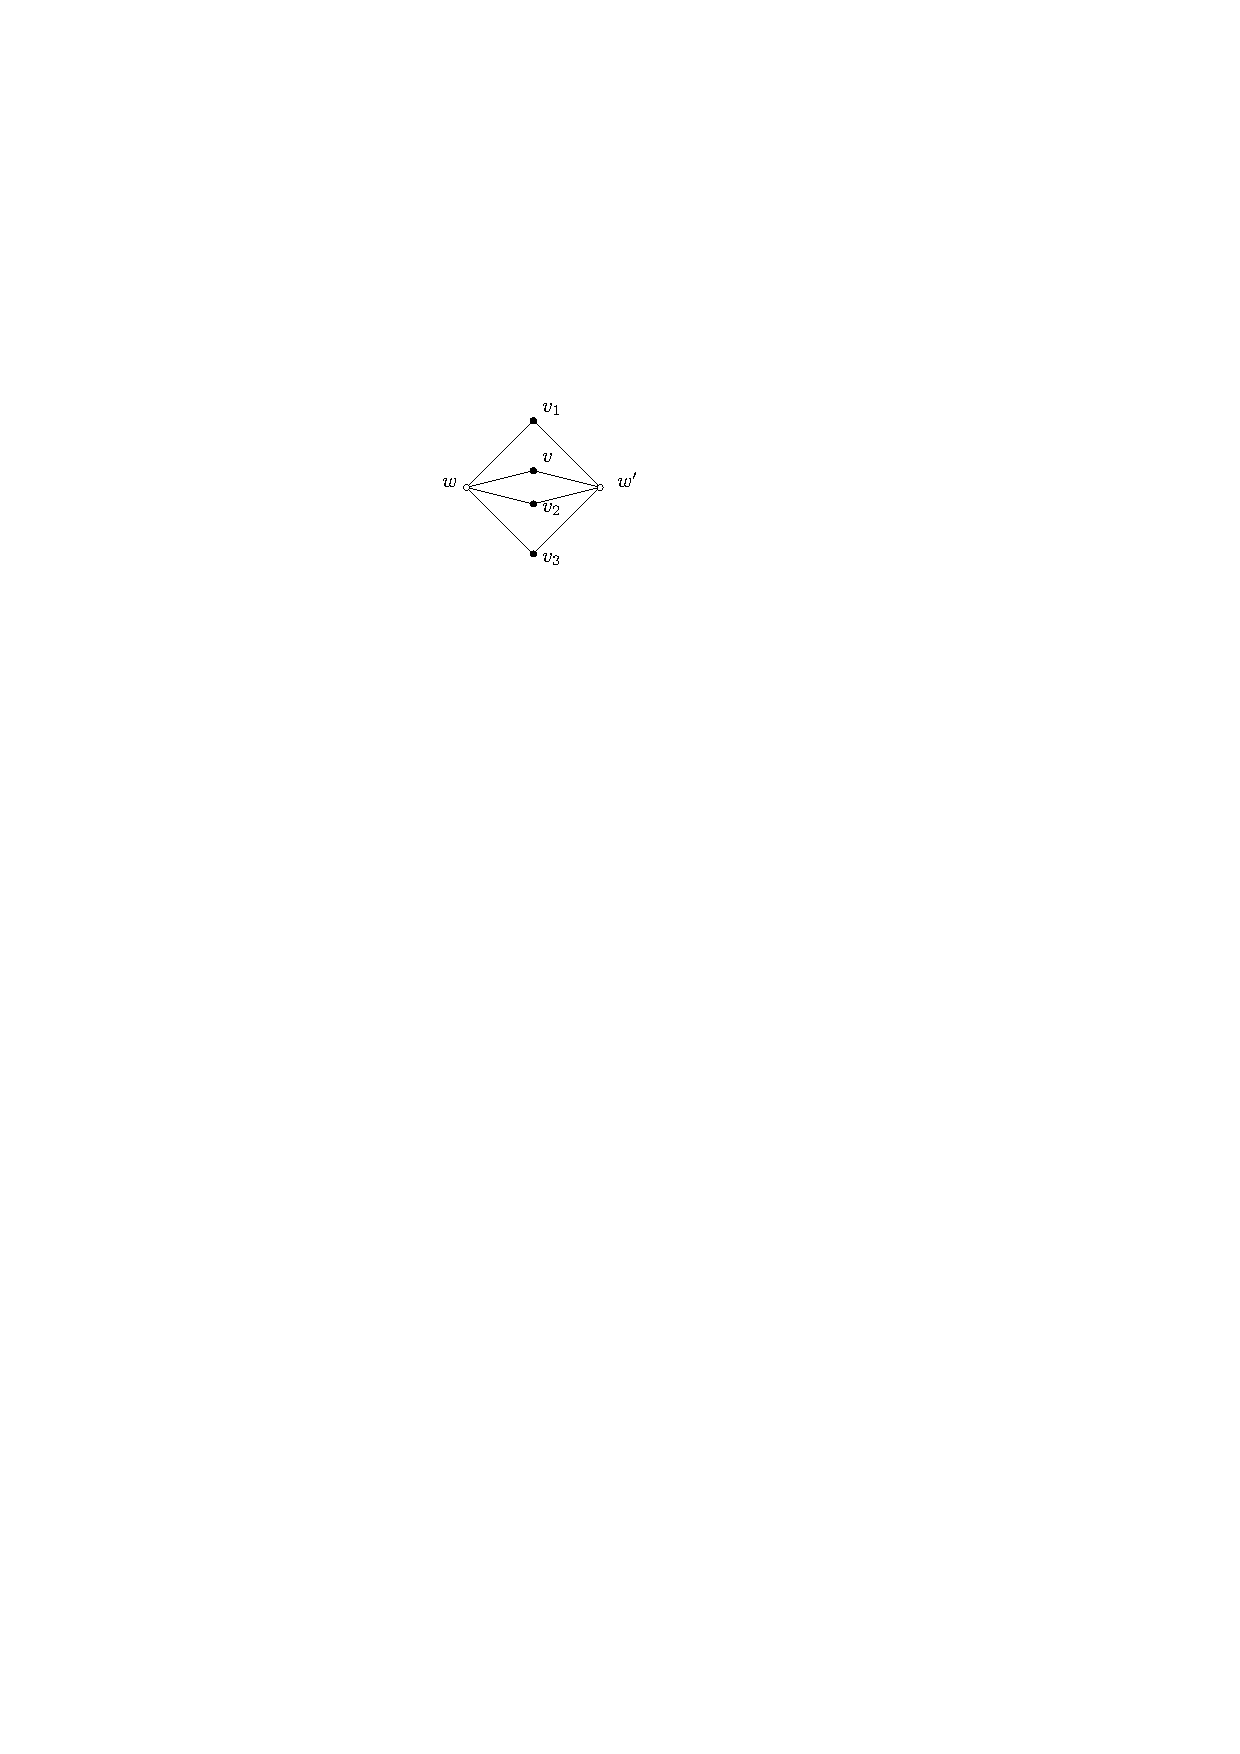
\includegraphics[width=0.25\textwidth]{Figures/series-reduction1.pdf}} \qquad
\fbox{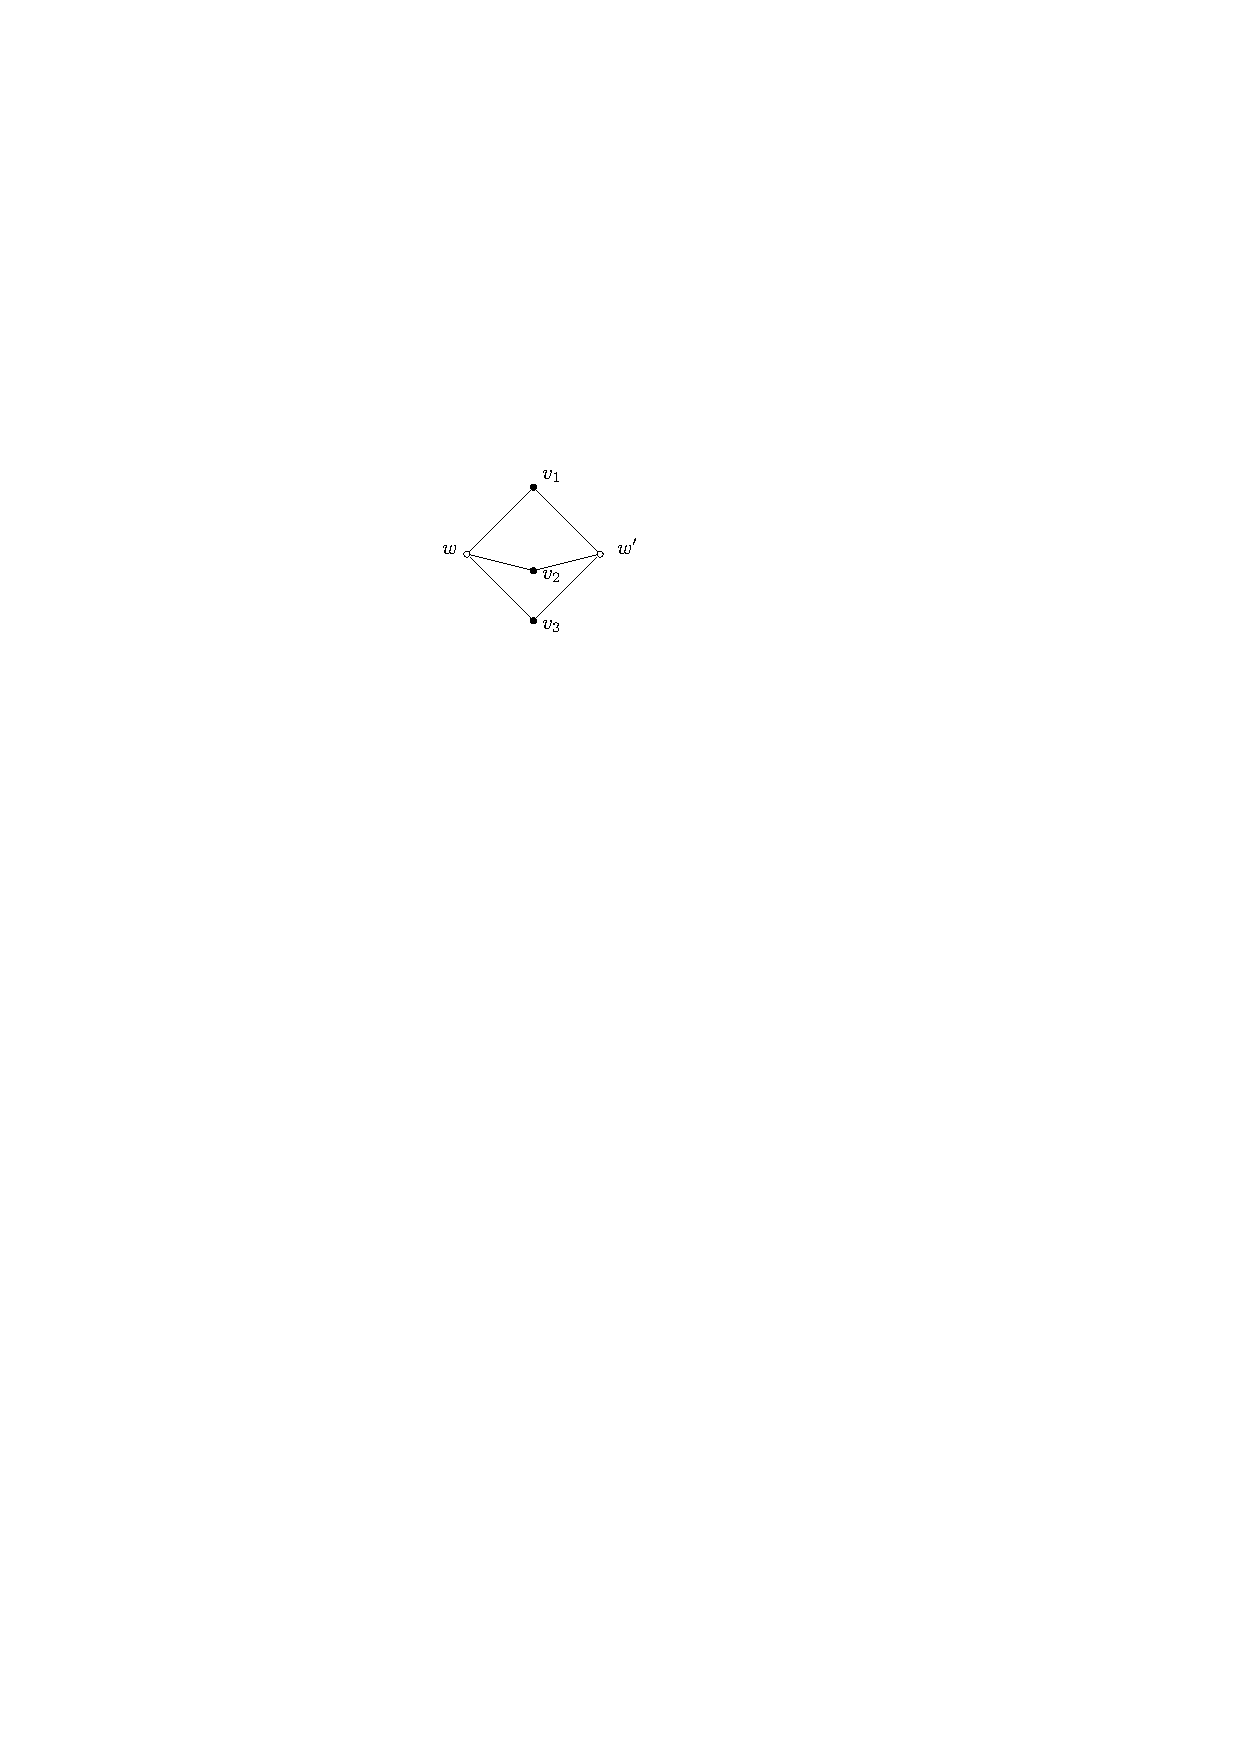
\includegraphics[width=0.25\textwidth]{Figures/series-reduction2.pdf}} \qquad
\fbox{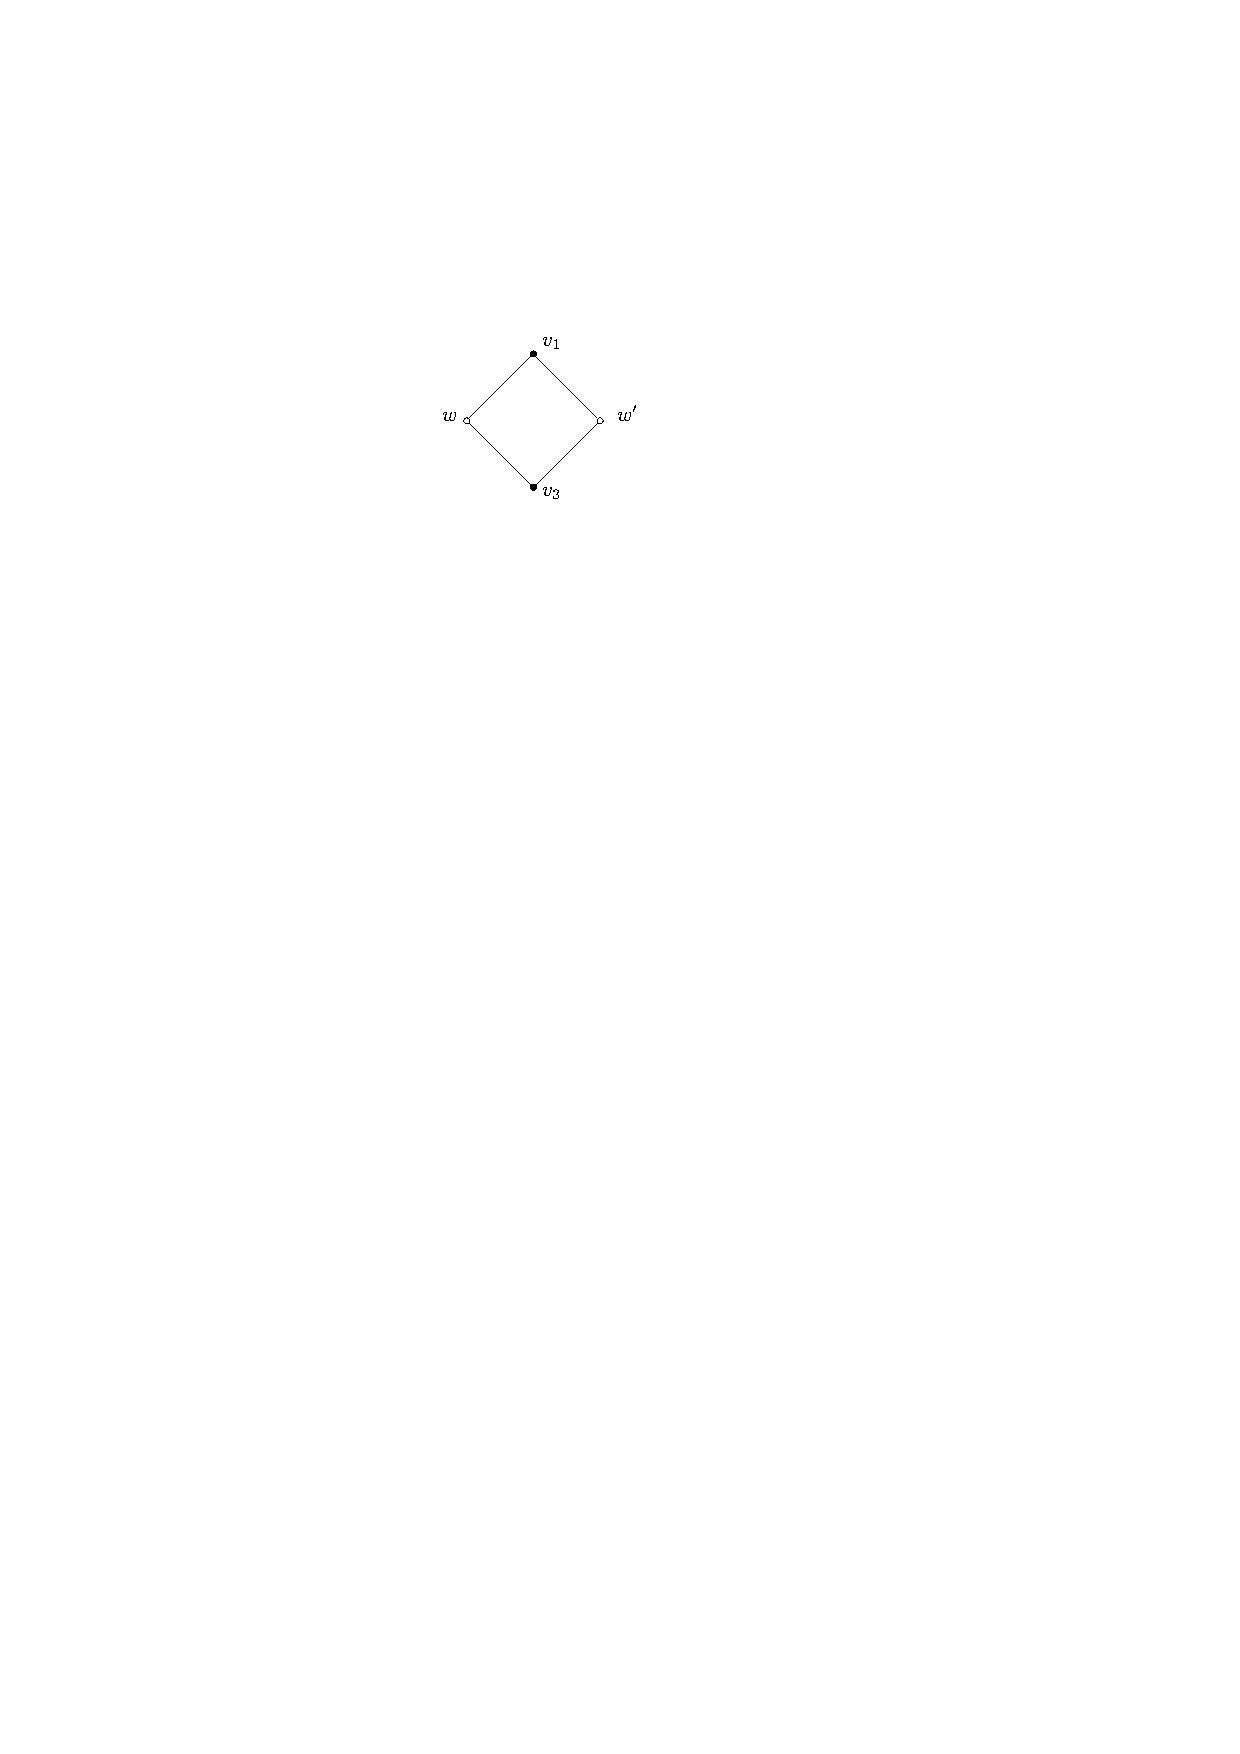
\includegraphics[width=0.25\textwidth]{Figures/series-reduction3.pdf}}
\caption{Series reduction of an orthodiagonal map; from left to right the vertices~$v$ and~$v_2$ in~$\V^{\bullet}$ of degree two are removed. The same labeling scheme as Figure~\ref{fig:orthogonal-diagonal} is used.}
\label{fig:series-reduction}
\end{figure}

\begin{figure}
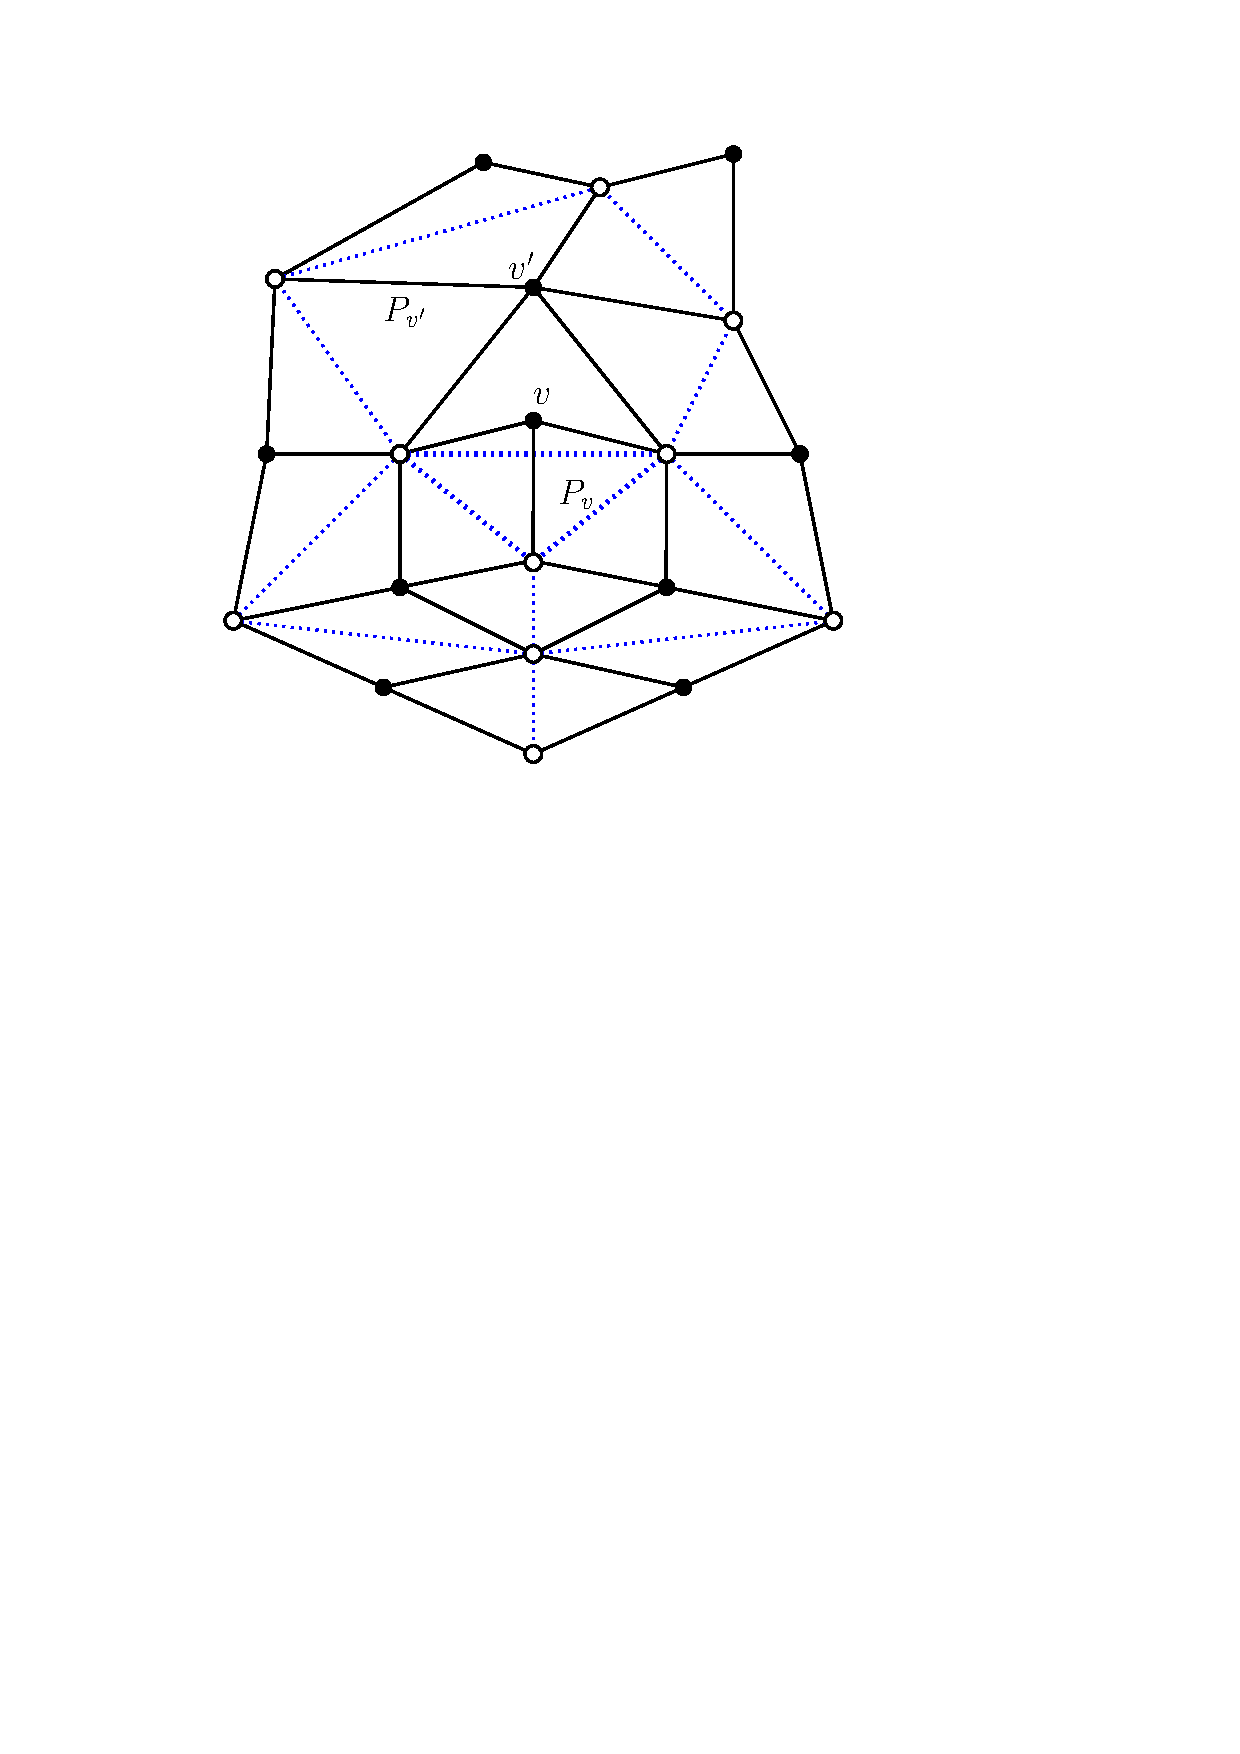
\includegraphics[width=0.35\textwidth]{Figures/orthomap-nonconvexPv.pdf}
\caption{A vertex~$v$ in an orthodiagonal map which is not contained in its corresponding polytope~$P_v$
but contained in a polytope of a neighbor~$P_{v'}$. The same labeling scheme as Figure~\ref{fig:orthogonal-diagonal} is used.}
\label{fig:concave-complication}
\end{figure}

\begin{remark}
\label{remark:orthodiagonalmaps}
Recall the definition of orthodiagonal map from Section~\ref{subsection:orthodiagonal}. In the case some quadrilaterals in~$\G$ are nonconvex, the construction there may fail 
to produce an orthogonal tiling. In this remark, we explain how our proof still applies to this case.

We first observe that we can use electric network laws to reduce to the case where all interior vertices in~$\G^{\bullet}$ and~$\G^{\circ}$ have degree at least three. An interior vertex in~$\G$ must be incident to at least two inner faces, so every interior vertex in~$\G^{\bullet}$ has degree at least two. An interior vertex~$v$ in~$\G^{\bullet}$ with exactly two neighbors~$v_1, v_2 \in \G^{\bullet}$ must share an edge in~$\E$ with exactly two vertices~$w, w' \in \V^{\circ}$. Thus, by the series law, any function~$f: \V^{\bullet} \to \R$ which is~$\mathbf{a}$-discrete harmonic must also be~$\mathbf{a}$-discrete harmonic on the graph where the vertex~$v$ and its two incident edges in~$\G$ is removed --- see Figure~\ref{fig:series-reduction}. Indeed, since~$v_1$ and~$v_2$ are neighbors of~$v$ and~$w-w'$ is orthogonal to~$v-v_1$ and~$v - v_2$, the vertex~$v$ lies on the line segment between~$v_1$ and~$v_2$; therefore
\[
\frac{\|v_1 - v_2\|}{\|w - w'\|} = \frac{\|v_1 - v\| + \|v - v_2\|}{\|w - w'\|}  = \frac{1}{\mathbf{a}(v_1, v)} + \frac{1}{\mathbf{a}(v_2, v)} \, . 
\]
Similarly, by the parallel law, we may reduce to the case there are no internal vertices in~$V^{\circ}$ of degree less than three. 
The result of Theorem~\ref{theorem:2d} on the reduced graph implies the result on the non-reduced graph. Indeed, arguing with the maximum principle for discrete harmonic functions and the mean-value property as in the proof of Theorem~\ref{theorem:2d}, if a discrete harmonic function is close to a continuum harmonic function on the reduced graph, then it must be close to the same continuum harmonic function on the deleted vertices.

Every vertex~$v \in \V^{\bullet}$ is now associated to a well-defined strictly convex polygon~$P_v$ with edges given by the opposite diagonals of the quadrilaterals
containing~$v$. The polygons~$\{P_v\}_{v \in \V^{\bullet}}$ have pairwise disjoint interiors. Every vertex~$v \in \V^{\bullet}$ 
is either contained in the interior of~$P_v$ or in the interior of~$P_{v'}$ where~$v' \in \V^{\bullet}$ is a neighbor of~$v$ --- see Figure~\ref{fig:concave-complication}.

We also define, for each edge~$e = (v,v') \in \mathcal{E}^{\bullet}$, the set~$Q_e$ to be the quadrilateral in~$\G$ with extremal vertices~$v$ and~$v'$. Note for convex quadrilaterals, this coincides with~$\Qe$ defined in~\eqref{eq:qeset}. 

With these two modified definitions, the proof of Theorem~\ref{theorem:2d} proceeds in the exact same way. 
\end{remark}



\subsection{All dimensions with smallness hypotheses}
% CLOSE 4: The iteration uses the internal-source energy bound, not the full-error column proposition.
We now iterate the internal-source energy bound~\eqref{eq:internal-energy} and the full-projection inequality from Lemma~\ref{lemma:ptype-inequality}, together with an assumption on tiny polytopes, to obtain a pointwise bound. The following bound on the measure of dual polytopes corresponding to edges with large gradient motivates the weighted estimate in the iteration.


\begin{lemma}[Weighted gradient-energy estimate]
	\label{lemma:gradient-energy-estimate}
	For every bounded set of vertices~$A$ with~$\overline A \subset \V$ and function~$f: \overline{A} \to \R$  we have
	the bound
	\[
	 \sum_{e \in \E[\overline{A}]} d \vol_{d}(\Qe)  1\{ |\nabla^{\mathcal{G}} f(e)| > \delta\}  \leq \D(f, A) 	 \qquad \forall \delta \geq \sup_{e \in \E[\overline{A}]} \|e\| \, . 
	\]
\end{lemma}
\begin{proof}
	We compute, using the assumption~$\delta \geq \sup_{e \in \E[\overline{A}]} \|e\|$, 
	\begin{align*}
		\D(f, A)  =  \sum_{e \in \E[\overline{A}]} \frac{\vol_{d-1}(H_e)}{\|e\|} |\nabla^{\mathcal{G}} f(e)|^2  
		&\geq \sum_{e \in \E[\overline{A}]} \frac{\vol_{d-1}(H_e)|}{\|e\|} \delta^2 1\{ |\nabla^{\mathcal{G}} f(e)| > \delta\} \\
		&\geq \sum_{e \in \E[\overline{A}]} \vol_{d-1}(H_e) \|e\|   1\{ |\nabla^{\mathcal{G}} f(e)| > \delta\}  \\
		&= \sum_{e \in \E[\overline{A}]} d \vol_{d}(\Qe)  1\{ |\nabla^{\mathcal{G}} f(e)| > \delta\}  \, , 
	\end{align*}
	where in the last step we used Lemma~\ref{lemma:geometry-bound}. 
\end{proof}

\begin{theorem}
		\label{theorem:generaldim}
	Let~$U$ be a bounded domain with~$\overline{U} \subset \mathcal{D} \subset \R^d$ and suppose~$h_C \in C^{2}(\GCU)$ satisfies~$\CLap h_C = 0$ on~$\GCU$ and let~$h_D: \overline{\V[U]} \to \R$ satisfy 
	\[
	\left\{
	\begin{aligned}
		&  \aDelta h_D = 0 & \mbox{in} & \ \V[U] \,,
		\\
		& h_D = h_C & \mbox{on} & \  \partial \V[U] \, . 
	\end{aligned}
	\right.
	\]
	Then, there exists~$C= C(U) < \infty$ such that, with
	\[
% CLOSE 4: Retain the higher-dimensional bound with the internal Taylor constant only.
	\eps := \sup_{v \in \overline{\V[U]}} \diam(P_v) \quad L := \sup_{\GCU} |\Cnabla h_C| \quad \mbox{and} \quad M := M_U^\circ(h_C) \vee 1 \, , 
	\]
	and for any fixed~$K \geq 1$, which can depend on~$\eps$,
	\begin{equation}
		\begin{aligned}
		\label{eq:small-volume-assumption}
		\mathcal{A} := \{ v \in \overline{\V[U]} : \vol_{d}(P_v) < \eps^{K}  \}  \quad \mbox{and} \quad
		D := \sup_{\mbox{components $Q \subset \mathcal{A}$}} {\sum_{v \in Q} \diam(P_v)}  \, , 
		\end{aligned}
	\end{equation}
	where the supremum is over the connected components of the subgraph induced by~$\mathcal{A}$, we have, assuming~{$\eps  < (C M)^{-1}$},
	\begin{equation} 
		\label{eq:full-bound}
{	 \sup_{v \in \V[U]} | h_D(v) - h_C(v) | \leq C M K \eps(\log \eps^{-1}) + D L  \, .}
	\end{equation}
\end{theorem}


	Note that if for some large~$K$ the set~$\mathcal{A}$ in~\eqref{eq:small-volume-assumption} is empty, then the second error term 
	in~\eqref{eq:full-bound} is zero. 
% CORRECTION 11: A flux supported on internal edges removes the boundary-cell gap in the iteration.
% CLOSE 4: Use the cell-only boundary estimate and account for original boundary edges in the terminal comparison.
\begin{proof}[Proof of Theorem~\ref{theorem:generaldim}]
We give an iteration which will also prove Theorem~\ref{theorem:generaldim-decay}. If $A:=\V[U]$ is empty there is nothing to prove. Retain $m(S)$, $g_S$, $M_0$, and the estimates~\eqref{eq:internal-flux}--\eqref{eq:initial-boundary-correction} from the internal-edge comparison preceding Theorem~\ref{theorem:2d}. All zero-boundary functions are extended by zero to $\overline A$.
Choose $R_0$ with $U\subset B_{R_0}$ and assume $\eps\le1/2$. All cells under consideration lie in $B_{R_0+2}$; put $H=2(R_0+2)$ and $B=d\vol_d(B_{R_0+2})$. Their Euclidean diameter and coordinate spans are at most $H$, and $m(A)\le B$.

Set $S_0=A$. Given $S_i$, choose $0<\delta_i\leq\eps$ bounding its cell diameters, put $g_i=g_{S_i}$, and define
\begin{align*}
 N_{i+1}&=\{v\in S_i:|g_i(v)|>aM\delta_i\},\\
 S_{i+1}&=\{v\in N_{i+1}:|g_i(v)-g_i(w)|>2\sqrt{\eps\delta_i}
                  \text{ for every }w\in\partial N_{i+1}\text{ adjacent to }v\}.
\end{align*}
If $S_i$ is empty, all subsequent sets and functions are empty or zero. Take $a\geq\max(1,24dH)$. The full-projection inequality in the proof of Lemma~\ref{lemma:ptype-inequality}, together with~\eqref{eq:internal-energy}, gives
\[
 \left|\bigcup_{v\in N_{i+1}}\projone(P_v)\right|\leq3a^{-1}m(S_i).
\]
The dual polytopes of edges with both endpoints in $N_{i+1}$ lie in the cylinder over this projection, of height at most $H$. An edge incident to $S_{i+1}$ not of this kind has $|\nabla^{\mathcal G}g_i(e)|>2\sqrt{\eps\delta_i}$. Since $\|e\|\leq2\eps$, Lemma~\ref{lemma:geometry-bound} gives
\[
 \sum_e d\vol_d(Q_e)1_{\{|\nabla^{\mathcal G}g_i(e)|>2\sqrt{\eps\delta_i}\}}
 \leq\frac{\eps}{\delta_i}\D(g_i,S_i).
\]
Consequently, if $M\eps\leq1/12$,
\begin{equation}\label{eq:repaired-contraction}
 m(S_{i+1})\leq(3dH/a+9M^2\eps\delta_i)m(S_i)
               \leq\tfrac14m(S_i).
\end{equation}

Outside $S_{i+1}$ we have $|g_i|\leq aM\delta_i+2\sqrt{\eps\delta_i}$. On $S_{i+1}$ the difference $g_i-g_{i+1}$ has, in addition to these boundary values, a source supported on edges from $S_{i+1}$ to $S_i\setminus S_{i+1}$. Both endpoints of each such edge belong to $S_i$, so~\eqref{eq:internal-flux} and the boundary comparison give
\begin{equation}\label{eq:repaired-telescoping}
 \|g_i-g_{i+1}\|_\infty
 \leq aM\delta_i+2\sqrt{\eps\delta_i}+M_0\delta_i^2.
\end{equation}
This proves the iteration, including its boundary estimates.

For the present theorem use $\delta_i=\eps$. Choose
\[
 N=1+\max\left(0,\left\lceil\frac{\log B+K\log(\eps^{-1})}{\log4}\right\rceil\right).
\]
Then $4^{-N}m(A)<\eps^K$ and $N\le C(U,d)K\log(\eps^{-1})$: use $\lceil x\rceil\le x+1$ and $K\log(\eps^{-1})\ge\log2$ to absorb the fixed constants. Coverage by incident dual polytopes shows that every cell of $S_N$ has volume less than $\eps^K$. Thus each component $Q$ of $S_N$ is contained in a component of $\mathcal A$, and $D_Q:=\sum_{v\in Q}\diam(P_v)\le D$.

Let $f_Q$ be the harmonic extension of $h_C$ to $Q$, minus $h_C$. On $Q$, $g_N=g_Q$, so~\eqref{eq:cell-flux-bound} and boundary comparison give $\|g_N-f_Q\|_{Q,\infty}\le M_0\eps^2$.
For $v\in Q$ and $w\in\partial Q$, take a simple graph path in $Q$ to a neighbour of $w$ and append $w$. Join successive contact points within each convex cell, with endpoints $v,w$. Each cell of $Q$ is used at most once, so the path length is at most $D_Q+\eps$, including its last segment in $P_w$. Thus $|h_C(w)-h_C(v)|\le L(D_Q+\eps)$, and the maximum principle gives the first bound below.
For the second, expand $\aDelta f_Q=-\aDelta h_C$ at each active endpoint. Edges into $A$ obey the finite Taylor inequality with $M$, and edges into $\partial A$ obey~\eqref{eq:broken-taylor-bound} with remainder at most $2M_0\eps^2$. With $q(x)=\|x-v\|^2$, comparison of $\pm f_Q+(M/2)q-2M_0\eps^2 1_Q$ therefore gives
\[
 |f_Q(v)|\leq\min\{L(D_Q+\eps),(M/2)\rho^2+2M_0\eps^2\},
 \qquad \rho=\max_{w\in\partial Q}\|w-v\|\leq\min(D_Q+\eps,H).
\]
If $L\le MH/2$, the first bound is at most $LD_Q+MH\eps/2$. If $L>MH/2$, use $\rho^2\le H(D_Q+\eps)$ in the second bound to obtain $LD_Q+MH\eps/2+2M_0\eps^2$. This accounts for the exit cell without changing the coefficient of $DL$.

Finally combine~\eqref{eq:initial-boundary-correction}, the first $N$ bounds~\eqref{eq:repaired-telescoping}, and this estimate for $g_N$. The sum is bounded by
\[
 DL+MH\eps/2+4M_0\eps^2+N(aM\eps+2\eps+M_0\eps^2).
\]
Since $M_0\le M$, $M\ge1$, and $\eps\le1/2$, the result is
$\|h_D-h_C\|_\infty\leq CMK\eps\log(\eps^{-1})+DL$.
Increase $C=C(U,d)$ to ensure the assumed smallness conditions. As in the published statement, the fixed ambient dimension is included in the dependence on $U$.
\end{proof}



We modify the previous proof to replace the assumption~\eqref{eq:small-volume-assumption} by one
where the diameter of every polytope is bounded by some (possibly tiny) power of the volume of its dual polytopes. 
\begin{theorem}
	\label{theorem:generaldim-decay}
	Let~$U$ be a bounded domain with~$\overline{U} \subset \mathcal{D} \subset \R^d$ and suppose~$h_C \in C^{2}(\GCU)$ satisfies~$\CLap h_C = 0$ on~$\GCU$ and let~$h_D: \overline{\V[U]} \to \R$ satisfy 
	\[
	\left\{
	\begin{aligned}
		&  \aDelta h_D = 0 & \mbox{in} & \ \V[U] \,,
		\\
		& h_D = h_C & \mbox{on} & \  \partial \V[U] \, . 
	\end{aligned}
	\right.
	\]
	Then with
	\[
% CLOSE 4: Use only internal-edge Taylor remainders in the decay theorem as well.
	\eps := \sup_{v \in \overline{\V[U]}} \diam(P_v) \quad \quad M := M_U^\circ(h_C) \vee 1 \, , 
	\]
	and under the assumption that there exists some~$F, \alpha > 0$ such that
	\begin{equation}
		\label{eq:decay-of-stuff}
		\diam(P_v) \leq  F \sup_{e = (w,v) \in \E} \vol_{d}(\Qe)^{\alpha} \qquad \forall v \in \V[U] \, ,  
	\end{equation}
	we have that there exists~$C=C(U, F, \alpha) < \infty$ such that, assuming~{$\eps  < (C M)^{-1}$},
	\begin{equation} 
		\label{eq:full-bound-decay-of-stuff}
		\sup_{v \in \V[U]} | h_D(v) - h_C(v) | \leq {C M \eps (\log \eps^{-1})}  \, . 
	\end{equation}
\end{theorem}
% CORRECTION 11: Use the boundary-corrected iteration for the decay hypothesis.
% CLOSE 5: Correct the geometric-decay product and use the cell-only boundary costs.
\begin{proof}
If $A=\V[U]$ is empty there is nothing to prove. Otherwise use the internal-edge comparison and the iteration in the preceding proof, with
$\delta_i=\max_{v\in S_i}\diam(P_v)$ for nonempty $S_i$. By~\eqref{eq:repaired-contraction}, $m(S_i)\leq4^{-i}m(A)$. Every edge incident to a vertex of $S_i$, including every boundary edge, occurs in $m(S_i)$. Thus~\eqref{eq:decay-of-stuff} gives
\[
 \delta_i\leq\min\{\eps,C_0 4^{-\alpha i}\},
 \qquad C_0=F(m(A)/d)^\alpha.
\]
In particular the sets eventually become empty: otherwise a fixed finite collection of cells of positive diameter would have diameters tending to zero.

For completeness choose $J=\max(0,\lceil\log(C_0/\eps)/(\alpha\log4)\rceil)$, taking $J=0$ if $A$ is empty. For $i<J$ both $\delta_i$ and $\sqrt{\eps\delta_i}$ are at most $\eps$. For $i=J+j$ they are bounded, respectively, by $\eps4^{-\alpha j}$ and $\eps4^{-\alpha j/2}$. Therefore
\[
 \sum_i\delta_i\leq\eps\left(J+\frac1{1-4^{-\alpha}}\right),\qquad
 \sum_i\sqrt{\eps\delta_i}\leq\eps\left(J+\frac1{1-4^{-\alpha/2}}\right).
\]
The bound on $m(A)$ in the preceding proof implies $J+1\leq C(U,F,\alpha)\log(\eps^{-1})$ for $\eps\leq1/2$. Also $\sum_i\delta_i^2\leq\eps\sum_i\delta_i$.
Telescoping until the selected set is empty and using~\eqref{eq:initial-boundary-correction} proves
\[
 \|h_D-h_C\|_\infty
 \leq M_0\eps^2+\sum_i(aM\delta_i+2\sqrt{\eps\delta_i}+M_0\delta_i^2)
 \leq CM\eps\log(\eps^{-1}).
\]
Taking $C$ large enough guarantees $M\eps\leq1/12$ and $\eps\leq1/2$. No bound on the diameters of exterior boundary cells by $\delta_i$ has been used.
\end{proof}



% CORRECTION 12: Use a fixed harmonic neighbourhood and K at least one.
% CLOSE 6: A fixed harmonic neighbourhood uniformly bounds the smaller internal Taylor constant.
\begin{proof}[Proof of Theorem~\ref{theorem:convergence-of-the-dirichlet-problem} under Hypothesis~\ref{item:cont-neighborhood}]
Choose a fixed compact neighbourhood of $\overline U$ in $\intr\mathcal D$ on which $h_C$ is harmonic. For all sufficiently large $n$, it contains $K_U$: every cell in $\widehat U$ is within $2\eps_n$ of $U$, and an incident edge segment is also within $2\eps_n$ of its endpoint in $U$. Taylor's integral formula on the internal segments bounds $M_U^\circ(h_C)$ by the fixed neighbourhood Hessian supremum. Thus all constants required above are uniform, and the active cells are complete. The same reasoning applies to every finite active set in a fixed collar, including the ball sets used to deduce Theorem A; it does not add a hypothesis to that theorem or to Theorem B(b).
The assertions under~\ref{item:planarity} and~\ref{item:diam} follow from Theorems~\ref{theorem:2d} and~\ref{theorem:generaldim-decay}, using Lemma~\ref{lemma:geometry-bound} to convert the latter hypothesis. Under~\ref{item:vol}, write $v_n=\inf_{v\in\V_n}\vol_d(P_v)$ and choose
\[
 K_n=1+\frac{\max(0,\log(v_n^{-1}))}{\log(\eps_n^{-1})}\geq1.
\]
For $\eps_n<1$, we have $\eps_n^{K_n}<v_n$, so $\mathcal A$ is empty. Moreover
$K_n\eps_n\log(\eps_n^{-1})
=\eps_n\log(\eps_n^{-1})+\eps_n\max(0,\log(v_n^{-1}))\to0$.
Theorem~\ref{theorem:generaldim} proves the conclusion.
\end{proof}







\section{Convergence of random walk modulo time paramaterization} 
\label{sec:rw-convergence}
In this section we prove a ``black box theorem'' which roughly states that if you have convergence of the Dirichlet 
problem, then the trace of random walk converges, under rescaling, to the trace of Brownian motion. Slightly more precisely,  we show that under this condition, the law of the rescaled random walk converges to the law of Brownian motion with respect to the local topology on curves viewed modulo time parameterization. 

Specifically, we fix a sequence of undirected graphs~$\{\G_n = (\V_n, \E_n)\}_{n\geq0}$
with each~$\V_n \subset \Rd$.  For a point~$z \in \Rd$, let~$z^{n}$ be the nearest vertex in~$\G_n$, with ties broken in lexicographical ordering.  
We also fix a nearest neighbor discrete-time random walk~$\{X_t^{n}\}_{t \geq 0}$ on~$\V_n$; that is,~$\{X_t^{n}\}$ is a time homogeneous Markov chain and~$(X_{t}^{n}, X_{t+1}^{n}) \in \E_n$ for all~$t \geq 0$. We let~$\Delta^{\G_n}$ denote the generator of~$X_t^{n}$, that is,
for every vertex~$a \in \V_n$ and function~$f: \V_n \to \R$, 
\[
\Delta^{\G_n} f(a) = \mathbb{E}[f(X^{a, n}_1) - f(a)] \, , 
\]
where the expected value is taken over one step of the random walk with initial point~$a \in \V_n$. 



 We define, for a set~$U \subset \Rd$ and~$r > 0$, 
\[
B_{r}(U) := \{ x \in \Rd : \inf_{y \in U}\| x - y\| \leq r\} \, . 
\]
 The following assumption states that the graph approximates some (possibly infinite) domain~$\mathcal{D}$ and the Dirichlet problem for every ball~$B_r(x)$ intersecting a neighborhood of~$\mathcal{D}$ converges. 
 
% CORRECTION 13: Specify the test-data and solution quantifiers in Assumption D.
In this section a harmonic test function is given values on $\Rd$, with harmonicity required only on the indicated neighbourhood. Thus its boundary values are defined even at distant exit vertices. In~\eqref{eq:convergence-of-d-problem} convergence is required for every choice of solutions as $n$ varies. The proofs use only bounded continuous global test functions. These conventions make explicit the meaning of the Dirichlet extensions in the assumption.
\begin{assumptionD}
	\label{ass:D}
	{There exists a domain~$\mathcal{D}$ and some~$\delta > 0$ such that for every~$r > 0$ and~$x \in B_{\delta}(\mathcal{D})$ the following holds for~$B := B_r(x) \cap B_{\delta}(\mathcal{D})$.} The graph approximates Euclidean space in the ball, 
	\begin{equation}
		\label{eq:local-approximation-of-space}
	\lim_{n \to \infty} \sup_{z \in B} \| z^{n} - z\| = 0 \, . 
	\end{equation}
	Moreover, for every function~$h_C$ which is continuum harmonic in a neighborhood of~$B$, the discrete
	harmonic extension~$h^{n}_D$ of~$h_C$ to~$\V_n[B]$, defined by, 
	\[
	\left\{
	\begin{aligned}
		&  \Delta^{\G_n} h^{n}_D = 0 & \mbox{in} & \ \V_n[B] \,,
		\\
		& h^{n}_D = h_C & \mbox{on} &  \ \partial \V_n[B]    \, ,
	\end{aligned}
	\right.
	\]
	converges uniformly to~$h_C$,
	\begin{equation}
		\label{eq:convergence-of-d-problem}
	\lim_{n \to \infty} \sup_{z \in \V_n[B]} |h^{n}_D(z) - h_C(z)|  = 0 \, . 
	\end{equation}
\end{assumptionD}

%We first record by Theorems~\ref{theorem:2d},~\ref{theorem:generaldim}, and~\ref{theorem:generaldim-decay}, that 
%\begin{lemma}
%	\label{lemma:ass-satisfied}
%	Assumption~\ref{ass:D} is satisfied for the graphs in Theorem~\ref{theorem:convergence-of-rw-trace}.  
%\end{lemma}
%\begin{proof}
%	The convergence~\ref{eq:convergence-of-d-problem} follows immediately from Theorems~\ref{theorem:2d},~\ref{theorem:generaldim}, and~\ref{theorem:generaldim-decay}. 
%	To see~\eqref{eq:local-approximation-of-space} we let~$z \in B$ be given and observe that 
%	since the tiles of~$\G$ are uniformly bounded, there will be, for all~$\eps$ sufficiently small, 
%	a vertex~$v \in \V$ a bounded distance away from~$\eps^{-1} z$. 
%\end{proof}





Under this assumption, we prove a central limit theorem.

\begin{theorem}
	\label{theorem:general-clt}
	Suppose~$\mathcal{D}$ is such that Assumption~\ref{ass:D} holds and let~$U \subset \mathcal{D}$ be a {Lipschitz}, bounded domain. Let~$z \in U$, and let~$X^{z, n}$ be random walk on~$\G_n$ 
	started at~$z^{n}$, let~$J^{z, n}_U$ denote the first exit from~$\V_n[U]$,
	and let~$Y^{z, n}$ denote the piecewise linear interpolation of~$X^{z, n}$.
	Let~$\mathcal{B}^z$ be a standard Brownian motion started at~$z \in U$ with first exit~$\tau^{z}_U$ from~$U$. 
	The supremum over all~$z \in U$ of the Prokhorov distance between the laws of~$Y^{z, n} \vert_{[0,J^{z, n}_U]}$ and~$\mathcal{B}^{z} \vert_{[0, \tau^{z}_U]}$ with respect to the metric~\eqref{eq:cmp-topology} converges to 0 as~$n \to \infty$. 
\end{theorem}

% CORRECTION 12: Apply the ball argument in a collar of U; project boundary data in part (b).
\begin{proof}[Proof of Theorem~\ref{theorem:convergence-of-rw-trace} assuming Theorem~\ref{theorem:general-clt}]
Choose $\rho>0$ so that $B_{3\rho}(U)\subset\intr\mathcal D$, and use the auxiliary domain $D_0=\{x:\dist(x,U)<\rho\}$ in Assumption~\ref{ass:D}, with $\delta=\rho$. Every set $B_r(x)\cap B_\rho(D_0)$ is contained in the fixed collar $B_{2\rho}(U)$. The estimates of Section~\ref{sec:iteration} and the proof of Theorem B(a) apply to its finite active vertex set, irrespective of whether that set is connected or its Euclidean union is a domain. A function harmonic near this compact set has uniform derivative bounds on its cell and segment support for large $n$. Thus Theorem B(a), in this finite-set form, proves~\eqref{eq:convergence-of-d-problem}. The approximation~\eqref{eq:local-approximation-of-space} follows from~\eqref{eq:smallness}. Theorem~\ref{theorem:general-clt} applied with $D_0$ proves the assertion, including uniformity in $z$.
\end{proof}

\begin{proof}[Proof of Theorem~\ref{theorem:convergence-of-the-dirichlet-problem} assuming Hypothesis~\ref{item:hypb}]
For all large $n$ the active cells are complete and the finite Dirichlet solution is unique. Its value at $v\in\V_n[U]$ is
$\mathbb E_v h_C(\pi_U(X_T))$ by the stopped martingale argument. Every exit vertex has distance at most $2\eps_n$ from $\overline U$, since it is adjacent to a vertex in $U$; hence $\|\pi_U(X_T)-X_T\|\leq2\eps_n$.

The bounded harmonic function $h_C$ also satisfies
$h_C(v)=\mathbb E_v h_C(\mathcal B_{\tau_U})$: stop its harmonic martingale on an increasing compact exhaustion of $U$, and use bounded convergence, continuity on $\overline U$, and almost sure finite exit from a containing ball. Approximate $h_C$ uniformly on $\overline U$ by bounded Lipschitz functions on $\Rd$. Explicitly, clip
$f_L(x)=\inf_{y\in\overline U}(h_C(y)+L\|x-y\|)$
to the range of $h_C$; uniform continuity shows that $f_L\to h_C$ uniformly on $\overline U$ as $L\to\infty$. For each fixed $L$, Theorem A and continuity of the endpoint map give convergence of the exit expectations of $f_L$, uniformly in the start. The projection changes the discrete expectation by at most $2L\eps_n$. Let $n\to\infty$ and then $L\to\infty$. This proves~\eqref{eq:convergence-of-d-general} uniformly in $v$.
\end{proof}



It remains to prove Theorem~\ref{theorem:general-clt}. We first show that Assumption~\ref{ass:D} implies convergence of harmonic measure. We then use the strong Markov property  of random walk together with an approximation argument to deduce Theorem~\ref{theorem:general-clt}. 




\subsection{Convergence of harmonic measure}
% CORRECTION 13: Use the same ball convention in the notation and proposition.
Let~$\B$ denote an open ball in~$\Rd$.
Let~$\hm(x)$ be the harmonic measure on~$\partial \B$, as seen from~$x \in \B$. For~$x \in \B$ and~$z \in \partial \V_n[\B]$, we define~$\hmn(x)[z]$ to be the probability measure which assigns 
mass to each vertex of $\partial\V_n[\B]$ equal to its discrete harmonic measure from $x^n$. We also write~$\dPr$ for the Prokohorov distance between two probability measures. 
 
 
% CORRECTION 13: Localize the harmonic-measure statement and prove it without a step-size assumption.
\begin{prop} \label{prop:convergence-of-harmonic-measure}
Under Assumption~\ref{ass:D}, let $\B$ be any open ball with $\overline\B\subset B_\delta(\mathcal D)$. Then
\[
 \lim_{n\to\infty}\sup_{x\in\B}\dPr(\hmn(x),\hm(x))=0.
\]
For all sufficiently large $n$ the walk exits $\V_n[\B]$ almost surely, so the discrete measures in this formula are probability measures.
\end{prop}
\begin{proof}
We make explicit the usual quantifiers in Assumption~\ref{ass:D}: convergence is required for every choice of solutions, and a test function harmonic near $B$ is given bounded values on the remaining vertices before its Dirichlet problem is formed. One may take any bounded continuous extension to $\Rd$; the arguments use functions with such extensions. This also resolves evaluation at exit vertices outside the neighbourhood where harmonicity is required.

First the assumption for $h_C=0$ forces almost sure exit for all large $n$. Indeed the survival probability $s_n(v)=\P_v[T=\infty]$ is a bounded harmonic function on the active vertices, zero on the boundary, by the Markov property. If $\sup s_n>0$ for infinitely many $n$, choose the zero-data solution $s_n/\sup s_n$ at those indices, and zero at the others. Its supremum equals one infinitely often, contradicting~\eqref{eq:convergence-of-d-problem}. Thus $s_n=0$ eventually. Bounded boundary data then have the unique bounded extension given by their exit expectation: stop the bounded harmonic martingale at $T\wedge k$ and use bounded convergence. If a nearest vertex $x^n$ is already outside the ball, its exit time is zero and its exit position is $x^n$.

Write $\B=B_R(c)$ and $a_n=\sup_{x\in\overline\B}\|x^n-x\|\to0$. For $\eta>0$ choose a bounded continuous cutoff equal to one on a neighbourhood of $\overline\B$ and zero outside $B_{R+\eta}(c)$, with values in $[0,1]$. It is harmonic near $\overline\B$. Applying the assumption and the exit-expectation representation shows, uniformly in $x\in\B$, that
\begin{equation}\label{eq:exit-annulus}
 \P_{x^n}[\|X_T-c\|>R+\eta]\longrightarrow0.
\end{equation}
An exit vertex is outside $\B$, and a starting vertex outside $\B$ is at most $a_n$ from its boundary. Thus exit positions concentrate uniformly near the sphere. This conclusion does not assume a bound on all graph edges.

Fix a bounded continuous function $f$ on $\Rd$ and an error $b>0$. Let $h_\kappa$ be the Poisson extension of the data $f$ from $\partial B_{R+\kappa}(c)$ to that larger ball. As $\kappa\downarrow0$, its values on $\partial\B$ converge uniformly to $f$. For example, for Lipschitz $f$ this follows from
$\mathbb E_s\|\mathcal B_{\tau_{R+\kappa}}-s\|^2=(R+\kappa)^2-R^2$ for $s\in\partial\B$, by stopping the coordinate and squared-norm martingales; continuous $f$ follows by uniform approximation on a compact ball. Choose $\kappa$ so that this error is below $b$. The continuum maximum principle gives $|h_\kappa-h_f|\leq b$ on $\overline\B$, where $h_f$ is the Poisson extension from $\partial\B$.

Extend $h_\kappa$ boundedly and continuously to $\Rd$, retaining it on a smaller neighbourhood of $\overline\B$. By continuity choose $\eta>0$ so that $|h_\kappa-f|\leq2b$ on the annulus $R\leq\|z-c\|\leq R+\eta$. Assumption~\ref{ass:D}, uniform continuity at the starting point, and~\eqref{eq:exit-annulus} now yield
\[
 \limsup_n\sup_{x\in\B}
 \left|\mathbb E_{x^n}f(X_T)-\mathbb E_x f(\mathcal B_{\tau_\B})\right|\leq3b.
\]
Let $b\downarrow0$.

To pass from individual tests to Prokhorov distance uniformly in the starting point, use~\eqref{eq:exit-annulus} to restrict both exit laws to one fixed compact ball, at an arbitrarily small error. The functions bounded by one and with Lipschitz constant at most one have finite uniform nets on that compact set: specify their values to fixed accuracy on a finite spatial net and use the Lipschitz inequality between net points. Apply the preceding convergence to this finite collection of tests. The resulting bounded Lipschitz distance tends to zero uniformly. If that distance is at most $b^2$, testing with $b(1-\dist(\cdot,F)/b)_+$ for any closed set $F$ gives $\mu(F)\leq\nu(F^b)+b$, and the reverse inequality likewise. This is precisely the Prokhorov bound $\dPr(\mu,\nu)\leq b$.
\end{proof}

The proposition applies to all translated and rescaled balls with closure in the stated neighbourhood.





\subsection{Convergence of random walk}
The argument given here is similar to the proofs of~\cite[Lemma 3.14 and Theorem 3.10]{GMSInvariance}.


% CORRECTION 14: Complete the finite-ball coupling and the stopping-at-the-boundary argument.
\begin{proof}[Proof of Theorem~\ref{theorem:general-clt}]
Only the convergence of ball-exit laws in Proposition~\ref{prop:convergence-of-harmonic-measure} will be used. We give the details needed for uniformity and for stopping at $\partial U$.

Fix $\eta>0$ so small that $B_{10\eta}(U)\subset B_\delta(\mathcal D)$. Take as centres $c_j$ the grid points of spacing $\eta/(10\sqrt d)$ in $B_{5\eta}(U)$. Their inner quarter-balls cover $B_{4\eta}(U)$, by coordinate rounding. Choose continuous weights $p_j(x)\geq0$, summing to one on $B_{4\eta}(U)$, with $p_j(x)=0$ unless $\|x-c_j\|<\eta/4$, by normalizing the functions $(\eta/4-\|x-c_j\|)_+$. All balls $B_\eta(c_j)$ have closure in $B_\delta(\mathcal D)$.

At each stage, from the current position $x$, choose $j$ with probabilities $p_j(x)$ and run the process until its first exit from $B_\eta(c_j)$. Do this for Brownian motion and for the walk, using their respective current positions. For Brownian motion choose $a\in(2\eta,3\eta)$ so that
\[
 \{x:\dist(x,U)=a\}\cap\partial B_\eta(c_j)
\]
has surface measure zero for every $j$. Such $a$ exists: the positive-measure level sets of a real function on a finite-measure space are at most countable. Stop the stages at the first endpoint outside $W=\{x:\dist(x,U)<a\}$.

The Brownian number $N_\eta$ of stages has uniformly bounded mean. To see this, all pre-termination excursions lie in a fixed containing ball $B_R$. Conditional on the past, a stage has mean duration
$(\eta^2-\|x-c_j\|^2)/d\geq15\eta^2/(16d)$, by stopping $\|\mathcal B_t-c_j\|^2-dt$. The total time through termination, or through any fixed number of stages if termination has not yet occurred, is at most the exit time from $B_R$, whose mean is uniformly bounded. Summing these conditional means gives $\sup_z\mathbb E_zN_\eta\leq C(R,d)\eta^{-2}$. In particular the number is finite almost surely, and its tails are uniform in $z$.

For each fixed number of stages, their walk and Brownian endpoints can be coupled to be arbitrarily close with probability tending to one uniformly in the starting point. Here are the continuity details. There are only finitely many balls. Proposition~\ref{prop:convergence-of-harmonic-measure} applies uniformly to every starting vertex in their inner quarter-balls (at a vertex the nearest-vertex selection is that vertex). The Poisson kernel of a ball depends uniformly continuously on the starting point in its closed inner quarter-ball, in total variation. The weights $p_j$ are uniformly continuous, so the two centre choices can agree with probability tending to one whenever the current positions approach one another. Couple the next exits using the Prokhorov coupling characterization: exit laws at distance at most $b$ have a coupling with separation at most $b$ except on an event of probability at most $b$.
This is the coupling form of Strassen's theorem, \emph{The existence of probability measures with given marginals}, Ann. Math. Statist. \textbf{36} (1965), 423--439, the corollary to Theorem 11. For a measurable kernel implementation, partition a compact set carrying all but an arbitrarily small exit probability into finitely many sets of small diameter whose boundaries have zero surface measure on each of the finitely many exit spheres. Uniform exit convergence and the bounded Poisson densities give convergence of the partition masses, uniformly in the starting point. If the two mass vectors are $a_i,b_i$, couple their common masses $m_i=\min(a_i,b_i)$ on the diagonal and their remaining masses by $(a_i-m_i)(b_j-m_j)/r$, where $r=1-\sum_i m_i$; omit this term if $r=0$. Sample locations from the normalized restrictions to the corresponding partition sets. All these operations on kernels are measurable. Matching partition indices gives endpoints in the same small set; the remaining probability tends to zero. Finally fill in the stopped excursions using their regular conditional distributions given the endpoints, preserving both path marginals; these distributions exist on the standard Borel path spaces by~\cite[Theorem 8.5]{MR4226142}. For each fixed initial point this construction suffices, and all error estimates are uniform in that point.

The stopping decisions agree with probability tending to one too. Indeed the Brownian exit densities from inner quarter-balls are bounded uniformly by a constant times $\eta^{1-d}$. The choice of $a$ implies that their probability of the shrinking neighbourhood of $\partial W$ tends to zero, uniformly over starting points and centre choices. Induction and a union bound prove the assertion for any fixed number of stages. Then truncate using the uniform tail bound on $N_\eta$. With probability tending to one, both staged paths terminate together and corresponding endpoints are as close as desired. A discrete exit is almost surely finite by Proposition~\ref{prop:convergence-of-harmonic-measure}; on the coupled event the walk terminates by the same finite stage.

Before a stage's last step the walk's vertices lie in its ball, as do the line segments between those vertices. The final segment joins an interior vertex to an exit vertex close to the Brownian exit point. The Brownian excursion lies in the same closed ball. Reparametrize the two excursions onto the same time interval; every pair of their points is then at distance at most $3\eta$ plus the endpoint coupling error. Thus the two staged curves are close in~\eqref{eq:cmp-topology}. No bound on unused graph edges is needed.

We record explicitly why cutting these curves at their first exits from $U$ preserves closeness in probability as $\eta\downarrow0$. A bounded Lipschitz domain has uniform exterior cones. For fixed $r>0$ sufficiently small, Brownian motion started at distance at most $b$ from $\partial U$ satisfies
\begin{equation}\label{eq:boundary-localization}
 \sup_{\dist(x,\partial U)\leq b}
 \P_x[\text{travel distance }r\text{ before leaving }B_b(U)]\longrightarrow0
 \quad(b\downarrow0).
\end{equation}
One can use the cone estimate of M\"orters--Peres, \emph{Brownian Motion}, Lemma 3.11, for $U$ itself. The following argument also proves the displayed neighbourhood version. At each boundary point the exterior cone contains, at every sufficiently small scale $s$, a ball of radius $c s$ at distance comparable to $s$ from that point, whose distance from $U$ is at least $c s$. For $s>C b$ this ball is outside $B_b(U)$. Brownian motion from the ball of radius $s$ around that boundary point has probability at least $p>0$ to hit this exterior ball before exiting the ball of radius $4s$. The lower bound is uniform by scaling, rotation, positivity of the hitting probability, and its continuity on a compact inner ball. Apply the strong Markov property at successive exits from balls of radii $s,4s,\ldots$ up to radius $r/2$. The probability of avoiding all exterior balls is at most $(1-p)^{\lfloor\log_4(r/(Cb))\rfloor-1}$, which tends to zero. Compactness of the Lipschitz boundary makes all constants uniform. This proves~\eqref{eq:boundary-localization}.

On the coupled event, the first exit of either path from $U$ can only occur after the Brownian path first enters the $C\eta$ neighbourhood of $\partial U$. This entrance is a Brownian stopping time. From that time until its exit from $B_{C'\eta}(U)$, the Brownian path stays within distance $r$ of its entrance point except with probability tending to zero, by~\eqref{eq:boundary-localization}. The staged Brownian path terminates before this latter exit, for a fixed sufficiently large $C'$, since each stage has radius $\eta$ and its starting point is in $W$. The coupled walk stays within $r+O(\eta)$ during the corresponding remaining stages. Therefore the two paths stopped on leaving $U$ are within $2r+O(\eta)$ in~\eqref{eq:cmp-topology}: match their common initial stages, and compress or stretch the two remaining tails, whose images lie in that small ball. A pause or a tail of duration zero is handled by taking a limit of increasing homeomorphisms. If $z^n\notin U$, the same argument starts in the boundary strip and compares the constant discrete curve with the Brownian path.

For fixed $\eta$, the exceptional probability of the finite-stage coupling tends to zero as $n\to\infty$, uniformly in $z$. Then let $\eta\downarrow0$ and $r\downarrow0$. The coupling characterization of Prokhorov distance proves the claimed uniform convergence. To verify almost sure exit of the walk from $U$ for all sufficiently large $n$, apply the zero-data survival argument in the proof of Proposition~\ref{prop:convergence-of-harmonic-measure} to a containing set $B_R(c)\cap B_\delta(\mathcal D)$ from Assumption D. Almost sure exit from this set entails exit from $U$.
\end{proof}













\section{Verifying the hypothesis} \label{sec:verifying-assumptions}
In this section we show that Voronoi tesselations of (possibly very degenerate) point processes satisfy Hypothesis~\ref{item:vol}.
That is, we prove Proposition~\ref{prop:min-max-edge-length}.




First, we show a deterministic property of Voronoi tesselations: if the points are sufficiently spread out, 
then the minimal cell size cannot be large, and if the points are not concentrated, then the maximal cell size cannot be small. In the statement and below, we denote by~$[-r,r]^d$ the~$d$-dimensional cube of radius~$r>0$ centered at the origin. 
\begin{lemma} \label{lemma:geometric-constraint}
	Let~$U\subset \Rd$ be a bounded domain and let~$S \subset \Rd$ be a locally finite set of points
	\begin{enumerate}[label=(\alph*)]
		\item If there exists~$r > 0$ with at most one point in~$x + [-2r,2r]^d$ 
% CORRECTION 15: Use the smallest uniform sup-norm grid collar for this cube criterion.
for every $x\in r\Zd$ such that $(x+[-r,r]^d)\cap U\neq\emptyset$, then
		\begin{equation*}
			\label{eq:lower-bound-on-diameter}
		B_{r}(s) \subset \mathcal{C}_s \quad \forall s \in S \cap U \, . 
		\end{equation*}
	
% CORRECTION 15: State part (b) with dimension-dependent constants.
		\item There exist constants~$\delta = \delta(d) \in (0,1)$ and~$R=R(d)\geq2$ such that if there exists~$k > 0$ with at least one point in~$y + [-\delta k,\delta k]^d$ for all~$y \in k \Zd \cap B_{R k}(U)$, then
		\begin{equation*}
			\label{eq:upper-bound-on-diameter}
			 \mathcal{C}_s \subset B_{4 k \sqrt{d}}(s) \quad \forall s \in S \cap U \, . 
		\end{equation*}
	\end{enumerate}
\end{lemma}
% CORRECTION 15: Record the constants and the failure of the published radius.
One may take $\delta=1/10$ and $R=\max(2,\tfrac{11}{10}\sqrt d)$. For $d\le3$ the proof below keeps the published radius $2k$; for $4\le d\le12$ the published radius also suffices with a smaller $\delta$, by a separate rounding argument not needed here. A counterexample below shows that the published radius $R=2$ fails for every $d\ge13$. We also record the following auxiliary polar bound.
\begin{figure}
	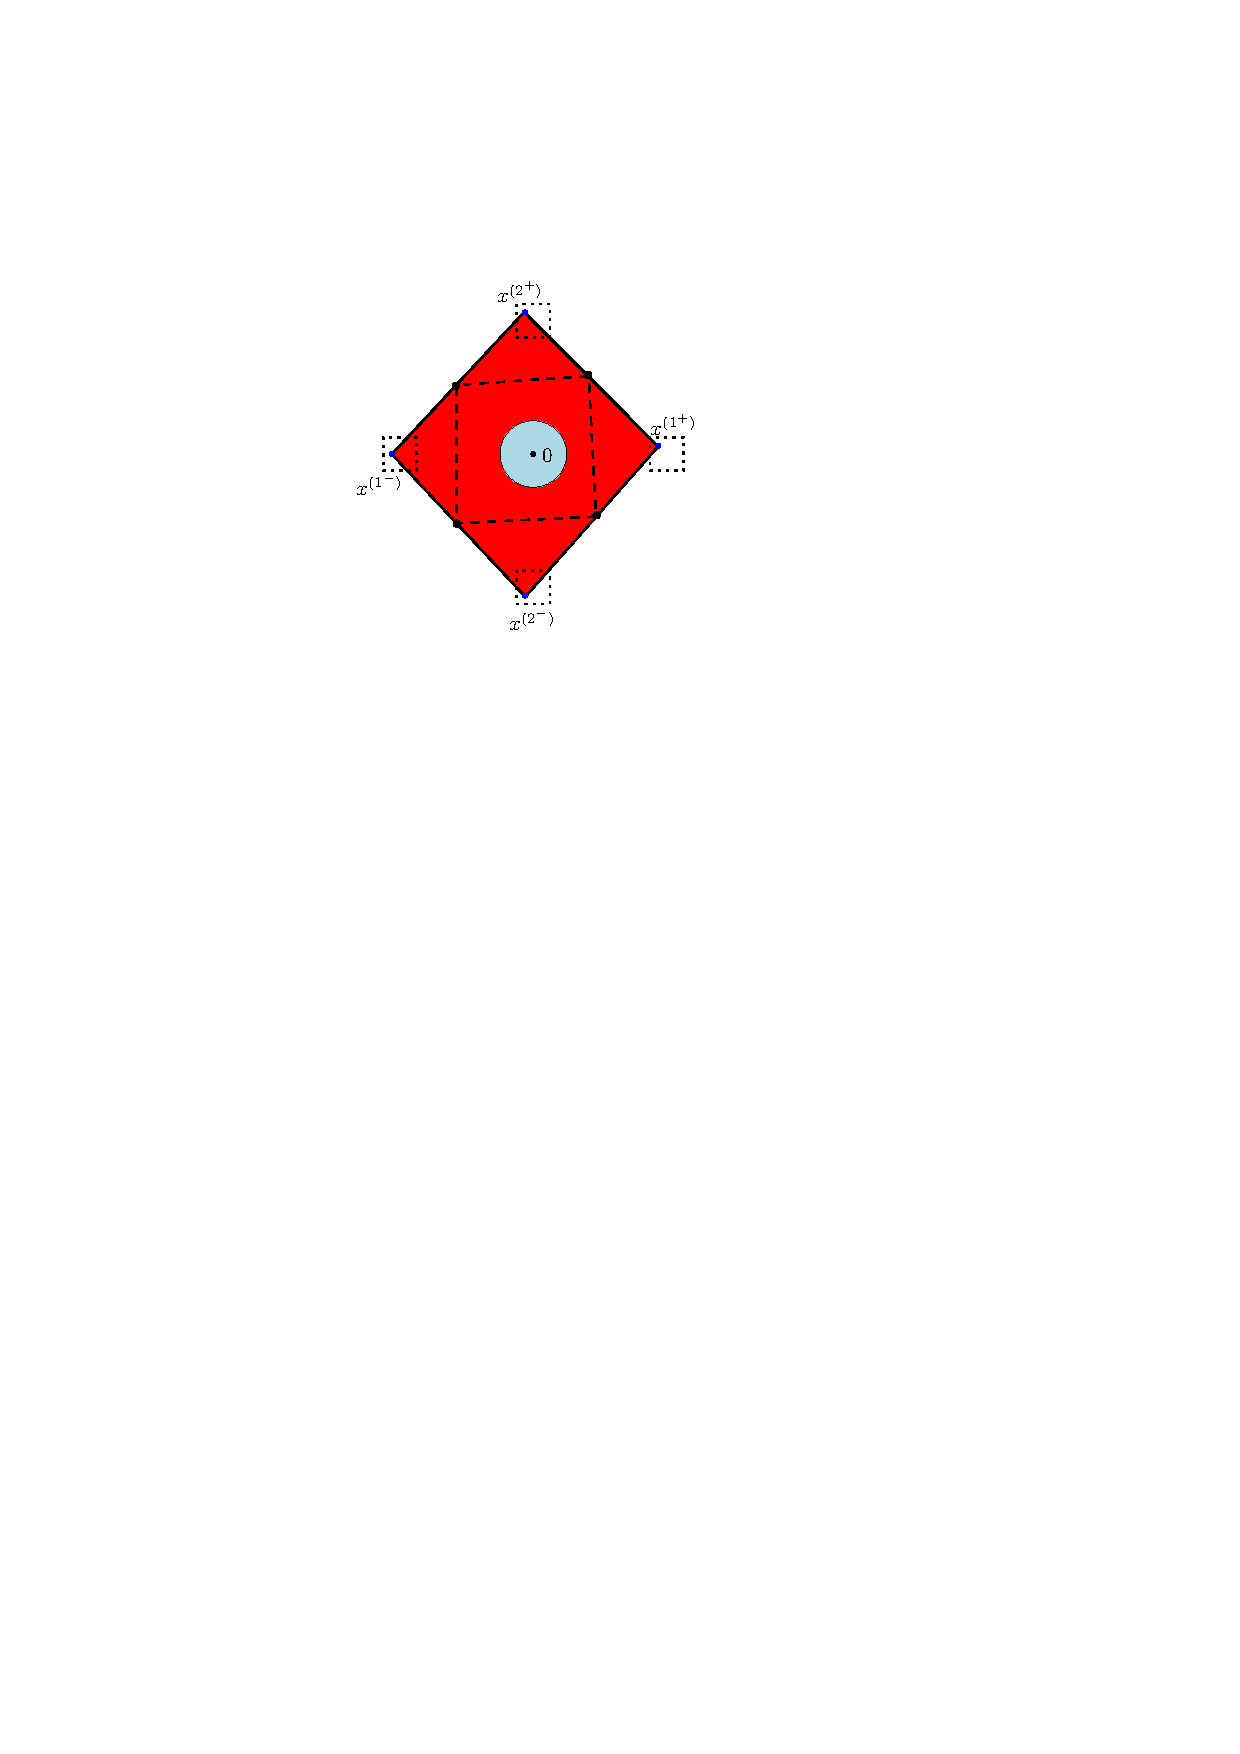
\includegraphics[width=0.5\textwidth]{Figures/nearby-points.pdf}
	\label{fig:nearby-points}
	\caption{Illustration of the proof of Lemma~\ref{lemma:dual-polytope-bound}. The polytope~$P$ is in red and the dual~$P^*$ is outlined by a black dashed line. The cubes~$[-\delta, \delta]^d \pm e_i$ containing~$x^{(i^{\pm})}$, which are blue dots, are outlined by a black dotted line.}
\end{figure}

\begin{lemma} \label{lemma:dual-polytope-bound}
	There exists a constant~$\delta'(d) \in (0,1)$ such that the following holds for every selection of~$x^{(i^{\pm})} \in [-\delta', \delta']^d \pm e_i$ for~$i = 1, \ldots, d$.
	The dual of the convex polytope~$P := \conv(x^{(1^+)}, x^{(1^-)}, \ldots, x^{(d^+)}, x^{(d^-)})$ defined by~$P^* := \{ y \in \Rd: x \cdot y \leq 1 \mbox{ for all~$x \in P$}\}$ is bounded by~$P^* \subset B_{2 \sqrt{d}}$. 
\end{lemma}
% CORRECTION 15: Supply a direct quantitative proof of the unchanged polar bound.
\begin{proof}
Take $\delta'=1/(4d)$. If $y\in P^*$, choose $i$ such that $|y_i|=\|y\|_\infty$ and choose the sign agreeing with $y_i$. The corresponding $x^{(i^\pm)}$ gives
\[
 1\geq x^{(i^\pm)}\cdot y
 \geq\|y\|_\infty-\delta'\sum_j|y_j|
 \geq(1-d\delta')\|y\|_\infty.
\]
Hence $\|y\|\leq\sqrt d\|y\|_\infty\leq(4/3)\sqrt d<2\sqrt d$, as required.
\end{proof}


% CORRECTION 15: Prove both Voronoi criteria on the actual, untranslated grid.
\begin{proof}[Proof of Lemma~\ref{lemma:geometric-constraint}]
For (a), suppose $s\in S\cap U$ and $s'\neq s$ has $\|s'-s\|<2r$. In each coordinate choose $x_i\in r\Z$ by rounding $s_i$ towards $s_i'$ (round up if $s_i'\geq s_i$, down otherwise). Then $|x_i-s_i|\leq r$ and $|x_i-s_i'|<2r$. Thus $s\in x+[-r,r]^d$, so this grid point is tested, while both $s,s'$ belong to $x+[-2r,2r]^d$, a contradiction. All other sites are therefore at distance at least $2r$ from $s$. For $\|z-s\|\leq r$ the triangle inequality gives $\|z-s'\|\geq\|s'-s\|-\|z-s\|\geq\|z-s\|$, proving $B_r(s)\subset\mathcal C_s$.

% CORRECTION 15: Prove part (b) directly on the untranslated grid.
For (b), take $\delta=1/10$ and $R=\max(2,\tfrac{11}{10}\sqrt d)$. Let $s\in S\cap U$, put $a=\tfrac35k\sqrt d$, and suppose that $z\in\mathcal C_s$ satisfies $L:=\|z-s\|>a$. Only finitely many points of $k\Zd$ lie in a bounded set, so there is $\eta\in(0,k]$ such that every grid point $y$ with $\|y-s\|<\tfrac{11}{10}k\sqrt d+\eta$ satisfies $\|y-s\|\leq\tfrac{11}{10}k\sqrt d$. Choose $0<e<\min\{\eta,L-a\}$ and the point $p\in[s,z]$ with $\|p-s\|=a+e$. Round $p$ coordinatewise to a grid point $y\in k\Zd$, so that $\|y-p\|\leq\tfrac12k\sqrt d$. Then $\|y-s\|\leq\tfrac{11}{10}k\sqrt d+e$, hence $\|y-s\|\leq\tfrac{11}{10}k\sqrt d\leq Rk$, and the cube of $y$ is tested. It contains $s''\in S$ with $\|s''-y\|\leq\tfrac1{10}k\sqrt d$, and
\[
 \|s''-z\|\leq\|s''-y\|+\|y-p\|+\|p-z\|
 \leq\tfrac1{10}k\sqrt d+\tfrac12k\sqrt d+L-a-e=L-e<\|s-z\|,
\]
contradicting $z\in\mathcal C_s$. Thus every point of $\mathcal C_s$ is within $\tfrac35k\sqrt d$ of $s$, and $\mathcal C_s\subset B_{4k\sqrt d}(s)$. No translation of the grid has been made.
\end{proof}

% CLOSE 8: An explicit occupied-grid configuration disproves the printed radius starting in dimension thirteen.
\paragraph{Failure of the published test radius for $d\ge13$.}
Let $k=1$, $s=(-1/100,1/2,\ldots,1/2)$, $U=B_{1/1000}(s)$, and
\[
 G=\Zd\cap B_2(U),\qquad S=\{s\}\cup G,\qquad q=s+5\sqrt d\,e_1.
\]
The site set is finite, and every tested grid centre is a site, so every printed occupancy cube contains a site for every $\delta>0$. If $g_1\ge1$, then for $d\ge13$,
\[
 \|g-s\|^2\ge(101/100)^2+(d-1)/4
 \ge40201/10000>(2001/1000)^2.
\]
Such a grid point is not tested, so every $g\in G$ has $g_1\le0$. For $g_1\le-1$,
\[
 \|q-g\|^2-\|q-s\|^2
 =\|g-s\|^2-10\sqrt d\,(g_1+1/100)>0.
\]
For $g_1=0$ the same difference is at least
$(d-1)/4+1/10000-\sqrt d/10>0$; use $\sqrt d\le d$ and $d\ge13$ for the last inequality. Thus $q\in\mathcal C_s$, but $\|q-s\|=5\sqrt d>4\sqrt d$. This is a counterexample under the lemma's exact locally finite site-set hypothesis, so the published radius $2k$ cannot be kept when $d\ge13$.


It remains to show that the conditions of Lemma~\ref{lemma:geometric-constraint} are satisfied with probability one  as~$m \to \infty$
for particular choices of the grid. 



% CORRECTION 16: Use local Poisson estimates, bounded overlap, and a proof for cells meeting U.
\begin{proof}[Proof of Proposition~\ref{prop:min-max-edge-length}]
Fix bounded open sets $U\Subset W_0\Subset W_1\Subset W$, where $\Subset$ means compact containment. All constants below may depend on these sets, the dimension, and the mass exponents. The point processes are indexed by positive integers $m$; no independence between different $m$ is needed. A Poisson process is locally finite almost surely, since its counts on bounded sets of finite intensity are Poisson; use a countable exhaustion by compact sets. The upper mass bound implies that $\mu$ has no atoms in $W$, so the local point process is simple almost surely.

Put $k=m^{-1/(2\beta^+)}$ and $r=m^{-8/\beta^-}$, and let $\delta$ and $R$ be the constants of Lemma~\ref{lemma:geometric-constraint}(b). For all large $m$, every cube used below is contained in $W_1$. Each cube $y+[-\delta k,\delta k]^d$ with $y\in k\Z^d\cap B_{(R+\sqrt d)k}(W_0)$ contains a ball of radius $\delta k$, centred in $W$. Its intensity is at least $m(\delta k)^{\beta^+}=c m^{1/2}$. There are at most $Ck^{-d}$ such grid points. Since the probability of no points in a Poisson variable of mean $\lambda$ is $e^{-\lambda}$, the probability that any of these cubes is empty is at most
\[
 Ck^{-d}e^{-cm^{1/2}},
\]
a summable sequence. Lemma~\ref{lemma:geometric-constraint}(b) therefore bounds every cell whose site belongs to $W_0$ by $B_{4k\sqrt d}(s)$, eventually almost surely.

For the inner bound, consider $Q_x=x+[-2r,2r]^d$ for $x\in r\Z^d$ with $(x+[-r,r]^d)\cap W_0\neq\emptyset$. The upper mass bound gives $\mu(Q_x)\leq C r^{\beta^-}$. These cubes have overlap at most $5^d$, and all lie in the fixed bounded set $W_1$, so $\sum_x\mu(Q_x)\leq5^d\mu(W_1)<\infty$. If $N$ is Poisson of mean $\lambda$, then $\P[N\geq2]\leq\mathbb E[N(N-1)]/2=\lambda^2/2$. A union bound gives
\[
 \P[\exists x:\,|\Lambda_m\cap Q_x|\geq2]
 \leq\tfrac12 m^2\sum_x\mu(Q_x)^2
 \leq C m^2r^{\beta^-}=C m^{-6}.
\]
This is summable too. Borel--Cantelli and Lemma~\ref{lemma:geometric-constraint}(a) give the inner ball for every site in $W_0$.

It remains to include cells meeting $U$ whose sites were not initially known to lie in $W_0$. If $q\in\mathcal C_s\cap U$, round $q$ to a $k$-grid point and use the occupied cube there to find a site $s'$ at distance at most $(1/2+\delta)k\sqrt d$ from $q$. Since $q\in\mathcal C_s$, the same bound holds for $\|s-q\|$. Thus $s\in W_0$ for all large $m$. Finally $4k\sqrt d\leq m^{-1/(3\beta^+)}$ for all large $m$, proving the exact displayed radii.

Apply the same argument to a fixed collar of $\overline U$ compactly contained in $W$ and keep the cells meeting that collar. They are bounded polytopes, and only finitely many occur locally: a locally finite site set has only finitely many sites at bounded distance from a fixed compact set. A bounded Voronoi cell is defined by finitely many of the halfspaces~\eqref{eq:half-space-definition-of-cells}, since sufficiently distant sites cannot cut a fixed ball containing it. These cells give the required local tiling. Its mesh is at most $2m^{-1/(3\beta^+)}$, and the nearest-vertex distance is at most the mesh. Each cell volume is at least $\vol_d(B_1)m^{-8d/\beta^-}$, so the logarithm of the reciprocal minimum volume is $O(\log m)=o(\eps_m^{-1})$. Theorems A and B apply.
\end{proof}








\section{Counterexample for simple random walk} \label{sec:counter-example}
It is straightforward to construct, in all dimensions, sphere packings of \emph{unbounded} degree upon which simple random walk with unit conductance does not converge to Brownian motion modulo time change, see, for example,~\cite[Example 4.8]{NachmiasStFlour}. 
In this section we give a \emph{bounded} degree example in dimensions at least three. This is similar to the potential examples discussed in~\cite[Section 1.5]{GMSInvariance}.
We are not sure whether such a counterexample exists in two dimensions.


\begin{figure}
	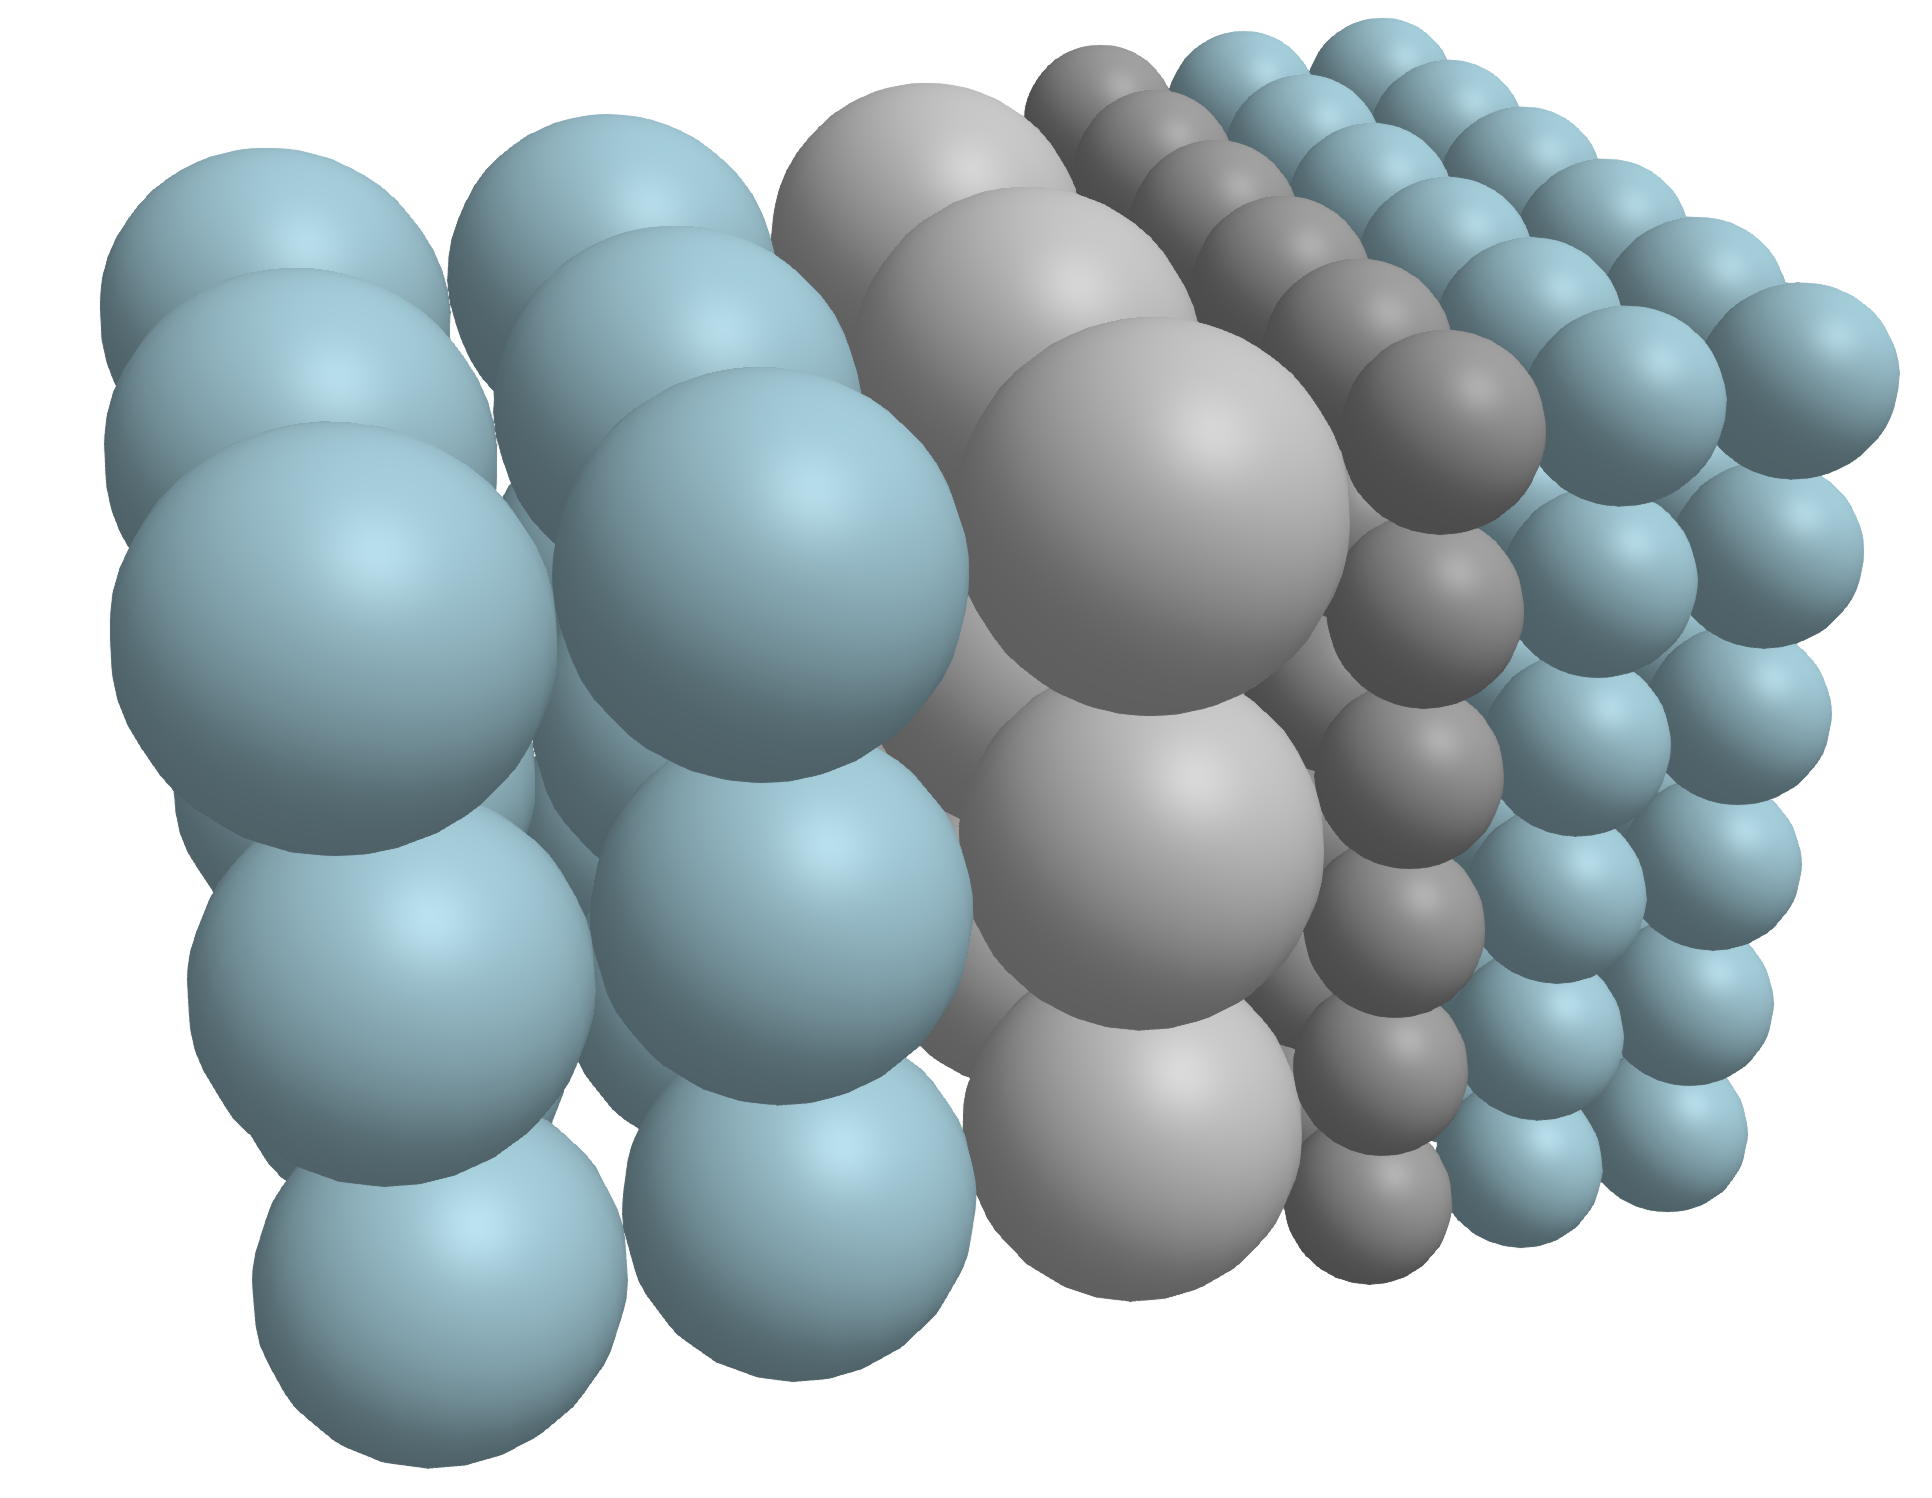
\includegraphics[width=0.45\textwidth]{Figures/sphere-packing3D-angle.png}
	\quad 
	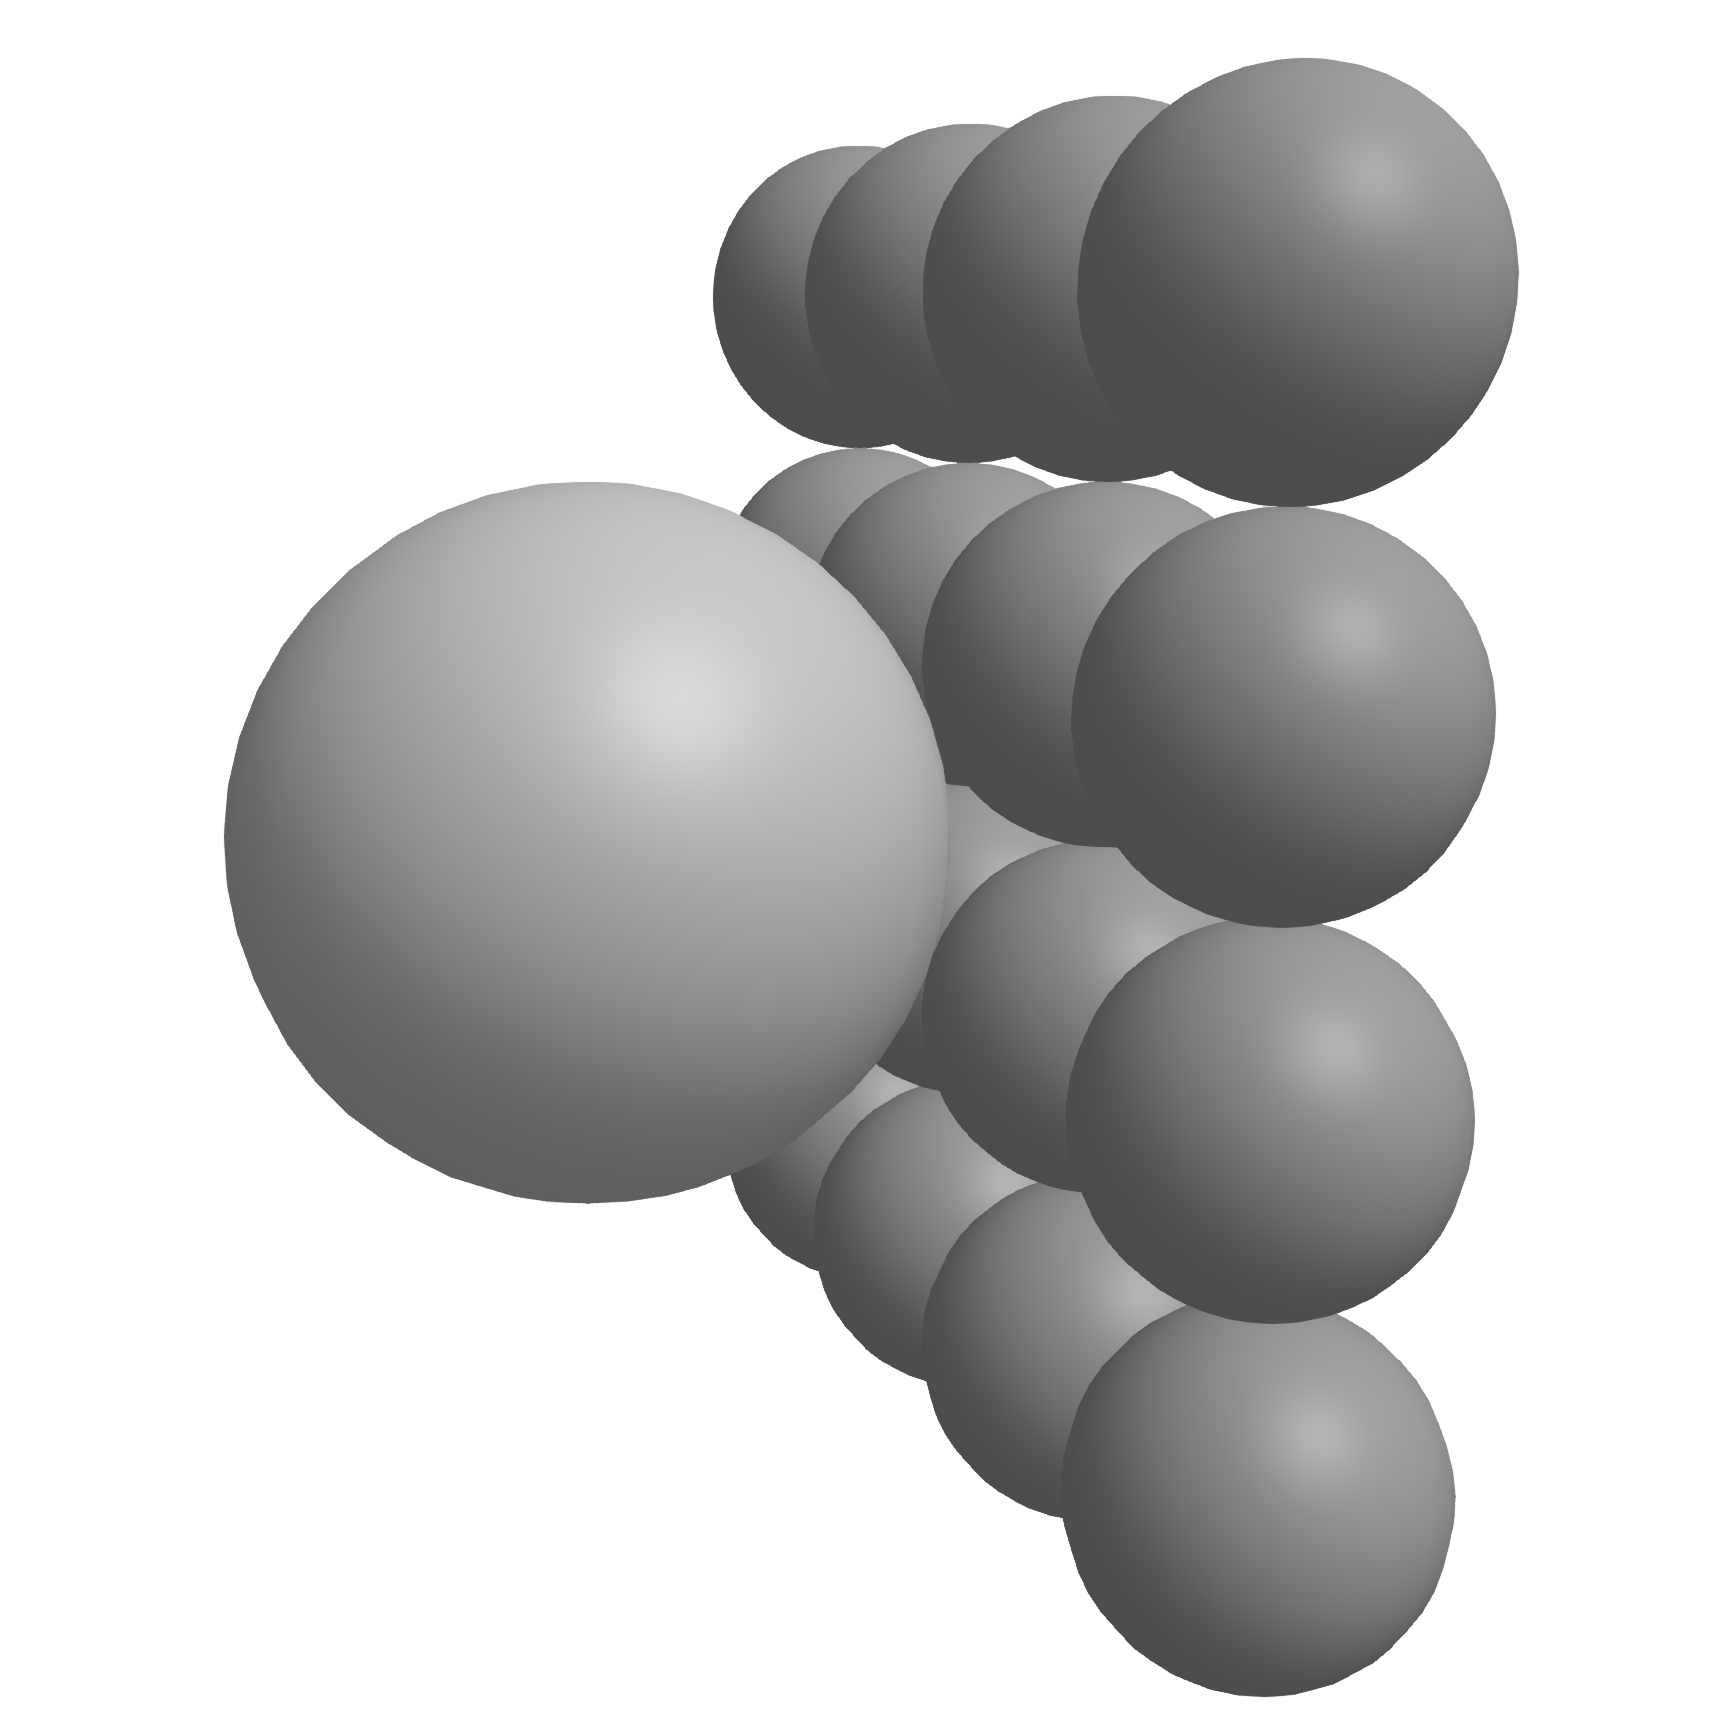
\includegraphics[width=0.35\textwidth]{Figures/spherepack-example3D.png}
	\caption{On the left, part of the sphere packing given in Theorem~\ref{theorem:counter-example} for~$d=3$. 
		On the right, a big middle sphere and some nearby middle small spheres.
		Big  (resp.\ small) middles spheres are in light (resp.\ dark) gray and the other spheres are in light blue.}
	\label{fig:counter-example}
\end{figure}



\begin{theorem} \label{theorem:counter-example}
	For all~$d \geq 3$, there exists a sphere packing of~$\R^d$ upon which simple random 
	walk with unit conductance does not converge to Brownian motion modulo time parametrization in the scaling limit. Moreover, the spheres all have radii either $1$ or $1/2$ and are tangent to a bounded number of other spheres.
\end{theorem}

The sphere packing we construct will force the random walk to lack negation symmetry at large scales, precluding it from converging to Brownian motion.



\begin{figure}
	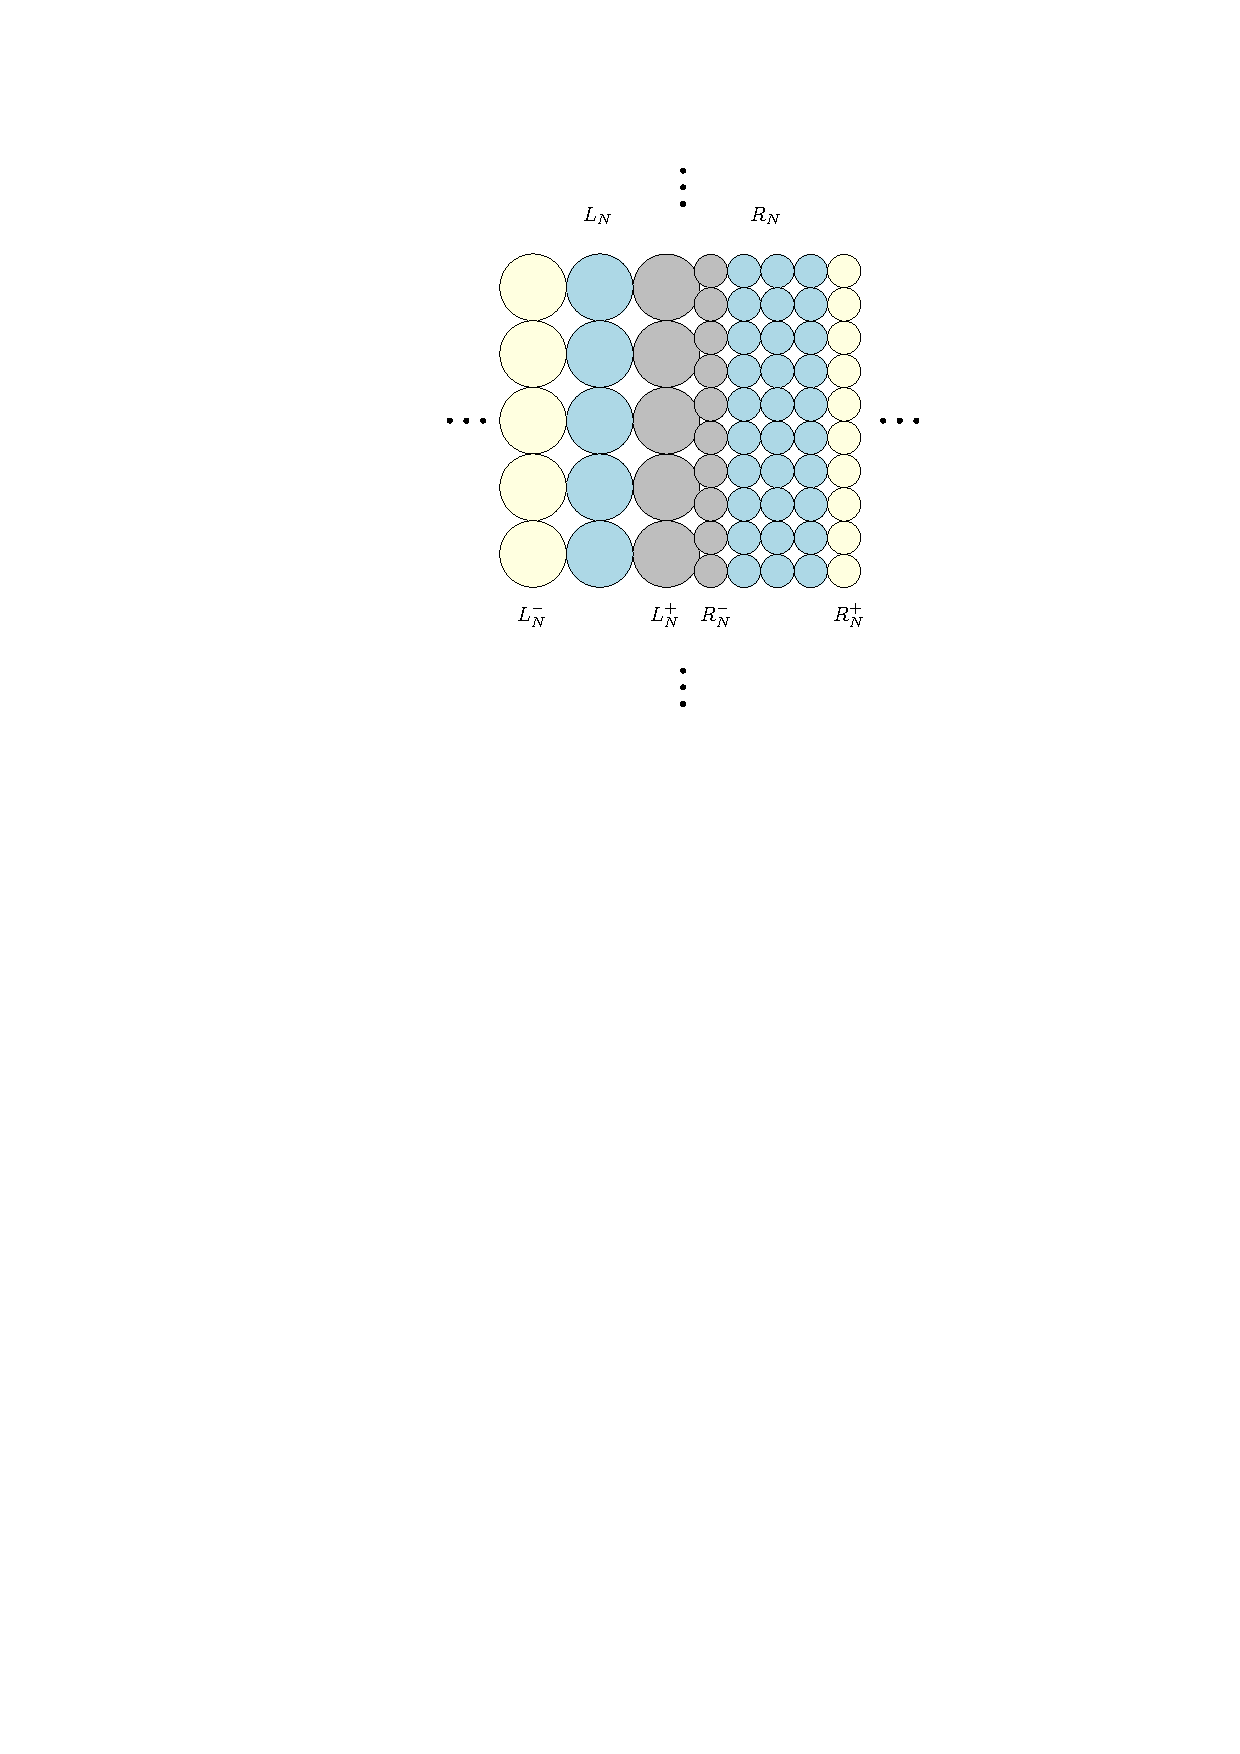
\includegraphics[width=0.5\textwidth]{Figures/slice-of-sphere-packing-labels.pdf}
	\caption{A top-down view of the sphere packing given in Theorem~\ref{theorem:counter-example} for~$d=3$.
		The spheres in~$L_N, R_N$ (defined in~\eqref{eq:def-of-ln}) are in light blue, the spheres in~$L_N^{-}, R_N^{+}$ are in light yellow, 
		the spheres in~$L_N^{+}, R_N^{-}$ are in gray (defined in~\eqref{eq:def-of-lnp}).  Here~$N=2$. Note that the small middle spheres are slightly above small big spheres so they are not overlapping.}
	\label{fig:counter-example-topdown}
\end{figure}



% CORRECTION 17: Keep Theorem 6.1 and repair the construction and the non-convergence proof.
\begin{proof}[Proof of Theorem~\ref{theorem:counter-example}]
Put $a=\sqrt7/2$. Place big spheres of radius $1$ at $2x$, $x\in\Z^d$, $x_1\leq0$. Place small spheres of radius $1/2$ at
\[
 (a,1/2,1/2,0,\ldots,0)+y,\qquad y\in\Z^d,\quad y_1\geq0,
 \quad y_j\in2\Z\ (j\geq4).
\]
For $d=3$ this is the published construction. Distinct big centres are at distance at least $2$, and distinct small centres at distance at least $1$. Between a big and a small centre the smallest possible squared distance is $7/4+1/4+1/4=9/4$. Equality holds exactly for a big middle sphere and the four small middle spheres displaced by $(a,\pm1/2,\pm1/2,0,\ldots,0)$. Thus all interiors are disjoint, each small middle sphere has exactly one big neighbour, and there are no other cross-size contacts. Same-size contacts are coordinate neighbours: in all $d$ directions for big spheres, and in the first three directions for small spheres. Degrees are at most $2d+3$. The graph is connected, since each small layer is connected to a big layer through its middle spheres, and the big half-lattice is connected. For $d\geq4$ the small spheres are not covered in the sense of Section~\ref{subsec:natural-examples}; the theorem does not require that property.

In dimension three this example also has the orthogonal tiling structure mentioned in the introduction. Here is an explicit check, since bounded circumscribed cells alone would not suffice. Away from the interface the tangent-halfspace cells are cubes. For a big middle centre $(0,2i,2j)$ its cell is
\[
 -1\leq x_1\leq\frac{3/2-|x_2-2i|/2-|x_3-2j|/2}{a},\quad
 |x_2-2i|\leq1,\quad |x_3-2j|\leq1.
\]
For each $\sigma,\tau\in\{-1,1\}$, the adjacent small middle centre $(a,2i+\sigma/2,2j+\tau/2)$ has cell
\[
 0\leq u:=\sigma(x_2-2i)\leq1,\quad
 0\leq v:=\tau(x_3-2j)\leq1,\quad
 \frac{3/2-u/2-v/2}{a}\leq x_1\leq a+1/2.
\]
These inequalities follow directly from the tangent planes. The four small cells and the big cell partition the interface slab over each square $[2i-1,2i+1]\times[2j-1,2j+1]$. They join the ordinary cubes at $x_1=-1$ and $x_1=a+1/2$. Their interiors are disjoint, all positive-area contacts are the tangencies already listed, and each centre lies strictly inside its cell. Thus they form a locally finite orthogonal tiling with uniformly bounded cells in dimension three.

For the notation in Figure~\ref{fig:counter-example-topdown}, identify the packing $\mathcal S$ with its centres and, for $N\geq2$, set
\begin{equation}\label{eq:def-of-ln}
 L_N=\{x\in\mathcal S:-2N<x_1<0\},\qquad
 R_N=\{x\in\mathcal S:a<x_1<2N+a\}.
\end{equation}
Their boundary layers are
\begin{equation}\label{eq:def-of-lnp}
 \begin{aligned}
 L_N^-&=\{x\in\mathcal S:x_1=-2N\},&L_N^+&=\{x\in\mathcal S:x_1=0\},\\
 R_N^-&=\{x\in\mathcal S:x_1=a\},&R_N^+&=\{x\in\mathcal S:x_1=2N+a\}.
 \end{aligned}
\end{equation}
Define a function on the centres by $\psi(2x)=4x_1$ at big centres and $\psi((a,1/2,1/2,0,\ldots,0)+y)=y_1+1$ at small centres. It is harmonic for simple random walk. Away from the middle, the first-coordinate increments cancel in pairs and all transverse increments vanish. At a big middle centre the one left increment is $-4$ and the four right increments are $1$. At a small middle centre the increment to its big neighbour is $-1$ and the right increment is $1$; all other increments are zero.

Start the walk at the origin, let $T_n$ be its first exit from the ball of radius $n$, and scale positions by $1/n$. There are finitely many vertices in the ball; connectedness and the finite-path argument for a finite Markov chain show that $T_n<\infty$ almost surely. Jumps have length at most $2$, so the stopped martingale $\psi(X_{t\wedge T_n})$ is bounded for each $n$. Optional stopping (first at $T_n\wedge k$, then bounded convergence) gives $\mathbb E\psi(X_{T_n})=0$.
Put $g(z)=z_1+\min(z_1,0)$. At big centres $\psi(x)/n=g(x/n)$; at small centres their difference is $(1-a)/n$. Hence
\[
 \mathbb E g(X_{T_n}/n)\longrightarrow0.
\]
Brownian motion from zero exits the unit ball with a rotation-invariant distribution on the sphere, so its exit point $Z$ satisfies
$\mathbb E g(Z)=\mathbb E\min(Z_1,0)<0$.
On the ball of radius $3$, $g$ is bounded and Lipschitz; extend its restriction there to a bounded continuous function on $\Rd$. The endpoint map is continuous for~\eqref{eq:cmp-topology}, since every increasing homeomorphism matches endpoints. Convergence of the stopped curve laws would therefore imply convergence of these exit expectations, a contradiction. This proves the theorem with its published statement unchanged.
\end{proof}





{
  \bibliographystyle{plainnat}
  \bibliography{refs}
}




\end{document}
